\documentclass[11pt,singlecolumn, openany, citestyle=authoryear]{elegantbook}

\title{Theory of Probability}
\subtitle{Elegant\LaTeX{} 经典之作}

\author{Jingru Luo}
\institute{New York University Shanghai}
\date{\today}
%\version{4.3}
% \bioinfo{}{}

\extrainfo{春风十里扬州路,卷上珠帘总不如。}

\setcounter{tocdepth}{3}

\logo{logo-blue.png}
\cover{C:/Users/LJR/Desktop/Maths/elegant_math/TheoryOfProbability/figure/white2_2.jpg}
\definecolor{customcolor}{RGB}{32,178,170}
\colorlet{coverlinecolor}{customcolor}
\let\proof\relax
\let\endproof\relax
\usepackage{amsthm}
\usepackage{amsmath}
\usepackage{CJKutf8}
\usepackage{dsfont}
\usepackage{extarrows}
\usepackage{tzplot}
\allowdisplaybreaks[4]
\addbibresource{reference.bib}

\begin{document}
\begin{CJK}{UTF8}{gbsn}
    \maketitle
    \frontmatter
    
    
    \tableofcontents
    
    \mainmatter
    % \chapter*{Preface}
    % \markboth{Introduction}{Introduction}
    % The content of introduction

    \chapter{Basic knowledge}
    \section{Calaulation of sets}\label{sec:CalaulationOfSets}
    \subsection{Intersecton and union}
    Let $\Omega$ be the universe.
    \begin{definition}
        If a set contains all elements of $A,B,\cdots$, it is called the 
        \textbf{union} of $A,B,\cdots$, denoted as 
        $A\cup B \cup \cdots.$
    \end{definition}
    The operation of union is commutative and associative.
    
    \begin{definition}
        Let $A,B,\cdots$ be a set sequence. 
        The set, which consists of elements common to $A,B,\cdots$
        is called the \textbf{intersection} of $A,B\cdots$, denoted as 
        $A \cap B \cdots$(or $AB\cdots$).
    \end{definition}
    
    \begin{definition}
        The set which consists of elements in $\Omega$ but not in $A$, is called
        the \textbf{complement} of $A$, denoted as $A^c$. 
    \end{definition}
    
    For every element in $\Omega$, either it belongs to $A$ or it belongs to 
    $A^c$, i.e. $x \notin A \iff x \in A^c$. Of course, $(A^c)^c = A$.
    
    One can verify that 
    $$
    (A \cup B)^c = A^c \cap B^c, \quad (A \cap B)^c = A^c \cup B^c. 
    $$
    Similarly,
    $$
    \big(\bigcup A_n\big)^c =  \bigcap A_n^c, \quad \big(\bigcap A^n\big)^c = \bigcup A_n^c. 
    $$
    
    In fact, suppose that $x \in \bigcup A_n$, then $x \in A_n$ for some $n$. 
    $x \in \big(\bigcup A_n\big)^c$ implies that for all $n$, $x \notin A_n$, i.e., 
    $x\in A_n^c$. Thus $x \in \bigcap A_n^c$. Hence $\bigcup A_n$ is the complement of
    $\bigcap A_n^c$. One can obtain the second equality by substituting $A_n^c$ with $A_n$.
    
    \begin{figure}[h]
        \centering
        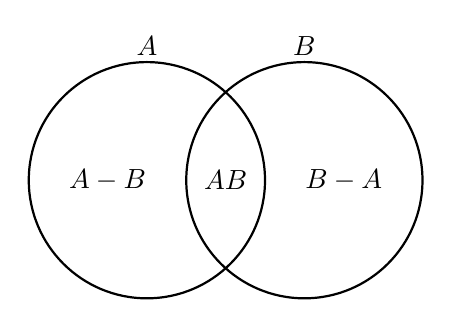
\begin{tikzpicture}
            \draw[thick] (0,0) circle[radius=1.5];
            \draw[thick] (2,0) circle[radius=1.5];
            \node (A) at (0,1.7) {$A$};
            \node (B) at (2,1.7) {$B$};
            \node (C) at (-0.5,0) {$A-B$};
            \node (D) at (1,0) {$AB$};
            \node (E) at (2.5,0) {$B-A$};
        \end{tikzpicture}
    \end{figure}
    
    \begin{definition}
        The set consists of elements that belong to $A$ but not belong to $B$ is 
        denoted as $A-B$. 
    \end{definition}
    One can see that 
    \begin{equation}
        A-B = A-AB = AB^c = B^c-A^c,
    \end{equation}
    $$
    B-A = B-AB = BA^c = A^c-B^c,
    $$
    $$
    A\cup B = (A-B) + (B-A) + AB.
    $$
    Note that the three sets in the right hand side of the last equality are disjoint.
    
    \begin{theorem}
        Let $A,B$ and $C$ be three sets. Then one has the commutative law
    \begin{equation}
    A \cup B = B \cup A, \quad A \cap B = B \cap A; 
    \end{equation}
    the associative law 
    \begin{equation}
        \begin{gathered}
            A \cup (B \cup C) = (A \cup B)\cup C,\\
            A \cap (B \cap C) = (A \cap B)\cap C;
        \end{gathered}
    \end{equation}
    and the distributive law 
        \begin{equation}
            \begin{gathered}
            (A \cup B)\cap C = (A \cap C) \cup (B \cap C),\\
            (A \cap B)\cup C = (A \cup C) \cap (B \cup C).
            \end{gathered}
        \end{equation}
    \end{theorem}
    Similarly, for set sequence, one has
    $$
    \bigcap_i\big(\bigcup_j A_j^{(i)}\big) = 
    \bigcup \big(A_{j_1}^{(1)}\cap A_{j_2}^{(2)}\cap A_{j_3}^{(3)}\cap \cdots\big),
    $$
    $$
    \bigcup_i\big(\bigcap_j A_j^{(i)}\big) = 
    \bigcap \big(A_{j_1}^{(1)}\cup A_{j_2}^{(2)}\cup A_{j_3}^{(3)}\cup \cdots\big),
    $$
    where $j_1,j_2,\cdots$ is a permutation of $1,2,\cdots$.
    
    \begin{theorem}One can use intersection and union to obtain the product of sets, i.e., 
        \begin{equation}
        \bigcap_{n \geq 1}A_n = A_1 - \bigcup_{n \geq 2}\big(A_1-A_n\big).
        \end{equation}
    \end{theorem}
    
    \begin{exercise}
    \begin{enumerate}
        \item Let $A,B$ be two subsets of the whole set $X$. If for any $E \subset X$, one 
        has $E\cap A = E \cup B$, prove that $A=X, B = \varnothing$.
        \item Let $A,B$ be two sets. Prove that 
        $A=B \iff \text{ there is set } C$ such that
        $$
        A \cap C = B \cap C, \quad 
        A \cup C = B \cup C.
        $$
    \end{enumerate}
    \end{exercise}
    \begin{proof}
        \begin{enumerate}
            \item Take $E = X$, we get $A=X$. Take $E=A^c$, we get $B = \varnothing$.
            \item 
            $\Longrightarrow$. Take $C=A$.
            
            $\Longleftarrow$. From 
            $$
            A = A \cap(C \cup C^c) = (A\cap C) \cup (A\cap C^c),
            $$
            we know $A \cup C=(A \cap C^c) \cup C$. Similarly, $B \cup C=(B \cap C^c) \cup C$.
            Note that $C\cap (A \cap C^c) = \varnothing = C \cap(B\cap C^c)$, hence 
            $A \cap C^c = B \cap C^c$, implying 
            $$
            A = (A \cap C)\cup (A \cap C^c) = (B \cap C) \cup (B \cap C^c) = B.
            $$
        \end{enumerate}
    \end{proof}
    
    \subsection{Limit of Set Sequences}
    \begin{definition}
        For a set sequence $\{A_n\}$, let 
        $$
        B_j = \bigcup_{k=j}^\infty A_k (j=1,2,\cdots), \quad 
        C_j = \bigcap_{k=j}^\infty A_k (j=1,2,\cdots),
        $$
        then $B_j \supset B_{j+1}, C_j \subset C_{j+1}, (j=1,2,\cdots)$. We
        define its lime superior $\varlimsup A_n$ and its lime inferior
        $\varliminf A_n$ as 
        \begin{equation}
            \begin{gathered}
            \varlimsup A_n = 
            \lim_{k \to \infty} B_k = \bigcap_{j=1}^\infty B_j =
            \bigcap_{n\geq1} \bigg(\bigcup_{i \geq n} A_i\bigg),\\
            \varliminf A_n = 
            \lim_{k \to \infty} C_k = \bigcup_{j=1}^\infty C_j=
            \bigcup_{n\geq1} \bigg(\bigcap_{i \geq n} A_i\bigg).
            \end{gathered}
        \end{equation}
        When $\varlimsup A_n = \varliminf A_n$, this result is defined as $\lim A_n$.
    \end{definition}
    In convention, one usually uses ``$A_n$ occurs infinitely often'' to read $\varlimsup A_n$
    and ``$A_n$ occurs almost always'' to read $\varliminf A_n$.
    Condider the following statements:
    
    \noindent
    \begin{align*}
    x \in \ \text{infinitely} \ A_n\text{'s} & \iff \forall p \in \mathbb{N}, 
    \exists n \geq p, \ \text{such that}\ x \in A_n\\
    &\iff \forall p \in \mathbb{N}, x \in \bigcup_{n \geq p}A_n \\
    &\iff x \in \bigcap_{p \in \mathbb{N}} \left(\bigcup_{n \geq p}A_n\right)
    \end{align*}
    and
    \begin{align*}
    x \ \text{is in all but a finite number of the}\ A_n \text{'s} & \iff 
    \exists m_x \in \mathbb{N}, \forall n > m_x, x \in A_n\\
    & \iff x\in \bigcup_{m_x \geqslant 1}\left(\bigcap_{n = m_x+1}^{\infty}A_n\right).
    \end{align*}
    
    One can see that $\varlimsup, \varliminf$ have nothing 
    to do with the arrangement of $A_n$. Actually, $\varlimsup A_n$ is the collection of elements
    that are common to \textbf{infinitely} $A_n$ and $\varliminf A_n$ is the collection of elements
    that are common to a `deleted' $A_n$(i.e. \textbf{finite} $A_k$'s are deleted from 
    the original $\{A_n\}$). Hence, we have $\liminf {A_n} \subset 
    \limsup {A_n}$.
    
    When $\{A_n\}$ is increasing, i.e.,
    $A_1 \subset A_2 \subset \cdots \subset A_n \subset \cdots$,
    \begin{equation}
        \lim A_n = \bigcup_{n \geq 1}A_n.
    \end{equation}
    When $\{A_n\}$ is decreasing, i.e.,
    $A_1 \supset A_2 \supset \cdots \supset A_n \supset \cdots$,
    \begin{equation}
        \lim A_n = \bigcap_{n \geq 1}A_n.
    \end{equation}
    Generally, we have
    \begin{equation}
        \varlimsup A_n = \lim_{n \to \infty}\bigcup_{i \geq n}A_i,
        \quad
        \varliminf A_n = \lim_{n \to \infty}\bigcap_{i \geq n}A_i.
    \end{equation}
    For the complement, we have 
    \begin{equation}
        (\varlimsup A_n)^c= \varliminf A_n^c,
        \quad
        (\varliminf A_n)^c = \varlimsup A_n^c.
    \end{equation}
    
    \begin{example}
        Let $E,F$ be two sets. Consider the set sequence 
        $$
        A_F = 
        \begin{cases}
            E, & k \text{ is odd},\\
            F, & k \text{ is even}
        \end{cases}\quad 
        k = (1,2,\cdots),
        $$
        then we have 
        $$
        \varlimsup_{k \to \infty} A_k = E \bigcup F, \quad 
        \varliminf_{k \to \infty} A_k = E \bigcap F.
        $$
    \end{example}
    
    \begin{example}
        Let $\{f_n(x)\}$ and $f(x)$ be real-valued functions defined on $\mathbb{R}$. Then $D$, 
        the set of points where $f_n(x)$ dose not converge to $f(x)$ can be described as 
        $$
        D = \bigcup_{k=1}^\infty \bigcap_{N=1}^\infty \bigcup_{n=N}^\infty 
        \{x: |f_n(x)-f(x)|\geqslant \frac{1}{k}\}.
        $$  
    
        Indeed, if $f_n(x)$ does not converge to $f(x)$ on $x_0$, for a fixed $\varepsilon_0>0$,
        for any natural number $k$, there is $n \geqslant k$ such that
        $$
        |f_n(x)-f(x)|\geqslant \varepsilon_0,
        $$
        i.e., $x_n$ is in infinitely many $E_n$'s, where
        $$
        E_n(\varepsilon_0):=\{x:|f_n(x)-f(x)|\geqslant \varepsilon_0\},
        $$
        namely, $x_n$ is in the lime superior of $\{E_n(\varepsilon_0)\}$.
        Moreover, taking union of $\varepsilon$, the discontinuous points are given
        by the union of these lime superiors. Finally, we use a decreasing sequence 
        $\{\varepsilon_k = 1/k\}$ to supersede $\varepsilon$ and reach our desired $D$.
    \end{example}
    
    \begin{example}
        Let $\{f_n(x)\}$ and $f(x)$ be real-valued functions defined on $\mathbb{R}$ with 
        $$
        \lim_{n \to \infty}f_n(x) = f(x),\quad x \in \mathbb{R}.
        $$
        Then for $t \in \mathbb{R}$, 
    \begin{align*}
        \{x \in \mathbb{R}& : f(x)\leqslant t\}\\
        =& \bigcap_{k=1}^\infty \bigcup_{m=1}^\infty \bigcap_{n=m}^\infty
        \{x\in \mathbb{R}:f_n(x)<t + \frac{1}{k}\}.
    \end{align*}
    
    \end{example}
    
    \subsection{Direct product of sets}
    \begin{definition}
        Let $X,Y$ be two sets. The collection of all ordered ``element pair'' $(x,y)$ (where $x\in X,y \in Y$)
        is called the \textbf{direct product} of $X$ and $Y$, denoted by $X \times Y$, i.e.,
        $$
        X \times Y = \{(x,y):x \in X,y \in Y\},
        $$
        where $(x,y) = (x',y')$ refers to $x=x',y=y'$. $X \times X$ is also denoted by 
        $X^2$.
    \end{definition}

    \section{Mappings and cardinality}
    \begin{definition}
        Let $X,Y$ be two non-empty sets. If for every $x \in X$, there is a unique $y \in Y$
        corresponding to it, we call this corresponding relation a \textbf{mapping}.
        If we use $f$ to denote this relationship, we write 
        $$
        f:X \to Y,
        $$ 
        and $f$ is called a mapping from $X$ to $Y$. Now the unique $y \in Y$ corresponding to 
        a certain $x \in X$ is called the \textbf{image} of $x$ under $f$ whereas $x$ is called
        a \textbf{pre-image} of $y$, denoted by $f(x)=y$. 
        If for any $y \in Y$, there is $x \in X$ such that $f(x)=y$, $f$ is called a \textbf{surjection}
        of $f$ from $X$ to $Y$.
    \end{definition}
    
    For $f:X \to Y$ and $A \subset X$, we write 
    $$
    f(A)=\{y \in Y:x \in A,y=f(x)\}
    $$
    with stipulation $f(\varnothing) = \varnothing$.
    Clearly, 
    \begin{enumerate}[(i)]
        \item $\displaystyle f \left(
        \bigcup_{\alpha \in I}A_\alpha    
        \right)=\bigcup_{\alpha \in I}f(A_\alpha)$;
        \item $\displaystyle f\left(
            \bigcap_{\alpha \in I}A_\alpha    
            \right)\subset \bigcup_{\alpha \in I}f(A_\alpha)$.
    \end{enumerate}
    
    For $f:X \to Y$ and $B \subset Y$, we write 
    $$
    f^{-1}(B) = \{x \in X: f(x) \in B\}.
    $$
    Similarly,
    \begin{enumerate}[(i)]
        \item for $B_1 \subset B_2$, we have $f^{-1}(B_1)\subset f^{-1}(B_2)$;
        \item $\displaystyle 
        f^{-1}\left(
        \bigcup_{\alpha \in I}B_\alpha    
        \right)=\bigcup_{\alpha \in I}f^{-1}(B_\alpha)
        (B_\alpha \subset Y, \alpha \in I)
        $;
        \item $\displaystyle 
        f^{-1}\left(
        \bigcap_{\alpha \in I}B_\alpha    
        \right)=\bigcap_{\alpha \in I}f^{-1}(B_\alpha)
        (B_\alpha \subset Y, \alpha \in I)
        $;
        \item $\displaystyle 
        f^{-1}(B^c) = (f^{-1}(B))^c
        (B \subset Y)
        $.
    \end{enumerate}
    
    \begin{definition}
        Let $f:X \to Y$. If $f$ satisfies that for $x_1,x_2\in X$ and $x_1\neq x_2$,
        $$
        f(x_1)\neq f(x_2),
        $$
        $f$ is called an \textbf{injection} from $X$ to $Y$. If $f$ is both injective and 
        surjective, $f$ is called a \textbf{bijection} from $X$ to $Y$. Take $f$ bijective
        from $X$ to $Y$, then for every $y \in Y$, there is a unique $x \in X$ such that 
        $f(x)=y$, i.e., there is a mapping 
        $$
        g:Y \to X, \quad g(y)=x,
        $$
        where $x$ is determined by $y=f(x)$. $g$ is then called the \textbf{inverse} of 
        $f$, denoted as $f^{-1}$.
    \end{definition}
    
    \begin{definition}
        The \textbf{indicator mapping} of set $A$, denoted as $\mathds{1}_A$, is defined as 
        \begin{equation}
            \mathds{1}_A(x) :=
            \begin{cases}
                1,\ \text{if}\ x \in A \\
                0,\ \text{if}\ x \notin A.
            \end{cases}
        \end{equation}
    \end{definition}
    
    \begin{example}
        Show that
        $$
        \mathds{1}_{\limsup A_n} = \limsup \mathds{1}_{A_n}, \ \text{and} \ 
        \mathds{1}_{\liminf A_n} = \liminf \mathds{1}_{A_n}.
        $$
    \end{example}
    \begin{proof}
        Observe that both mappings $\mathds{1}_{\limsup A_n}$ and $\limsup \mathds{1}_{A_n}$
        only take values in $\{0,1\}$.
    
        For an arbitrary $x \in \Omega$, consider the following statements:
        \begin{align*}
            \mathds{1}_{\limsup A_n} = 1 &\iff x \in \varlimsup A_n\\
            &\iff \forall p \in \mathbb{N}, \exists n \geq p, \ \text{such that}\ 
            x \in A_n \\
            &\iff \forall p \in \mathbb{N}, \exists n \geq p, \ \text{such that}\ 
            \mathds{1}_{A_n}(x) = 1\\
            &\iff \limsup \mathds{1}_{A_n}(x) = 1.
        \end{align*}
    \end{proof}
    
    \begin{definition}
        Let $X$ be a non-empty set. The collection of all subsets of $X$ (including
        $\varnothing$ and $X$) is called the \textbf{power set} of $X$, denoted as 
        $\mathcal{P}(X)$.
    \end{definition}
    For example, there are $2^n$ elements in the power set of an $n$-element set $E$.
    \begin{example}[(Fixed points of monotonous mappings)]
        Let $X$ be a non-empty set. Let $f:\mathcal{P}(X) \to \mathcal{P}(X)$ satisfying 
        $f(A) \subset f(B)$ for any $A\subset B \in \mathcal{P}(X)$, then there is 
        $T \subset \mathcal{P}(X)$ such that $f(T)=T$.
    \end{example}
    \begin{proof}
        Consider sets $S$ and $T$, where
        \begin{align*}
            S &= \{A:A\in\mathcal{P}(X) \text{ and } A \subset f(A)\}, \\
            T &= \bigcup_{A \in S}A (\in \mathcal{P}(X)).
        \end{align*}
        I claim that $f(T)=T$.
        
        Indeed, from $A \in S$ we know that $A \subset f(A)$. Moreover, $A \subset T$, implying 
        that $f(A) \subset f(T)$, hence we deduce $f(A)\subset f(T)$ from $A \in S$, following
        $$
        \bigcup_{A \in S}A \subset f(T), \quad T \subset f(T).
        $$
    
        On the other hand, based on $T \subset f(T)$, we know $f(T) \subset f(f(T))$, implying 
        $f(T) \in S$ thus $f(T) \subset T$. 
    \end{proof}

\chapter{Measure theory and probability spaces}
\section{Algebras and $\sigma$-algebras}
\begin{definition}
    Let $E$ be a set and let $\mathcal{A} $ be a \textbf{set of subsets} of $E$.
    We say that $\mathcal{A}$ is an algebra if for all $B,A \in \mathcal{A}$,
    $$
    \varnothing \in \mathcal{A}, A^c \in \mathcal{A},\ \text{and}\ A\bigcup B \in \mathcal{A}.
    $$
    We say that $\mathcal{A}$ is a $\pi$-system if for all $B,A \in \mathcal{A}$,
    $$
    \varnothing \in \mathcal{A}, \ \text{and} \ A\bigcap B \in \mathcal{A}.
    $$
    We say that $\mathcal{A}$ is a $\lambda$-system if 
    \begin{gather*}
    \varnothing \in \mathcal{A}, \ \text{and} \ B\setminus A \in \mathcal{A}
    \text{ given } A,B \in \mathcal{A}, A \subseteq B, \text{ and }\\
    A \in \mathcal{A} \text{ given } A_n \uparrow A, A_n \in \mathcal{A}.
    \end{gather*}
    We say that $\mathcal{A}$ is a $\sigma$-algebra if for all $A \in \mathcal{A}$,
    and all sequences $\{A_n\}_{n \in \mathbb{N}}$,
    $$
    \varnothing \in \mathcal{A}, A^c \in \mathcal{A}, \ \text{and} \ 
    \bigcup_{n \in \mathbb{N}}A_n \in \mathcal{A}.
    $$
\end{definition}
Immediately, we have the following lemmas:

\begin{lemma}
    Every $\sigma$-algebra is an algebra.
\end{lemma}

\begin{lemma}
    Every algebra is a $\pi$-system.
\end{lemma}

\begin{example}
    $\mathcal{A} = \{\varnothing, E\}$ is a(n) ($\sigma$-)algebra, ususally called the trivial 
    ($\sigma$-)algebra.
\end{example}

\begin{example}
    The power set $\mathcal{P}(E):=\{A:A \subset E\}$ is a(n) ($\sigma$-)algebra.
\end{example}

\begin{lemma}
    The intersection of any collection of ($\sigma$-)algebras is a(n) ($\sigma$-)algebra, i.e.,
    if $\mathcal{A}_1$ and $\mathcal{A}_2$ are both ($\sigma$-)algebras, 
    then their intersection
    $\mathcal{A}_1 \cap \mathcal{A}_2$ is also a(n) ($\sigma$-)algebra. 
\end{lemma}

\begin{definition}\label{def:generated}
    Note that the intersection of any collection of $\sigma$-algebras is a 
    $\sigma$-algebra. Thus for any set of
subsets $\mathcal{C} $ the intersection of all the $\sigma$-algebras 
(there is at least one) containing $\mathcal{C} $ is itself a
$\sigma$-algebra. We call this the $\sigma$-algebra generated by $\mathcal{C}$,
and we denote it by $\sigma(\mathcal{C})$. Similarly, the intersection of all the algebras 
(there is at least one) containing $\mathcal{C} $ is itself an algebra. 
We call this the algebra generated by $\mathcal{C}$,
and we denote it by $a(\mathcal{C})$. To be more precise,
\begin{gather*}
    \sigma(\mathcal{C}) = \bigcap_{\substack{\mathcal{A} \text{ is a $\sigma$-algebra}\\
    \mathcal{C}\subseteq \mathcal{A}}}\mathcal{A};\\
    a(\mathcal{C}) = \bigcap_{\substack{\mathcal{A} \text{ is an algebra}\\
    \mathcal{C}\subseteq \mathcal{A}}}\mathcal{A}.
\end{gather*}
\end{definition}
Based on definition \ref{def:generated}, we know 
\begin{proposition}
    $\sigma(\mathcal{C})$ is the smallest $\sigma$-algebra containing $\mathcal{C}$
    whereas $a(\mathcal{C})$ is the smallest algebra containing $\mathcal{C}$.
\end{proposition}

\begin{proposition}
    Let $\mathcal{C}$ be a set of subsets. Then 
    $$
    a(\mathcal{C})\subseteq \sigma(\mathcal{C}), \quad 
    \sigma(a(\mathcal{C}))= \sigma(\mathcal{C}).
    $$
\end{proposition}
\begin{proof}
    The first assertion is trivial since every $\sigma$-algebra is an algebra.
    For the second one, first note that $\mathcal{C} \subseteq a(\mathcal{C})$ thus
    $\sigma(a(\mathcal{C}))$ is actually a $\sigma$-algebra containing $\mathcal{C}$, implying
    $\sigma(\mathcal{C})\subseteq \sigma(a(\mathcal{C}))$.   
    Conversely, since $a(\mathcal{C})\subseteq \sigma(\mathcal{C})$, we know that 
    $\sigma(\mathcal{C})$ is a $\sigma$-algebra containing $a(\mathcal{C})$. Hence 
    $\sigma(a(\mathcal{C}))\subseteq \sigma(\mathcal{C})$.
\end{proof}

\begin{example}
    For $A \subseteq E$, 
    let $\mathcal{C}=\{\varnothing, A\}$. Then 
    $a(\mathcal{C})=\{\varnothing, A, A^c, E\}$.
\end{example}
\begin{proof}
    We use the shorthand $\mathcal{F}=\{\varnothing, A, A^c, E\}$. It is easy to observe 
    that $\mathcal{F}$ is an algebra containing $\mathcal{C}$.
    Then $a(\mathcal{C}) \subseteq \mathcal{F}$ according to the ``smallest'', implying 
    $a(\mathcal{C})\subseteq \mathcal{F}$.

    On the other hand, for every member in $\mathcal{F}$, they are in $a(\mathcal{C})$,
    implying $\mathcal{F}\subseteq a(\mathcal{C})$.
\end{proof}

\begin{example}
    Let $\pi=\{A_1,A_2,\cdots,A_n\}$ be a partition of $E$, i.e., $A_i \cap A_j = \varnothing$
    and $\displaystyle \bigcup_{i=1}^m A_i=E$. Then 
    \begin{align*}
        a(\pi) &= \{\text{finite disjoint unions of } \{A_i\}_{i=1}^m\}\\
        &= \bigg\{\bigcup_{i \in I}A_i \text{ for some } I 
        \subseteq \{1,2,\cdots,m\}\bigg\}.
    \end{align*}
\end{example}

\begin{example}
    Let $\mathcal{A}$ be an algebra of $\mathbb{R}$ and $X: E \to \mathbb{R}$ be a set function.
    Then $\{X^{-1}(A):A \in \mathcal{A}\}$ is an algebra where $X^{-1}(A):=\{\omega \in E:
    X(\omega) \in A\}$.
\end{example}

\begin{example}\label{eg:eg1}
    Let $\mathcal{E}$, a set of subset of $\mathbb{R}$ 
    be $\mathcal{E}=\{(a,b]:-\infty \leqslant a < b \leqslant +\infty,
    (a,+\infty):a \in \mathbb{R}\}$.
    Then $a(\mathcal{E})=\{I_1\cup I_2\cup \cdots \cup I_n, I_k \in \mathcal{E},
    I_i \cap I_j = \varnothing, 1 \leqslant i,j,k \leqslant n\}$.
\end{example}

\begin{example}[($\pi$-systems generating $\mathcal{B}(\mathbb{R})$)]
    The followings are four methods to generate $\mathcal{B}(\mathbb{R})$:
    \begin{enumerate}
    \item $\mathcal{E}_1:=\{(a,b]:-\infty \leqslant a \leqslant b < +\infty\}$ is a 
    $\pi$-system.
    \item $\mathcal{E}_2:=\{(a,b):-\infty \leqslant a \leqslant b \leqslant +\infty\}$ is a 
    $\pi$-system.
    \item $\mathcal{E}_3:=\{A\subset \mathbb{R}:A \text{ is open}\}$ is a 
    $\pi$-system.
    \item $\mathcal{E}_4:=\{A\subset \mathbb{R}:A \text{ is closed}\}$ is a 
    $\pi$-system.
    \end{enumerate}
\end{example}
\begin{proof}
    Only for 3.
    It suffices to show $\sigma(\mathcal{E}_2)=\sigma(\mathcal{E}_3)$.
    $\sigma(\mathcal{E}_2)\subset \sigma(\mathcal{E}_3)$ is trivial since $\mathcal{E}_2 \subset \mathcal{E}_3$. 
    Conversely, let $A\subseteq \mathbb{R}$ be open, and then 
    $$
    A=\bigcup_{i=1}^\infty (x_i-\varepsilon_i,x_i+\varepsilon_i)
    $$
    implying $\mathcal{E}_3 \subset \sigma(\mathcal{E}_2)$ and thus 
    $\sigma(\mathcal{E}_3)\subset\sigma(\mathcal{E}_2)$ according to the ``smallest''.
\end{proof}

\begin{exercise}
    Let $\mathcal{A}$ be an algebra on $E$. If $A \notin \mathcal{A}$
    and $B \notin \mathcal{A}$, is it the same for $A \cup B$ and $A \cap B$?
\end{exercise}
\begin{proof}[Solution]
    Let $E=\{0,1\}, \mathcal{A}=\{\varnothing, E\}, A=\{1\}, B = \{0\}$.
    Then $A \cap B = \varnothing \in \mathcal{A}$ and $A \cup B = E \in \mathcal{A}$.
\end{proof}

\begin{exercise}
    Provide a counterexample in which $\mathcal{A} \cup \mathcal{B}$ is not an algebra 
    whereas $\mathcal{A}$ and $\mathcal{B}$ are both algebras, seperately. 
\end{exercise}
\begin{proof}[Solution]
    Set $\Omega = \{0,1,2\}, A = \{0\}, B = \{0,1\}$. Then $a(A)=\{\varnothing,\Omega,
    A,A^c\},a(B)=\{\varnothing,\Omega,B,B^c\}$. Note that 
    $a(A)\cup a(B)=\{\varnothing,\{0\}, \{0,1\},\{2\},\{1,2\},\Omega\}$ whereas 
    $\{0,1\}\cap \{1,2\}=\{1\}\notin a(A)\cup a(B)$.
\end{proof}

\begin{exercise}
    Let $E$ be an infinite set (countable or not). Let $\mathcal{A}$ be the set of
    subsets of $E$ that are either finite or with finite complement in $E$. Prove that 
    $\mathcal{A}$ is an algebra but not a $\sigma$-algebra. 
\end{exercise}
\begin{proof}
    Take a subset $A$ of $E$ where $A \in \mathcal{A}$. If $A$ is finite, its complement 
    must also be in $\mathcal{A}$ since $(A^c)^c=A$. If $A^c$ is finite, it is the same.
    This has already implied $\varnothing,E \in \mathcal{A}$.
    
    Now take another $B \subseteq E$ with $B \in \mathcal{A}$. 
    If $A$ and $B$ are both finite, $A \cup B$ is also finite thus in $\mathcal{A}$. We 
    finished the proof. Otherwise, assume $A$ is not finite. Note that 
    $(A \cup B)^c = A^c \cap B^c$ is finite since $A^c$ is finite. Hence $A \cup B$ is indeed
    in $\mathcal{A}$.

    Now assume that $\mathbb{N}\subset E$. Consider the even number set 
    $2\mathbb{N}=\{2n,n\in\mathbb{N}\}$. If $\mathcal{A}$ is a $\sigma$-algebra,
    since each $\{n\}$ is in $\mathcal{A}$, their countable union $2\mathbb{N}$ must also 
    be in $\mathcal{A}$. However, neither $2\mathbb{N}$ nor $E\setminus 2\mathbb{N}$ is finite.
\end{proof}

\begin{exercise}
    Let $\Omega = \mathbb{N}$. For $n \geqslant 0$, let $\mathcal{F}_n=\sigma(\{
        \{0\},\cdots,\{n\}
    \})$, the smallest $\sigma$-algebra containing all of $\{0\},\cdots,\{n\}$.
    Show that $\displaystyle \bigcup_{n \geqslant 0}\mathcal{F}_n$ is not a 
    $\sigma$-algebra.
\end{exercise}
\begin{proof}
    Let us write down several $\mathcal{F}_n$'s.
    \begin{gather*}
        \mathcal{F}_0 = \{\varnothing,\mathbb{N},\{0\},\mathbb{N}\setminus\{0\}\};\\
        \mathcal{F}_1 = \{\varnothing,\mathbb{N},\{0\},\{1\},
        \mathbb{N}\setminus\{0\},\mathbb{N}\setminus\{1\},
        \mathbb{N}\setminus\{0,1\}
        \};\\
        \vdots
    \end{gather*}  
    We can obsrve that for each natural even number $2k$, $\{2k\} \in \displaystyle \bigcup_{n \geqslant 0}\mathcal{F}_n$,
    whereas $2\mathbb{N}$ does not belong to $\displaystyle \bigcup_{n \geqslant 0}\mathcal{F}_n$.
\end{proof}

\section{Measurable spaces}
\begin{definition}
    A pair $(E, \mathcal{E} )$, where $E$ is a set and $\mathcal{E} $ 
    is a $\sigma$-algebra on $E$, is called a measurable space.
Given a measurable space $(E, \mathcal{E} )$ each $A \in \mathcal{E} $ 
is called a measurable set (or an $E$-measurable set). 
\end{definition}
Recall the set $\mathcal{E}$ in Example \ref{eg:eg1}. We have had an understanding of $a(\mathcal{E})$.
Now let's take a look at $\sigma(\mathcal{E})$. First, one can observe that any single
point $\{a\}, a \in \mathbb{R}$ is in $\sigma({\mathcal{E}})$ since $\{a\}=
\displaystyle \bigcup_{n \geq 1}(a-\dfrac{1}{n},a]$. Thus every countable set (for example,
$\mathbb{Q}$ and transcendental numbers) is also in $\sigma(\mathcal{E})$. Moreover, every open interval $(a,b)$ is in 
$\sigma(\mathcal{E})$ since $(a,b)=\displaystyle \bigcup_{n \geqslant 1}(a,b-\dfrac{1}{n})$.
Finally, $[a,b)$ is in $\sigma(\mathcal{E})$ since $[a,b)=
\displaystyle \bigcup_{n \geqslant 1}[a,b-\dfrac{1}{n})$. Thus, $\sigma(\mathcal{E})$ actually
basically contains the ``nice subsets of $\mathbb{R}$'', usually it is called the 
\textbf{Borel set of $\mathbb{R}$}, denoted as $\mathcal{B}(\mathbb{R})$.

We will keep using the notation $\mathcal{E}$ to represent the set mentioned in 
Example \ref{eg:eg1} in this section if not specifically stated.

\begin{definition}
    Let $E$ be a set, and let $\mathcal{A}$ be an algebra on $E$.
A set function is any function $\mu : \mathcal{A} \to [0, \infty]$ with $\mu (\varnothing ) = 0$.
\end{definition}

Let $\mu$ be a set function.
We say that $\mu$ is increasing if, for all $A, B \in \mathcal{A}$ with $A \subseteq B$,
$$
\mu(A) \leq \mu(B).
$$
We say that $\mu$ is additive if, for all disjoint sets $A, B \in \mathcal{A}$,
$$
\mu(A \cup B) = \mu(A) + \mu(B).
$$
We say that $\mu$ is countably additive if, for all sequences of disjoint sets 
$\{A_n\}_{n\in \mathbb{N}} \subseteq \mathcal{A}$, with
$\displaystyle \bigcup_{n \in \mathbb{N}} A_n \in \mathcal{A}$, we have
$$
\mu(\bigcup_{n \in \mathbb{N}} A_n) = \sum_{n \in \mathbb{N}} \mu(A_n).
$$

\begin{definition}
    Let $\mathcal{A}$ be an algebra (of subsets of $E$). A set function $\mu:
    \mathcal{A} \to [0,+\infty)$ is called a \textbf{content} if 
    \begin{enumerate}
        \item $\mu(\varnothing)=0$;
        \item $\mu$ is finitely additive.
    \end{enumerate}
\end{definition}
\begin{lemma}
    Let $\mu:\mathcal{A} \to [0,+\infty)$ be a content. Then for any $A,B \in \mathcal{A}$,
    \begin{enumerate}
        \item $\mu(A \cup B) +\mu(A \cap B) = \mu(A)+\mu(B)$;
        \item If $A \subseteq B$ and $\mu(A)< +\infty$ then 
        $\mu(B \setminus A)=\mu(B)-\mu(A)$;
        \item If $A \subseteq B$, then $\mu(A)\leqslant \mu(B)$.
        \item (Subadditivity) If $A_1,A_2,\cdots,A_n \in \mathcal{A}$, then 
        $$
        \mu(\bigcup_{i=1}^n A_i)\leqslant \sum_{i=1}^n \mu(A_i).
        $$
        \item ($\sigma$-superadditivity) If $\{A_i\}_{i=1}^{+\infty}$ is a sequence of disjoint elements and 
        $\displaystyle \bigcup_{i\geqslant 1}A_i \in \mathcal{A}$, then 
        $$
        \mu(\bigcup_{i \geqslant 1}A_i) \geqslant \sum_{i\geqslant 1}\mu(A_i).
        $$
    \end{enumerate}
\end{lemma}
\begin{proof}
    Only prove 5. By 4, we have for any $N\in\mathbb{N}$
    $$
    \mu\bigg(\bigcup_{i=1}^N A_i\bigg) \leqslant \sum_{i=1}^N \mu(A_i).
    $$
    Thus the superadditivity holds by nature since by 3,
    $$
    \mu\bigg(\bigcup_{i=1}^\infty A_i\bigg) \geqslant \mu\bigg(\bigcup_{i=1}^N A_i\bigg)
    \geqslant \sum_{i=1}^N \mu(A_i).
    $$
\end{proof}
\begin{example}[(Density of $\mathbb{R}$)]
    Let $E = \mathbb{R}$ and $\mathcal{A}=a(\mathcal{E})$. For any $A \in a(\mathcal{E})$,
    define $\displaystyle \mu(A)=\lim_{L \to \infty}\dfrac{|A \cap (0,L)|}{L}$. Then 
    $\mu$ is finitely additive but not countably additive. In fact, note that  
    $$
    1 = \mu(\bigcup_{i\geqslant 0}[i,i+1)) > \sum_{i\geqslant 0}\mu([i,i+1))=0.
    $$
\end{example}

\begin{definition}
    Let $(E, \mathcal{E})$ be a measurable space. 
    A countably additive set function $\mu : E \to [0,\infty]$ is called
    a measure; the triple $(E, \mathcal{E}, \mu)$ is called a measure space.
\end{definition}

\begin{example}\label{eg:egm}
    Let $E = \mathbb{R}$. Define a set function $m:a(\mathcal{E})\to [0,+\infty]$. Let 
    $m((a,b])=b-a, m((a,+\infty))=+\infty$ and extend for every $A \in a(\mathcal{E})$, i.e.,
    $\displaystyle m(A)=\sum_{j=1}^n m(I_j)$ where $\displaystyle A=\bigcup_{j=1}^n I_j$ and 
    $I_j$'s are two by two disjoint. Then $m$ is actually a content.
\end{example}

\begin{lemma}
    The set function $m$ defined in Example \ref{eg:egm} is countably additive, i.e.,
    for $\{A_k\}_{k=1}^\infty \subset a(\mathcal{E})$ such that $A_k$'s are two by two 
    disjoint and $\displaystyle A=\bigcup_{k\geqslant 1}A_k \subset a(\mathcal{E})$, one has 
    $m(A) = \displaystyle \sum_{k\geqslant 1}m(A_k)$.
\end{lemma}
\begin{proof}
    We introduce a new partition of $A$, i.e., set 
    $A = \displaystyle \bigcup_{i=1}^n I_i$, where every $I_i \in \mathcal{E}$ is disjoint 
    with each other. Moreover, let 
    $A_k = \displaystyle \bigcup_{j=1}^{m_k} J_{j,k}$, where where every $J_{j,k} \in \mathcal{E}$
    is disjoint with respect to $j$ with each other. Then 
    \begin{align*}
        m(A) &= \sum_{i=1}^n m(I_i) = \sum_{i=1}^n\sum_{j=1}^{m_k}\sum_{k\geqslant 1}
        m(I_i \cap J_{j,k})\\
        &= \sum_{j=1}^{m_k}\sum_{k\geqslant 1}m(I_i \cap J_{j,k}) = \sum_{k=1}^{+\infty}m(A_k).
    \end{align*}
\end{proof}


\begin{definition}
    If $\mu(E) = 1$ then $\mu$ is called a probability measure and $(E, \mathcal{E} , \mu)$ is called a probability space.
    The notation $(\Omega, \mathcal{F} , P)$ is often used to denote a probability space.
\end{definition}

\begin{lemma}
    Let $(E,\mathcal{F},\mu)$ be a measure space. Then if $A_1,A_2,\cdots \in \mathcal{F}$, one has 
        $$
        \mu(\bigcup_{i\geqslant 1}A_i) \leqslant \sum_{i \geqslant 1}\mu(A_i).
        $$
\end{lemma}
\begin{proof}
    Define $B_1=A_1,B_2=A_2\setminus A_1,\cdots,
    B_n=A_n\setminus \displaystyle \bigcup_{i=1}^{n-1}A_i,\cdots$.
    Then the sequence $\{B_i\}$ satisfies:
    \begin{itemize}
    \item each $B_i (i=1,2,\cdots,n,\cdots)$ is disjoint with each other;
    \item $\displaystyle \bigcup_{i\geqslant 1} B_i = A$; 
    \item $\mu(B_i)\leqslant \mu(A_i)$
    \end{itemize}
    Thus 
    $$
    \mu(A)=\mu(\bigcup_{i\geqslant 1}B_i)=\sum_{i\geqslant 1}\mu(B_i)\leqslant 
    \sum_{i\geqslant 1}\mu(A_i).
    $$
\end{proof}

\begin{theorem}[Continuity of measures]
    Let $\mu$ be a measure and $A_1, A_2, \ldots$ be an increasing sequence of events, so that 
    $A_1 \subseteq A_2 \subseteq A_3 \subseteq$ $\cdots$, and write $A$ for their limit:
    $$
    A=\bigcup_{i=1}^{\infty} A_i=\lim _{i \rightarrow \infty} A_i.
    $$
    
    Then $\displaystyle \mu(A)=\lim _{i \rightarrow \infty} \mu\left(A_i\right)$.
    Similarly, if $B_1, B_2, \ldots$ is a decreasing sequence of events, so that $B_1 \supseteq B_2 \supseteq B_3 \supseteq \cdots$, then
    $$
    B=\bigcap_{i=1}^{\infty} B_i=\lim _{i \rightarrow \infty} B_i
    $$
    satisfies $\displaystyle \mu(B)=\lim _{i \rightarrow \infty} \mu\left(B_i\right)$.
\end{theorem}
\begin{proof}
    $A=A_1 \cup\left(A_2 \backslash A_1\right) \cup\left(A_3 \backslash A_2\right) \cup \cdots$ 
    is the union of a disjoint family of events. Thus, by definition,
$$
\begin{aligned}
\mu(A) & =\mu\left(A_1\right)+\sum_{i=1}^{\infty} \mu\left(A_{i+1}
 \setminus A_i\right) \\
& =\mu\left(A_1\right)+\lim _{n \rightarrow \infty} \sum_{i=1}^{n-1}
\left[\mu\left(A_{i+1}\right)-\mu\left(A_i\right)\right] \\
& =\lim _{n \rightarrow \infty} \mu\left(A_n\right) .
\end{aligned}
$$

To show the result for decreasing families of events, take complements and use the first part.
\end{proof}

\begin{definition}
Given a measure space $(E, \mathcal{E} , \mu)$, $\mu$ is said to be finite if
$$\mu(E) < \infty$$
and $\mu$ is said to be $\sigma$-finite if there exist sets 
$\{E_n\}_{n\in \mathbb{N}} \subseteq E$ such that
$\mu(E_n) < \infty$ and 
$\displaystyle \bigcup_{n\in \mathbb{N}}E_n = E.$
\end{definition}
\begin{definition}
An element $F \in \mathcal{E} $ is called $\mu$-null if $\mu(F) = 0$. 
A statement $\varphi$ about points $s \in E$ is said to
hold almost everywhere if
$$
F := \{s \in E : \varphi (s) \ \text{is false}\} \in E,\ \text{and} \ \mu(F) = 0.
$$
\end{definition}

\begin{exercise}
    Recall the definition of limit of a set sequence $\{A_n\}$. Prove that 
    $\mu(A_n)\to \mu(A)$, where $A = \limsup A_n = \liminf A_n$.
\end{exercise}
\begin{proof}
    We use the shorthand $\displaystyle B_n =\bigcup_{i=n}^{\infty} A_i$ and 
    $\displaystyle C_n=\bigcap_{i=n}^{\infty} A_i$. Then 
    $\{B_n\}$ and $\{C_n\}$ are set sequences decreasing and increasing, respectively. 
    Moreover, 
    \begin{gather*}
    B:= \limsup A_n = \bigcap_{n \geqslant 1}\bigcup_{m \geqslant n} A_m=
    \bigcap_{n \geqslant 1}B_n = \lim_{n \to \infty} B_n \\
    C:= \liminf A_n = \bigcup_{n \geqslant 1}\bigcap_{m \geqslant n} A_m
    =\bigcup_{n \geqslant 1}C_n= \lim_{n \to \infty}C_n.
    \end{gather*}
    We have that
$$
C_n=\bigcap_{i=n}^{\infty} A_i \subseteq A_n \subseteq \bigcup_{i=n}^{\infty} A_i=B_n,
$$
and therefore $\mu\left(C_n\right) \leq \mu\left(A_n\right) \leq
 \mu\left(B_n\right)$. By the continuity of measures, if 
$C_n \uparrow C$ then $\mu\left(C_n\right) \uparrow \mu(C)$, 
and if $B_n \downarrow B$ then $\mu\left(B_n\right) \downarrow \mu(B)$. 
If $B=C=A$ then
$$
\mu(A)=\mu(C) \leq \lim _{n \rightarrow \infty} \mu\left(A_n\right) \leq 
\mu(B)=\mu(A) .
$$
\end{proof}

\begin{exercise}
    Let $m$ be Lebesgue measure on $[0, 1]$, and $0 \leqslant a \leqslant b \leqslant c \leqslant d \leqslant 1$
    such that $a+d \geqslant b+c$.
Give an example of a sequence of sets $A_1, A_2, \cdots$ in $[0, 1]$, 
such that $m(\liminf_n A_n) = a,
\liminf_n m(A_n) = b, \limsup_n m(A_n) = c$ and $m(\limsup_n A_n) = d$.
\end{exercise}


\section{Extension Theorem}
\begin{theorem}[Caratheodory Extension Theorem]
    Let $\mathcal{F}$ be an algebra on $\Omega$ and $\mu$ be a coutabley additive 
    content on $(\Omega,\mathcal{F})$. If $\mu$ is $\sigma$-finite, i.e., there is 
    $\{A_i\}_{i=1}^\infty A_i \subseteq \mathcal{F}$ such that $\mu(A_i)<+\infty$ and 
    $\displaystyle \bigcup_{i=1}^\infty A_i = \Omega$, then $\mu$ extend to a measure on 
    $(\Omega, \sigma(\mathcal{F}))$.
\end{theorem}

\begin{example}[(Lebesgue-Stieltjes measure)]
    Let $m_F:a(\mathcal{E})\to \mathbb{R}$ be a set function such that $m_F((a,b])=F(b)-F(a)$,
    where $F:\mathbb{R}\to [0,1]$ is a right-continuous increasing function with convention 
    $F(+\infty)=\sup\{F(x),x\in \mathbb{R}\}, F(-\infty)=\inf\{F(x),x\in\mathbb{R}\}$.
    Extend $m_F$ to $a(\mathcal{E})$ by finite subadditivity, $m_F$ is countable additive.
    Hence by the Extension Theorem, $m_F$ extends to a measure on $(\mathbb{R},\sigma(\mathcal{E}))$.
    That is the Lebesgue-Stieltjes measure. 
\end{example}

\section{Inclusion and exclusion principle}
\begin{proposition}[Inclusion and Exclusion]
    \begin{equation}\label{InclusionAndExclusion}
    \mathbb{P}(\bigcup_{1 \leq j \leq n}A_j) = \sum_{j}\mathbb{P}(A_j)-
    \sum_{j_1 < j_2}\mathbb{P}(A_{j_1}\cap A_{j_2}) + \cdots + 
    (-1)^{n-1} \sum_{j_1 < \cdots < j_n}\mathbb{P}(A_{j_1}\cap \cdots \cap A_{j_n}).
    \end{equation}
\end{proposition}
\begin{proof}
    Apply induction on $n$. For the case $n=2$, it is trivial that the formula is true.
    Let $m \geqslant 2$ and suppose that the result is true for $n \leqslant m$. Then it is 
    true for pair of events, so that 
    \begin{align*}
        \mathbb{P}\left(\bigcup_{i=1}^{m+1}A_i\right) &= 
        \mathbb{P}\left(\bigcup_{i=1}^{m}A_i\right)+\mathbb{P}(A_{m+1})-
        \mathbb{P}\left\{ \left(\bigcup_{i=1}^{m}A_i\right) \cap A_{m+1} \right\} \\
        &= \mathbb{P}\left(\bigcup_{i=1}^{m}A_i\right)+\mathbb{P}(A_{m+1})-
        \mathbb{P}\left\{\bigcup_{i=1}^{m}(A_i \cap A_{m+1})\right\}. 
    \end{align*}
    Using the induction hypothesis, we may expand the two relevant terms on the right-hand side to obtain 
the result. 
\end{proof}
\begin{remark}
    If we truncate (\ref{InclusionAndExclusion}), we may obtain several inequalities:
    \begin{enumerate}
        \item $\displaystyle \mathbb{P}(E_1\cup E_2 \cup \cdots \cup E_n)\geqslant 
        \sum_{i=1}^n \mathbb{P}(E_i) - \sum_{i<j} \mathbb{P}(E_i\cap E_j); 
        $
    \item $\displaystyle \mathbb{P}(E_1\cup E_2 \cup \cdots \cup E_n)\leqslant 
    \sum_{i=1}^n \mathbb{P}(E_i) - \sum_{i<j} \mathbb{P}(E_i\cap E_j)+
    \sum_{i<j<k} \mathbb{P}(E_i\cap E_j\cap E_k)$.
    \end{enumerate}
\end{remark}

\begin{example}[(Birthday problem)]
    Consider a group of $n$ people. What is the probability that at least two of 
    them have the same birthday?
\end{example}
\begin{proof}[Solution]
    We start by considering the complement, i.e., working with the condition where 
    no one has the same birthday.
    Indeed, 
    \begin{align*}
        \mathbb{P}(\text{no one has the same birthday}) &= 
        \frac{365 \times 364 \times \cdots \times (365-n+1)}{(365)^n} \\
        &= 1 \cdot (1-\frac{1}{365}) \cdot (1-\frac{1}{365}) \cdot \cdots 
        \cdot  (1-\frac{n-1}{365}).
    \end{align*}
    If we consider the approximation $e^{-x}\thickapprox 1-x$, the final result 
    becomes 
    $$
    e^{-1/365}\cdot e^{-1/365} \cdot \cdots \cdot e^{-(n-1)/365} = 
    e^{-n(n-1)/730}.
    $$
\end{proof}

\begin{example}[(Matching problem)]
    $n$ people are to pick $n$ hats. What is the probability that 
    no one picks his/her own hat?
\end{example}
\begin{proof}[Solution]
    Still consider complement. Define $E_i$ as 
    $E_i = \{\text{the } i \text{-th people gets his/her own hat}\}$. We see that 
    \begin{gather*}
    \mathbb{P}(E_i) = \frac{(n-1)!}{n!} = \frac{1}{n}, \quad 
    \mathbb{P}(E_1\cap E_2,\cap \cdots \cap E_r) = \frac{(n-r)!}{n!},
    \end{gather*}
    \begin{align*}
    (-1)^{r-1}&\sum_{j_1 < j_2< \cdots <j_r} \mathbb{P}(E_1\cap E_2,\cap \cdots \cap E_r)\\
    &= (-1)^{r-1} \binom{n}{r} \frac{(n-r)!}{n!}
    =(-1)^{r-1}\frac{1}{r!}, 
    \quad 1 \leqslant r 
    \leqslant n.
    \end{align*}
    From (\ref{InclusionAndExclusion}), 
    \begin{align*}
        \mathbb{P}(E_1 \cup E_2 \cup \cdots \cup E_n) = \sum_{r=1}^n (-1)^{r-1}\frac{1}{r!}.  
    \end{align*}
    If we send $n \to \infty$, the result will converge to $e^{-1}$and what we want is 
    $1-e^{-1}$.
\end{proof}

\begin{example}[(Texas Holder)]
    In a poker game, what is the probability that you have 
    \begin{enumerate}
        \item a straight?
        \item a full house?
    \end{enumerate}
    The numebr you can use are from Ace to $10$. 
\end{example}
\begin{proof}[Solution]
\begin{enumerate}
    \item To get a straight, there will be $10$ choices of your starting number. 
    For the five card position, there will be $4^5-4$ choices in total for seperate 
    unit. Thus the probability is 
    $$
    \dfrac{10\cdot (4^5-4)}{C_{52}^5}.
    $$
    \item
    The probability is 
    $$
    \dfrac{13\cdot 12 \cdot C_4^3 \cdot C_4^2}{C_{52}^{5}}.
    $$
\end{enumerate}
\end{proof}

\begin{exercise}
    Six cups and saucers come in pairs: there are two cups and saucers which are red, 
    two white, and two with stars. If the cups are placed randomly onto the saucers 
    (one each), find the probability that no cup is upon a saucer of the same pattern.
\end{exercise}
\begin{proof}[Solution]
    We first place the saucers in a certain order, for example, put it as ``RRWWSS''.
    Note that there are $\dfrac{6!}{2! \cdot 2! \cdot 2!}=90$ methods to put on the cups.
    Now to fulfill the reequirement of the problem, a basic idea is to first consider
    three different cups. That is, for the cup tuple $(S,R,W)$, its position must be 
    either $S()R()W()$ or $W()S()R()$, where $()$ denotes an empty seat. By enumeration or 
    a little calculation, there are $10$ ways in total fulfilling the reequirement. Hence 
    the probability is $10/90=1/9$.
\end{proof}


\begin{exercise}
    You are given that at least one of the events $A_r, 1 \leqslant r \leqslant n$, is certain 
    to occur, but certainly no more than two occur. If $\mathbb{P}(A_r)=p$ and $\mathbb{P}(A_r \cap A_s)=q,
    r \neq s$, show that $p \geqslant 1/n$ and $q \leqslant 2/n$.
\end{exercise}
\begin{proof}
    Since at least one of the $A_r$ occurs,
    \begin{align*}
        1 & = \mathbb{P}(\bigcup_{r=1}^nA_r) = \sum_{r}\mathbb{P}(A_r)-
        \sum_{r < s}\mathbb{P}(A_r \cap A_s) \\
        & = np - \frac{n(n-1)}{2}q.
    \end{align*}
    Hence $p \geqslant 1/n$ and $\dfrac{1}{2}n(n-1)q=np-1\leqslant n-1$.
\end{proof}

\begin{exercise}
    You are given that at least one, but no more than three, of the events
    $A_r, 1 \leqslant r \leqslant n$, is certain to occur, where $n \geqslant 3$.
    The probability of at least two occuring is $1/2$. 
    If $\mathbb{P}(A_r)=p$ and $\mathbb{P}(A_r \cap A_s)=q, r \neq s$,
    and $\mathbb{P}(A_r \cap A_s \cap A_t)=x, r < s <t$. Show that $p \geqslant 3/(2n)$ 
    and $q \leqslant 4/n$.
\end{exercise}
\begin{proof}
    Similarly first we have 
    \begin{align*}
        1 & = \mathbb{P}(\bigcup_{r=1}^nA_r) = \sum_{r}\mathbb{P}(A_r)-
        \sum_{r < s}\mathbb{P}(A_r \cap A_s) + \sum_{r<s<t} \mathbb{P}(A_r \cap A_s \cap A_t) \\
        & = np - \binom{n}{2}q + \binom{n}{3}x.
    \end{align*}
    Since at least two of the event occur with probability $\dfrac{1}{2}$,
    $$
        \frac{1}{2}=\mathbb{P}\left(\bigcup_{r < s}(A_r \cap A_s)\right) = 
        \sum_{r < s}\mathbb{P}(A_r \cap A_s) -\frac{1}{2}\sum_{\substack{r < s\\t < u\\(r,s)\neq (t,u)}}
        \mathbb{P}(A_r \cap A_s \cap A_t \cap A_u).
    $$
    Since no more than three events can occur, in the item $A_r \cap A_s \cap A_t \cap A_u$,
    there must be a repetition in index and there are four choices for the repeated one. 
    Hence one deduces that 
    $$
    \mathbb{P}(A_r \cap A_s \cap A_t \cap A_u) = 4\mathbb{P}(A_r \cap A_s \cap A_t). 
    $$
    Substitute back, 
    $$
    \frac{1}{2}=\binom{n}{2}q - 2\binom{n}{3}x.
    $$
    Hence $\dfrac{3}{2}=np - C_n^3 x$ so that $p \geqslant 3/(2n)$. Also 
    $C_n^2 q = 2np - \dfrac{5}{2}$ whence $q \leqslant 4/n$.
\end{proof}



\section{Conditional probability}
\subsection{Definitons}
\begin{definition}
    Consider an expriemnt carried out many times. For two event $A$ and $B$, we use 
    $N(\cdot)$ to represent the number of times that event $\cdot$ occurs. 
    If the event of interest is $A$ and the event $B$ is known or assumed to have occurred,
    ``the conditional probability of
    $A$ given $B$", or ``the probability of $A$ under the condition $B$", is usually
    written as $\mathbb{P}(A \mid B)$ and 
    $$
    \mathbb{P}(A\mid B) = \frac{N(A \cap B)}{N(B)}=
    \frac{N(A \cap B)/N}{N{P}(B)/N}=
    \frac{\mathbb{P}(A \cap B)}{\mathbb{P}(B)}.
    $$
\end{definition}

\begin{example}[(Two kids)] 
    Assume that a family has two kids.  What is the probability that 
    \begin{enumerate}
        \item both kids are boys given at least one of them is a boy?
        \item both kids are boys given at least one of them is a boy born on Wedenesday?
    \end{enumerate} 
\end{example}
\begin{proof}[Solution]
    We use the notation 
    \begin{gather*}
    A := \{\text{both kids are boys}\}, 
    C := \{\text{at least one of them is a boy}\},\\ 
    D := \{\text{at least one of them is a boy born on Wedenesday}\}
    \end{gather*}
    and letter $B$ and $G$ to represent boy and girl, respectively. 
    \begin{enumerate}
        \item The full sample space is $\Omega = \{BB,GB,BG,GG\}$ together with
        $A = \{BB\}, C = \{BB, BG,GB\}$. Thus the result is $1/3$.
        \item The full sample now becomes  $\Omega = \{B_iB_j,G_iB_j,B_iG_j,G_iG_j:
        i,j \in \{1,2,\cdots,7\}\}$, where $i$ and $j$ denote the birth date (for example,
        $B_1B_1$ denote the event that both boys are born on Monday). 
        Now 
        \begin{align*}
            |A\cap D| &= |\{\text{two boys at least one is born on Wedenesday}\}|\\
            &=|\{B_iB_3,B_3B_j\}| = 13
        \end{align*}
        and 
        \begin{align*}
            |D|&=|\{\text{at least one of the two boys is born on Wedenesday}\}|\\
            &=|\{B_3B_j,B_jB_3, B_3G_j,G_jB_3\}| = 27.
        \end{align*}
        Thus the final is $13/27$.
    \end{enumerate}
\end{proof}

\subsection{Multiplication formula}
\begin{theorem}[Multiplication formula]
    For events $A_1, A_2, \ldots, A_n$ satisfying $\mathbb{P}\left(A_1 \cap A_2 \cap \cdots \cap A_{n-1}\right)>0$, prove that
$$
\mathbb{P}\left(A_1 \cap A_2 \cap \cdots \cap A_n\right)=\mathbb{P}\left(A_1\right) \mathbb{P}\left(A_2 \mid A_1\right) \mathbb{P}\left(A_3 \mid A_1 \cap A_2\right) \cdots \mathbb{P}\left(A_n \mid A_1 \cap A_2 \cap \cdots \cap A_{n-1}\right) .
$$
\end{theorem}
\begin{proof}
    Check by direct calculation:
    \begin{align*}
        \text{RHS} &= \mathbb{P}(A_1) \cdot \frac{\mathbb{P}(A_1\cap A_2)}{\mathbb{P}(A_1)}
        \cdot  \frac{\mathbb{P}(A_1\cap A_2 \cap A_3)}{\mathbb{P}(A_1 \cap A_2)}\cdot \cdots
        \cdot  \frac{\mathbb{P}(A_1\cap A_2 \cap \cdots \cap A_n)}{\mathbb{P}(A_1\cap\cdots
        \cap A_{n-1})}\\
        &= \mathbb{P}\left(A_1 \cap A_2 \cap \cdots \cap A_n\right).
    \end{align*}
\end{proof}

\begin{example}[(Can model)]
    There are $b$ black balls and $r$ red balls in a can. Every time a man randomly picks
    one ball from the can and then put it back, together with $c$ balls with the same color
    and $d$ balls with the other color. We use $B_i$ to denote the event ``the $i$-th picked 
    ball is black'' whereas $R_j$ denote the event ``the $j$-th picked ball is red''.

    Consider the scenario where two red and one black appear in three consecutive selected balls.
    Then by Multiplication formula, 
    \begin{align*}
        \mathbb{P}(B_1R_2R_3) &= 
        \mathbb{P}(B_1)\mathbb{P}(R_2\mid B_1)\mathbb{P}(R_3 \mid B_1 \cap R_2) \\
        &= \frac{b}{b+r}\cdot \frac{r+d}{b+r+c+d}\cdot \frac{r+d+c}{b+r+2c+2d},\\
        \mathbb{P}(R_1B_2R_3) &= 
        \mathbb{P}(R_1)\mathbb{P}(B_2\mid R_1)\mathbb{P}(R_3 \mid R_1 \cap B_2) \\
        &= \frac{r}{b+r}\cdot \frac{b+d}{b+r+c+d}\cdot \frac{r+d+c}{b+r+2c+2d},\\
        \mathbb{P}(R_1R_2B_3) &= 
        \mathbb{P}(R_1)\mathbb{P}(R_2\mid R_1)\mathbb{P}(B_3 \mid R_1 \cap R_2) \\
        &= \frac{r}{b+r}\cdot \frac{r+c}{b+r+c+d}\cdot \frac{b+2d}{b+r+2c+2d}.
    \end{align*}
\end{example}
When $c>0,d=0$, the can model becomes the \textbf{pandemic model}, i.e., every time you pick 
a red (black) ball, the probability that the next time you still pick a red (blcak) will 
increase. Under this restriction,
$$
\mathbb{P}(B_1R_2R_3) = \mathbb{P}(R_1B_2R_3) = \mathbb{P}(R_1R_2B_3) =
\frac{br(r+c)}{(b+r)(b+r+c)(b+r+2c)}.
$$

\subsection{Total probability formula}
\begin{theorem}[Total probability formula]
    For any events $A$ and $B$ such that $0 < \mathbb{P} < 1$,
    $$
    \mathbb{P}(A) = \mathbb{P}(A \mid B)\mathbb{P}(B) + 
    \mathbb{P}(A \mid B^c)\mathbb{P}(B^c).  
    $$
    More generally, let $B_1,B_2,\cdots B_n$ be a partition of $\Omega$ such that 
    $\mathbb{P}(B_i)>0$ for all $i$. Then 
    $$
    \mathbb{P}(A) = \sum_{i=1}^n \mathbb{P}(A\mid B_i)\mathbb{P}(B_i).
    $$
\end{theorem}
\begin{proof}
    $A = (A \cap B)\cup (A \cap B^c)$. This is a disjoint union and so 
    \begin{align*}
        \mathbb{P}(A) &= \mathbb{P}(A \cap B) + \mathbb{P}(A \cap B^c) \\
        &= \mathbb{P}(A \mid B)\mathbb{P}(B) + \mathbb{P}(A \mid B^c)\mathbb{P}(B^c).
    \end{align*}
    For the second part, recall the definiton of partition, 
    \begin{align*}
        A &= (A \cap B_1) \cup (A \cap B_1^c) \\
        &= (A \cap B_1) \cup \left\{A \cap (B_2 \cup B_3 \cup \cdots \cup B_n )\right\}\\
        &= (A \cap B_1) \cup (A\cap B_2) \cup \cdots \cup (A \cap B_n).
    \end{align*}
    Note that $A\cap B_i (1 \leqslant i \leqslant n)$ is disjoint two by two hence we have the desired.
\end{proof}

\begin{example}[(Lottery)]
    Assume that there will be one ``win'' in $n$ lotteries. What is the probability that 
    the second person wins the lottery?    
\end{example}
\begin{proof}[Solution]
    Let $A_i$ denote the event that ``the $i$-th person wins the lottey'', $i=1,2,\cdots,n$.
    The desired is $\mathbb{P}(A_2)$. Note that $A_1$ occurs or not will influence $A_2$,
    i.e.,
    $$
    \mathbb{P}(A_2 \mid A_1)=0,\quad \mathbb{P}(A_2 \mid A_1^c) = \frac{1}{n-1}.
    $$ 
    Moreover, note that 
    $$
    \mathbb{P}(A_1)=\frac{1}{n},\quad \mathbb{P}(A_1^c)=\frac{n-1}{n}
    $$
    and hence by the total probability formula,
    $$
    \mathbb{P}(A_2)=\mathbb{P}(A_1)\mathbb{P}(A_2 \mid A_1) + 
    \mathbb{P}(A_1^c)\mathbb{P}(A_2\mid A_1^c) = 
    \frac{1}{n}\cdot 0 + \frac{n-1}{n}\frac{1}{n-1}=\frac{1}{n}.
    $$
\end{proof}
    Similarly, one deduces 
    $$
    \mathbb{P}(A_3)=\mathbb{P}(A_4)=\cdots =\mathbb{P}(A_n)=\frac{1}{n},
    $$
    implying that the lottery is fair.

    If $k(\leqslant n)$ among $n$ lotteries have the reward, 
    $$
    \mathbb{P}(A_1)=\mathbb{P}(A_2)=\cdots =\mathbb{P}(A_n)=\frac{k}{n}.
    $$
\begin{example}[(Drunk passenger)]
    A line of $100$ airline passengers are waiting to board a plane. They each hold a ticket to one of the $100$ seats on that flight. 
    For convenience, let's say that the $n$-th passenger in line has a ticket for the seat number $n$. 
    Being drunk, the first person in line picks a random seat (equally likely for each seat). 
    All of the other passengers are sober, and will go to their proper seats unless it is already occupied; 
    In that case, they will randomly choose a free seat. 
    You're person number $100$. What is the probability that you end up in your seat (i.e., seat $100$) ?
\end{example}
\begin{proof}[Solution]
    We use $A$ to denote the event ``you sit on your own seat'' and 
    $L_i$ to denote the event ``among the first $99$ passengers,
    the last passenger who sits on another passenger's seat 
    is exactly passenger $i$''. Note that $P(A\mid L_{100})=0$ and $P(A\mid L_1)=
    P(A\mid L_2)=\cdots = P(A\mid L_{99})=\dfrac{1}{2}$. Thus by total probability,
    $$
    P(A)=\sum_{i=1}^{99} P(A\mid L_i)P(L_i)=\frac{1}{2}\sum_{i=1}^{99} P(L_i)
    =\frac{1}{2}.
    $$ 
\end{proof}

\subsection{Bayes formula}
\begin{theorem}[Bayes formula]
    Let $B_1,B_2,\cdots,B_n$ be a partition of the sample space $\Omega$. Assume that 
    $\mathbb{P}(A)>0,\mathbb{P}(B_i)>0,i=1,2,\cdots,n$, then 
    \begin{equation}
        \mathbb{P}(B_i \mid A) = 
        \frac{\mathbb{P}(B_i)\mathbb{P}(A\mid B_i)}{\sum_{j=1}^n\mathbb{P}(B_j)\mathbb{P}(A\mid B_j)},
        \quad i = 1,2,\cdots,n.
    \end{equation}
\end{theorem}
\begin{proof}
    Note that 
    \begin{gather*}
        \mathbb{P}(B_i\mid A)=\frac{\mathbb{P}(A\cap B_i)}{\mathbb{P}(A)},\\
        \mathbb{P}(A \cap B_i)=\mathbb{P}(B_i)\mathbb{P}(A\mid B_i),\\
        \mathbb{P}(A)=\sum_{j=1}^n \mathbb{P}(B_j)\mathbb{P}(A \mid B_j),
    \end{gather*}
    and hence 
    $$
    \mathbb{P}(B_i \mid A) = 
    \frac{\mathbb{P}(B_i)\mathbb{P}(A\mid B_i)}{\sum_{j=1}^n\mathbb{P}(B_j)\mathbb{P}(A\mid B_j)}.
    $$
\end{proof}
\begin{example}[(Unfair coin)]
    You are given $1000$ coins. Among them, one coin has heads on both sides. The other 
    $999$ coins are fair coins. You randomly choose a coin and toss it $10$ times. Each time,
    the coin turns up heads. What is the probability that the coin you choose is unfair?
\end{example}
\begin{proof}[Solution]
    We use $A$ to denote the event that ``the coin is unfair'' and 
    $B$ to denote the event that ``the coin turns up heads
    for all $10$ tosses''. By 
    Bayes,
    \begin{align*}
        P(A\mid B)&=\frac{P(B\mid A)P(A)}{P(B\mid A)P(A)+P(B\mid A^c)P(A^c)}\\
        &=\dfrac{1\times \dfrac{1}{1000}}{1\times \dfrac{1}{1000}+ \dfrac{1}{2^{10}}\times 
        \dfrac{999}{1000}}\\
        &\approx \frac{1}{2}.
    \end{align*}
\end{proof}

\begin{exercise}
    Prove that $\mathbb{P}(A \mid B)=\mathbb{P}(B \mid A) \mathbb{P}(A) / \mathbb{P}(B)$
    whenever $\mathbb{P}(A) \mathbb{P}(B) \neq 0$. Show that, 
    if $\mathbb{P}(A \mid B)>$ $\mathbb{P}(A)$, then $\mathbb{P}(B \mid A)>\mathbb{P}(B)$.
\end{exercise}
\begin{proof}
    Check by definition.
\end{proof}


\begin{exercise}
    A man possesses five coins, two of which are double-headed, one is double-tailed, 
    and two are normal. He shuts his eyes, picks a coin at random, and tosses it. 
    \begin{enumerate}
    \item What is the probability that the lower face of the coin is a head?

    \item He opens his eyes and sees that the coin is showing heads; what is the probability that the lower face is a head?
    
    \item He shuts his eyes again, and tosses the coin again. What is the probability that the lower face is a head?
    
    \item He opens his eyes and sees that the coin is showing heads; what is the probability that the lower face is a head?
    
    \item He discards this coin, picks another at random, and tosses it. What is the probability that it shows heads?
    \end{enumerate}
\end{exercise}
\begin{proof}[Solution]
    \begin{enumerate}
    \item  Let HH be the event the selected coin is double headed, TT be the event that it is doubletailed and $\mathrm{N}$ that it is normal. Let $H_l$ denote the event that the lower face of the coin is a head. Then,
    \begin{align*}
    \mathbb{P}\left(H_l\right)&=\mathbb{P}\left(H_l \mid H H\right) \mathbb{P}(H H)+\mathbb{P}\left(H_l \mid T T\right) \mathbb{P}(T T)+\mathbb{P}\left(H_l \mid N\right) \mathbb{P}(N)\\
    &=1 \cdot \frac{2}{5}+0 \cdot \frac{1}{5}+\frac{1}{2} \cdot \frac{2}{5}=\frac{3}{5} .
    \end{align*}
    \item Let $H_u$ be the event that the upper face of the coin is a head. Then,
    $$
    \mathbb{P}\left(H_l \mid H_u\right)=\frac{\mathbb{P}(H H)}{\mathbb{P}\left(H_u\right)} .
    $$
    
    Since $\mathbb{P}\left(H_u\right)=\dfrac{3}{5}$ (the calculation is the same as for $\mathbb{P}\left(H_l\right)$ ), therefore
    $$
    \mathbb{P}\left(H_l \mid H_u\right)=\frac{2 / 5}{3 / 5}=\frac{2}{3} .
    $$
    \item Let $H_l^2$ be the event that the coin's lower in the second toss is a head. Then,
    \begin{align*}
    \mathbb{P}\left(H_l^2 \mid H_u\right)&=\mathbb{P}\left(H_l^2 \mid H H, H_u\right) \mathbb{P}\left(H H \mid H_u\right)+\mathbb{P}\left(H_l^2 \mid N, H_u\right) \mathbb{P}\left(N \mid H_u\right)\\
    &=1 \cdot \mathbb{P}\left(H H \mid H_u\right)+\frac{1}{2} \cdot\left(1-\mathbb{P}\left(H H \mid H_u\right)\right) .
    \end{align*}
    
    Since $H H=H_l \cap H_u$, we can write this probability as
    $$
    \mathbb{P}\left(H_l^2 \mid H_u\right)=1 \cdot \mathbb{P}\left(H_l \mid H_u\right)+\frac{1}{2} \cdot\left(1-\mathbb{P}\left(H_l \mid H_u\right)\right)=\frac{2}{3}+\frac{1}{2} \cdot \frac{1}{3}=\frac{5}{6} .
    $$
    \item $$
    \mathbb{P}\left(H_l^2 \mid H_u^2, H_u\right)=\frac{\mathbb{P}(H H)}{\mathbb{P}\left(H_u^2 \cap H_u\right)}=\frac{\mathbb{P}(H H)}{\mathbb{P}\left(H_u^2 \mid H_u\right) \mathbb{P}\left(H_u\right)}
    =\frac{\frac{2}{5}}{\frac{5}{6} \cdot \frac{3}{5}}=\frac{4}{5},
    $$
    where we used results of (1) and (3). 
    (The probabilities $\mathbb{P}\left(H_u^2 \mid H_u\right)$ and $\mathbb{P}\left(H_u\right)$ 
    are the same as $\mathbb{P}\left(H_l^2 \mid H_u\right)$ and $\mathbb{P}\left(H_l\right)$, respectively).
    \item The probability that he discards a double-headed coin is $\dfrac{4}{5}$ 
    by the previous part, the probability that he discards a normal coin is 
    $\dfrac{1}{5}$. In the first case we have 1 double-headed coin, 1 double-tailed, 
    and 2 normal coins. In the second case, we have 2 double-headed coins, 1 double-tailed and 1 normal.
    Hence, by conditioning on the discard we have:
    $$
    \mathbb{P}\left(H_u^3\right)=\frac{4}{5}\left(1 \cdot \frac{1}{4}+\frac{1}{2} \cdot \frac{2}{4}\right)+\frac{1}{5}\left(1 \cdot \frac{2}{4}+\frac{1}{2} \cdot \frac{1}{4}\right)=\frac{21}{40}
    $$
\end{enumerate}
\end{proof}

\begin{exercise}
    There are $n$ urns of which the $r$th contains $r-1$ red balls and $n-r$ magenta balls.
    You pick an urn at random and remove two balls without replacement. Find the probability that:
    \begin{enumerate}
        \item the second ball is magenta;
        \item the probability that the second ball is magenta given the first is red.
    \end{enumerate}
\end{exercise}
\begin{proof}[Solution]
    \begin{enumerate}
        \item 
        Note that we have $n-1$ balls for each urn.
        First we pick an random urn with equal probability $\dfrac{1}{n}$. We need to sum up 
        all the possibility that the second removed ball is magenta. For the $r$th urn, 
        there are $(r-1)(n-r)+(n-r)(n-r-1)$ ways of removal (the first is red and the second 
        is magenta or both are magenta). 
        Hence what we want is 
        $$
        \begin{aligned}
            \mathbb{P}\left(B_2=M\right) & =\frac{1}{n} \sum_{r=1}^n\left(\frac{n-r}{n-2} \frac{r-1}{n-1}+\frac{n-r-1}{n-2} \frac{n-r}{n-1}\right) \\
            & =\frac{1}{n(n-1)} \sum_{r=1}^n(n-r) \cdot \frac{r-1+n-r-1}{n-2} \\
            & =\frac{n^2-\sum_{r=1}^n r}{n^2-n} \\
            & =\frac{n^2-\frac{1}{2} n(n+1)}{n^2-n} \\
            & =\frac{1}{2}
        \end{aligned}
        $$
        \item  For this question, we first calculate the probability that both removals are 
        magenta:
        \begin{align*}
            \mathbb{P}(B_1 = M, B_2 = M) &= \frac{1}{n}\sum_{r=1}^n \frac{(n-r)(n-r-1)}{(n-1)(n-2)}\\
            &= \frac{1}{n(n-1)(n-2)}\sum_{r=1}^n (n-r)^2-(n-r)\\
            &= \frac{1}{n(n-1)(n-2)} \left[\frac{(n-1)n(2n-1)}{6}-n^2+\frac{n(n-1)}{2}\right]\\
            &= \frac{1}{3}.
        \end{align*}
        The probability that the first removal is magenta is $\dfrac{1}{2}$ since there are 
        $n(n-1)$ balls in total and half of them are magenta. 
        Hence the result is $\dfrac{2}{3}$.
    \end{enumerate}
\end{proof}

\begin{exercise}
    There is one ball with unknown color (either black or white) in a bag. 
    Now put another white ball into the bag and pick one of the two balls randomly,
    obtating a white one. What is the probability that the original ball is white? 
\end{exercise}
\begin{proof}[Solution]
    We use $A$ to denote the event that the original one is white, $B$ to denote the 
    event that the original one is black and $C$ to denote the event that the picked 
    ball is white. By the condition,
    \begin{gather*}
        \mathbb{P}(A) = \mathbb{P}(B) = \frac{1}{2},\\
        \mathbb{P}(C\mid A) = 1, \quad 
        \mathbb{P}(C \mid B) = \frac{1}{2}.
    \end{gather*} 
    Solving this, we get $\mathbb{P}(A\mid C)=\dfrac{2}{3}$.
\end{proof}

\begin{exercise}
    There are $2n$ vertices among $n$ ropes. Now connecting one vertice with exactly one 
    another vertice, what is the probability that $n$ circles occur? 
\end{exercise}
\begin{proof}[Solution]
    We treat the head and tail of a certain rope as different vertices.
    We first put all $2n$ vertices in a line. Then one connection corresponds
    to one permutation of $2n$ (for example, $1234$ can be regarded as 
    we connect vertices $1$ and $2$, $3$ and $4$). Thus the total number of 
    connection method is $(2n)!$.

    The only way to form $n$ circles is that we connect each rope's head with their tail.
    To be more specific, we must place every rope's head and tail in position $2k-1$ and 
    $2k$ for $1 \leqslant k \leqslant n$. Since we can switch the 
    head and tail, there are $2^n\cdot n!$ ways in total.  
    Thus the result is 
    $$
    \frac{2^n \cdot n!}{(2n)!} = \frac{(2n)!!}{(2n)!}=\frac{1}{(2n-1)!!},
    $$
    where $(2n)!!=2n\cdot(2n-1)\cdot \cdots \cdot 4 \cdot2$, 
    $(2n-1)!!=(2n-1)\cdot(2n-3)\cdot \cdots \cdot 3 \cdot1$.
\end{proof}

\begin{exercise}
    $m$ students are passing ball to each other starting from Tsubaki. 
    Every time each student (except the one who is passing) has a equal probability
    to receive the ball. What is the probability that the $n$-th pass is 
    still finished by Tsubaki? 
\end{exercise}
\begin{proof}[Solution]
    We use $p_k$ to denote the probability of the event that the $k$-th pass is finished by Tsubaki. 
    Then $p_1 = 1$ by condition.
    Note that if $p_{k+1}$ happens, Tsubaki can not finish the $k$-th pass and thus 
\begin{gather*}
    p_{k+1} = \frac{1}{m-1}(1-p_{k}),\\
    p_{k+1} - \frac{1}{m} = (\frac{1}{1-m})(p_k-\frac{1}{m}).
\end{gather*}
\end{proof}

\begin{exercise}
    There are $b$ black balls and $r$ red balls in a can at first. Every time we pick
    a ball from it, adding $c(c > 0)$ balls with the same color as the picked one and finally 
    put back the picked one. Show that the probability that we pick a black ball at 
    $k$-th time is $b/(b+r), k = 1,2,\cdots$.
\end{exercise}
\begin{proof}
    We use $A_i(b,r)$ to denote the event that ``there are $b$ black balls and 
    $r$ red balls in the can and the $i$-th ball taken out is black''. 
    Consider applying induction on $i$.
    By condition, $\mathbb{P}(A_1(b,r)) = \dfrac{b}{b+r}$.
    Now assume $\mathbb{P}(A_{k-1}(b,r)) = \dfrac{b}{b+r}$.
    By total probability formula, one has 
    $$
    \mathbb{P}(A_k(b,r)) = \mathbb{P}(A_1(b,r)) \cdot  \mathbb{P}(A_k(b,r)\mid A_1(b,r))
    + \mathbb{P}(A_1^c(b,r)) \cdot  \mathbb{P}(A_k(b,r)\mid A_1^c(b,r)).
    $$
    Note that 
    \begin{align*}
        \mathbb{P}(A_k(b,r)\mid A_1(b,r)) = \mathbb{P}(A_{k-1}(b+c,r))\\
        \mathbb{P}(A_k(b,r)\mid A_1^c(b,r)) = \mathbb{P}(A_{k-1}(b,r+c)).
    \end{align*}
    To see this, for the first equation, given the event $A_1(b,r)$, $c$ black balls 
    are added. Now $(k-1)$ picks are required in the new can $(b+c,r)$. The second equation is the same. 
    Substituting back and from the induction assumption,
    \begin{align*}
        \mathbb{P}(A_k(b,r)) &= \frac{b}{b+r}\cdot \frac{b+c}{b+c+r} + 
        \frac{r}{b+r}\cdot \frac{b}{b+c+r}\\
        &= \frac{b}{b+r}.
    \end{align*}
\end{proof}

\begin{exercise}
    A bag contains $a$ white balls, $b$ black balls and $n$ red balls. The balls are 
    taken out one by one without returning. Show that the probability that white balls 
    appear earlier than black balls is always $\dfrac{a}{a+b}$ and has nothing to do with 
    $n$. 
\end{exercise}
\begin{proof}
    Let $A$ denote the event that ``the first ball taken out is white'', $B$ denote the 
    event that ``the first ball taken out is black'' and $C$ denote the event that 
    ``the first ball taken out is red''. It is easy to see that $A,B$ and $C$ contradicts 
    with each other whereas $A \cup B \cup C = \Omega$. Let $E_k$ denote the event that 
    ``when there are $k$ red balls, the white balls appear earlier than the black balls''.
    Apply induction on $k$. If $k=0$, $E_0$ means the first ball taken out must be white,
    i.e., $\mathbb{P}(E_0) = a/(a+b)$.

    Now assume $\mathbb{P}(E_{k-1})=\dfrac{a}{a+b}$. By the total probability formula,
    \begin{align*}
        \mathbb{P}(E_k) &= \mathbb{P}(A)\mathbb{P}(E_k\mid A) + 
        \mathbb{P}(B)\mathbb{P}(E_k\mid B) + \mathbb{P}(C)\mathbb{P}(E_k\mid C) \\
        &= \frac{a}{a+b+n}\cdot 1 + \frac{b}{a+b+n}\cdot 0 + \frac{n}{a+b+n}\cdot 
        \mathbb{P}(E_{k-1})\\
        &=\frac{a}{a+b}. 
    \end{align*}
\end{proof}


\begin{exercise}
    Given $\mathbb{P}(A\mid B)>\mathbb{P}(A \mid B^c)$, prove that 
    $\mathbb{P}(B\mid A)>\mathbb{P}(B \mid A^c)$.
\end{exercise}
\begin{proof}
    Since 
    $$\frac{\mathbb{P}(A \cap B)}{\mathbb{P}(B)} > 
    \frac{\mathbb{P}(A \cap B^c)}{\mathbb{P}(B^c)} = 
    \frac{\mathbb{P}(A)-\mathbb{P}(B \cap A)}{1-\mathbb{P}(B)},
    $$
    we know $\mathbb{P}(A\cap B)>\mathbb{P}(A)\mathbb{P}(B)$.
    Thus 
    \begin{align*}
        \mathbb{P}(B \mid A^c) &= 
        \frac{\mathbb{P}(B\cap A^c)}{\mathbb{P}(A^c)} = 
        \frac{\mathbb{P}(B) - \mathbb{P}(B\cap A)}{1-\mathbb{P}(A)} \\
        &<\frac{\mathbb{P}(B) - \mathbb{P}(B)\mathbb{P}(A)}{1-\mathbb{P}(A)}
        = \frac{\mathbb{P}(B) (1- \mathbb{P}(A))}{1-\mathbb{P}(A)} \\
        &= \mathbb{P}(B)
    \end{align*}
    whereas 
    \begin{align*}
        \mathbb{P}(B \mid A) = \frac{\mathbb{P}(B \cap A)}{\mathbb{P}(A)}>
        \frac{\mathbb{P}(A)\mathbb{P}(B)}{\mathbb{P}(A)}=\mathbb{P}(B).
    \end{align*}
\end{proof}

\begin{exercise}
    Let $\mathbb{P}(A)=p,\mathbb{P}(B)=1-\varepsilon$, prove that:
    $$
    \frac{p-\varepsilon}{1 - \varepsilon} \leqslant \mathbb{P}(A \mid B)\leqslant
    \frac{p}{1-\varepsilon}.
    $$
\end{exercise}
\begin{proof}
    On one hand, 
    $$
    \mathbb{P}(A \mid B) = \frac{\mathbb{P}(A \cap B)}{\mathbb{P}(B)}\leqslant
    \frac{\mathbb{P}(A)}{\mathbb{P}(B)} = \frac{p}{1-\varepsilon}.
    $$    
    On the other hand,
    \begin{align*}
        \mathbb{P}(A \mid B) & = \frac{\mathbb{P}(A \cap B)}{\mathbb{P}(B)} = 
        \frac{\mathbb{P}(A) + \mathbb{P}(B)-\mathbb{P}(A \cap B)}{\mathbb{P}(B)}\\
        & \geqslant
        \frac{\mathbb{P}(A) + \mathbb{P}(B)-1}{\mathbb{P}(B)}
        = \frac{p-\varepsilon}{1-\varepsilon}.
    \end{align*}
\end{proof}

\begin{exercise}
    Prove $\mathbb{P}(B^c \mid A^c)=1$ provided $\mathbb{P}(A\mid B)=1$.
\end{exercise}
\begin{proof}
    Apply the formula $\mathbb{P}(A\cup B) = \mathbb{P}(A)+\mathbb{P}(B) - \mathbb{P}(A \cap B)$.
\end{proof}

\begin{exercise}
    The 'ménages' problem poses the following question. Some consider it to be desirable that men and women alternate when seated at a circular table. If $n$ heterosexual couples are seated randomly according to this rule, show that the probability that nobody sits next to his or her partner is
$$
\frac{1}{n !} \sum_{k=0}^n(-1)^k \frac{2 n}{2 n-k}\left(\begin{array}{c}
2 n-k \\
k
\end{array}\right)(n-k) !
$$
\end{exercise}

\begin{proof}
    Label the seats $1,2, \ldots, 2 n$ clockwise. For the sake of definiteness, we dictate that seat 1 be occupied by a woman; this determines the sex of the occupant of every other seat. For $1 \leq k \leq 2 n$, let $A_k$ be the event that seats $k, k+1$ are occupied by one of the couples (we identify seat $2 n+1$ with seat 1 ). The required probability is
    $$
    \mathbb{P}\left(\bigcap_1^{2 n} A_i^{\mathrm{c}}\right)=1-\mathbb{P}\left(\bigcup_1^{2 n} A_i\right)=1-\sum_i \mathbb{P}\left(A_i\right)+\sum_{i<j} \mathbb{P}\left(A_i \cap A_j\right)-\cdots
    $$
    
    Now, $\mathbb{P}\left(A_i\right)=n(n-1) !^2 / n !^2$, since there are $n$ couples who may occupy seats $i$ and $i+1,(n-1)$ ! ways of distributing the remaining $n-1$ women, and ( $n-1)$ ! ways of distributing the remaining $n-1$ men. Similarly, if $1 \leq i<j \leq 2 n$, then
    $$
    \mathbb{P}\left(A_i \cap A_j\right)= 
    \begin{cases}n(n-1) 
        \dfrac{(n-2) !^2}{n !^2} & \text { if }|i-j| \neq 1 \\
        0 & \text { if }|i-j|=1
    \end{cases}
    $$
    subject to $\mathbb{P}\left(A_1 \cap A_{2 n}\right)=0$. In general,
    $$
    \mathbb{P}\left(A_{i_1} \cap A_{i_2} \cap \cdots \cap A_{i_k}\right)
    =\frac{n !}{(n-k) !} \frac{(n-k) !^2}{n !^2}=\frac{(n-k) !}{n !}
    $$
    if $i_1<i_2<\cdots<i_k$ and $i_{j+1}-i_j \geq 2$ for $1 \leq j<k$, and $2 n+i_1-i_k \geq 2$; otherwise this probability is 0 . Hence
    $$
    \mathbb{P}\left(\bigcap_1^{2 n} A_i^{\mathrm{c}}\right)=\sum_{k=0}^n(-1)^k \frac{(n-k) !}{n !} S_{k, n}
    $$
    where $S_{k, n}$ is the number of ways of choosing $k$ non-overlapping pairs of adjacent seats.
    Finally, we calculate $S_{k, n}$. Consider first the number $N_{k, m}$ of ways of picking $k$ non-overlapping pairs of adjacent seats from a line (rather than a circle) of $m$ seats labelled $1,2, \ldots, m$. There is a oneone correspondence between the set of such arrangements and the set of $(m-k)$-vectors containing
    $k 1$ 's and $(m-2 k) 0$ 's. To see this, take such an arrangement of seats, and count 0 for an unchosen seat and 1 for a chosen pair of seats; the result is such a vector. Conversely take such a vector, read its elements in order, and construct the arrangement of seats in which each 0 corresponds to an unchosen seat and each 1 corresponds to a chosen pair. It follows that 
    $N_{k, m}=\left(\begin{array}{c}m-k \\ k\end{array}\right)$.

Turning to $S_{k, n}$, either the pair $2 n, 1$ is chosen or it is not. If it is chosen, we require another $k-1$ pairs out of a line of $2 n-2$ seats. If it is not chosen, we require $k$ pairs out of a line of $2 n$ seats. Therefore
$$
S_{k, n}=N_{k-1,2 n-2}+N_{k, 2 n}=\left(\begin{array}{c}
2 n-k-1 \\
k-1
\end{array}\right)+\left(\begin{array}{c}
2 n-k \\
k
\end{array}\right)=\left(\begin{array}{c}
2 n-k \\
k
\end{array}\right) \frac{2 n}{2 n-k}
$$
\end{proof}

\begin{exercise}
    Each member of a group of n players rolls a die.
\begin{enumerate}

    \item For any pair of players who throw the same number, the group scores 1 point. Find the mean and
variance of the total score of the group.
    \item Find the mean and variance of the total score if any pair of players who throw the same number
scores that number.
\end{enumerate}
\end{exercise}
\begin{proof}[Solution]
    \begin{enumerate}
        \item Let $I_{i j}$ be the indicator function of the event that players $i$ and $j$ throw the same number. Then
        $$
        \mathbb{E}\left(I_{i j}\right)=\mathbb{P}\left(I_{i j}=1\right)=\sum_{i=1}^6\left(\frac{1}{6}\right)^2=\frac{1}{6}, \quad i \neq j .
        $$
        
        The total score of the group is $S=\sum_{i<j} I_{i j}$, so
        $$
        \mathbb{E}(S)=\sum_{i<j} \mathbb{E}\left(I_{i j}\right)=\frac{1}{6}\left(\begin{array}{l}
        n \\
        2
        \end{array}\right)
        $$
        
        We claim that the family $\left\{I_{i j}: i<j\right\}$ is pairwise independent. The crucial calculation for this is as follows: if $i<j<k$ then
        $$
        \mathbb{E}\left(I_{i j} I_{j k}\right)=\mathbb{P}(i, j, \text { and } k \text { throw same number })=\sum_{r=1}^6\left(\frac{1}{6}\right)^3=\frac{1}{36}=\mathbb{E}\left(I_{i j}\right) \mathbb{E}\left(I_{j k}\right) .
        $$
        
        Hence
        $$
        \operatorname{var}(S)=\operatorname{var}\left(\sum_{i<j} I_{i j}\right)=\sum_{i<j} \operatorname{var}\left(I_{i j}\right)=\left(\begin{array}{l}
        n \\
        2
        \end{array}\right) \operatorname{var}\left(I_{12}\right)
        $$
        by symmetry. But $\operatorname{var}\left(I_{12}\right)=\dfrac{1}{6}\left(1-\dfrac{1}{6}\right)$.
        \item Let $X_{i j}$ be the common score of players $i$ and $j$, so that $X_{i j}=0$ if their scores are different. This time the total score is $S=\sum_{i<j} X_{i j}$, and
        $$
        \mathbb{E}(S)=\left(\begin{array}{l}
        n \\
        2
        \end{array}\right) \mathbb{E}\left(X_{12}\right)=\left(\begin{array}{l}
        n \\
        2
        \end{array}\right) \frac{1}{6} \cdot \frac{7}{2}=\frac{7}{12}\left(\begin{array}{l}
        n \\
        2
        \end{array}\right) .
        $$
        
        The $X_{i j}$ are not pairwise independent, and you have to slog it out thus:
        \begin{eqnarray*}
        \operatorname{var}(S) & = &\mathbb{E}\left\{\left(\sum_{i<j} X_{i j}\right)^2\right\}
        -\mathbb{E}(S)^2 \\
        &=&\left(\begin{array}{c}
        n \\
        2
        \end{array}\right) \mathbb{E}\left(X_{12}^2\right)+\left(\begin{array}{c}
        n \\
        3
        \end{array}\right) \mathbb{E}\left(X_{12} X_{23}\right)\\
        &\;& +\left\{\left(\begin{array}{c}
        n \\
        2
        \end{array}\right)^2-\left(\begin{array}{c}
        n \\
        2
        \end{array}\right)-\left(\begin{array}{c}
        n \\
        3
        \end{array}\right)\right\} \mathbb{E}\left(X_{12}\right)^2
        -\left(\frac{7}{12}\right)^2\left(\begin{array}{c}
        n \\
        2
        \end{array}\right)^2 \\
        &=&\frac{315}{144}\left(\begin{array}{c}
        n \\
        2
        \end{array}\right)+\frac{35}{432}\left(\begin{array}{c}
        n \\
        3
        \end{array}\right)
        \end{eqnarray*}
    \end{enumerate}
\end{proof}


\chapter{Random variables and their distribution}
\section{Random variables; Distribution function}
\begin{definition}
    Let $(E, \mathcal{E})$ and $(G, \mathcal{G} )$ 
    be measurable spaces and let $\mu$ be a measure on $(E, \mathcal{E})$.
A function $f : E \to G$ is said to be \textbf{measurable} if
$$
f^{-1}(A) := \{x \in E: f(x) \in A \} \in \mathcal{E} \ \text{whenever} \ A \in \mathcal{G}.
$$
\end{definition}
Note that $f^{-1}$ maps subsets to subsets.

\begin{definition}
    Let $(\Omega, \mathcal{F} , \mathbb{P} )$ be a probability space, 
    let $(G, \mathcal{G} )$ be a measure space. Then a measurable function
    $X : \Omega \to G$ is called a \textbf{random variable}. 
\end{definition}

\begin{definition}
    Let $(\Omega, \mathcal{F} , \mathbb{P} )$ be a probability space, 
    together with the special measure space $(\mathbb{R}, \mathcal{B}(\mathbb{R}))$.
    Then a measurable function
    $X : \Omega \to \mathbb{R}$ is called a \textbf{real random variable} and 
    $$
    F_X(x) := \mathbb{P}_X ((-\infty,x]) = \mathbb{P}(\{X \leqslant x\}) 
    $$ 
    (where $\{X\leqslant x\} =  \{\omega \in \Omega: X(\omega) \leqslant x\}$)
    is called the \textbf{distribution function of X}.
\end{definition}
\begin{proposition}\label{prop:prop1}
    The map $f^{-1}$ preserves all set operations, i.e.
        $\displaystyle f^{-1}\left(\bigcup_i A_i\right)= \bigcup_i f^{-1}(A_i)$ and 
        $f^{-1}(A^c) = [f^{-1}(A)]^c$.
\end{proposition}

Indeed, to vertify measuribility, we only need to check the preimage on a smaller set:
\begin{lemma}\label{lem:lem1}
    Let $(\Omega_1,\mathcal{F}_1),(\Omega_2,\mathcal{F}_2)$ be measurable spaces. Suppose 
    there is $\mathcal{E}\subseteq \mathcal{F}_2$ such that 
    $\sigma(\mathcal{E})=\mathcal{F}_2$. Then $X:\Omega_1 \to \Omega_2$ is measurable if and 
    only if for any $A \in \mathcal{E}$, $X^{-1}(A)\in \mathcal{F}_1$.
\end{lemma}
\begin{proof}
    $\Longrightarrow$. Trivial.

    $\Longleftarrow$. Define $G:= \{B \in \Omega_2:X^{-1}(B)\in \mathcal{F}_1\}$. Then 
    follow Proposition \ref{prop:prop1} one can deduce that $G$ is a $\sigma$-algebra.
    By condition, $\mathcal{E}\subseteq G$. Therefore $\mathcal{F}_2 = 
    \sigma(\mathcal{E})\subseteq G$, implying that $X$ is measurable.
\end{proof}

\begin{example}
    Consider $(\Omega,\mathcal{F})$ and $(\mathbb{R},\mathcal{B}(\mathbb{R}))$. For 
    any $A \in \mathcal{F}$, the function $X := \mathds{1}_A$ is measurable.
    
    Indeed, take any $B \in \mathcal{B}(\mathbb{R})$, 
    $$X^{-1}(B) = \{x\in \Omega: \mathds{1}_A(x) \in B\}=
    \begin{cases}
        \Omega, &\text{if } 0 \in B \text{ and } 1\in B\\
        A^c, &\text{if } 0 \in B \text{ and } 1\notin B\\
        A, &\text{if } 0 \notin B \text{ and } 1\in B\\
        \varnothing, &\text{if } 0 \notin B \text{ and } 1\notin B
    \end{cases}.
    $$
    Since $\mathcal{F}$ is a $\sigma$-algebra, all possibilities of $X^{-1}(B)$ must lie in 
    $\mathcal{F}$.
\end{example}

\begin{definition}
    Consider measure spaces $(\Omega,\mathcal{F})$ and $(\mathbb{R},\mathcal{B}(\mathbb{R}))$.
    A measurable function $f: \Omega \to \mathbb{R}$ is called a \textbf{Borel function}.
\end{definition}

\begin{corollary}\label{cor:cor1}
    Let $(\Omega,\mathcal{F})$ be a measurable space. The followings are equivalent:
    \begin{enumerate}
        \item $X:\Omega \to \mathbb{R}$ is a Borel function;
        \item $\{X<a\} \in \mathcal{F}, \forall a \in \mathbb{R}$;
        \item $\{X\geqslant a\} \in \mathcal{F}, \forall a \in \mathbb{R}$;
        \item $\{X\leqslant a\} \in \mathcal{F}, \forall a \in \mathbb{R}$;
        \item $\{X>a\} \in \mathcal{F}, \forall a \in \mathbb{R}$.
    \end{enumerate}
\end{corollary}
\begin{proof}
    We prove 2 $\Longrightarrow$ 1 and the remainings are similar. 
    The statement in 2 is equivalent to $\forall a \in \mathbb{R},
    X^{-1}((-\infty,a))\in \mathcal{F}$. By Lemma \ref{lem:lem1}, it suffices to show 
    that $\mathcal{E}_2 = \{(-\infty,a):a \in \mathbb{R}\}$ satisfies $\sigma(\mathcal{E}_2)
    =\mathcal{B}(\mathbb{R})$. We have know that $\mathcal{B}(\mathbb{R}) = \sigma(\mathcal{E}_0)$
    where $\mathcal{E}_0=\{(a,b]: -\infty \leqslant a < b <+\infty\}$. Note 
    $\mathcal{E}_0 \subseteq \sigma(\mathcal{E}_2)$ since $\displaystyle 
    (-\infty,b]=\bigcap_{n \geqslant 1}(-\infty , b+\dfrac{1}{n}), 
    (a,b]=(-\infty,b]\setminus (-\infty,a]$. Conversely, $\mathcal{E}_2 \subseteq 
    \sigma(\mathcal{E}_0)$ since 
    $\displaystyle (-\infty,a)=\bigcup_{n \geqslant 1}(-\infty,a-\dfrac{1}{n}]$.
\end{proof}


\begin{lemma}\label{distribution_func}
    Let $X$ be a random variable on some probability space. Then the distribution
function of $X$, i.e. $F_X$, has the following properties:
\begin{enumerate}
    \item {$F_X : \mathbb{R} \to [0, 1]$, and $F_X$ is monotonically increasing;}
    \item {$\displaystyle \lim_{x\to +\infty} F_X (x) = 1, \lim_{x \to -\infty} F_X (x) = 0$;}
    \item {$F_X$ is right-continuous (i.e., $F_X(y) \downarrow F_X(x)$ as $y \downarrow x$).}
\end{enumerate}
\end{lemma}
\begin{proof}
    \begin{enumerate}
        \item Note that $\{X \leqslant x\}\subseteq \{X \leqslant y\}$ and hence 
        $F_X(x)\leqslant F_X(y)$ by the monotonicity of probability.
        \item First we show $\displaystyle \lim_{n \to -\infty}F(n)=0$. By 
        ``continuity from above'', 
        \begin{align*}
            \lim_{n \to -\infty}F(n)&= 
            \lim_{n \to -\infty}\mathbb{P}(\{X \leqslant n\}) 
            = \mathbb{P}(\lim_{n \to -\infty}\{X\leqslant n\})\\
            &= \mathbb{P}\left(\bigcap_{n \in \mathbb{Z}}\{X \leqslant n\}\right)
            = \mathbb{P}(\varnothing)\\
            &=0.
        \end{align*}
        Symmetrically, by continuity from below,
        \begin{align*}
            \lim_{n \to +\infty}F(n)&= 
            \lim_{n \to +\infty}\mathbb{P}(\{X \geqslant n\}) 
            = \mathbb{P}(\lim_{n \to +\infty}\{X\geqslant n\})\\
            &= \mathbb{P}\left(\bigcup_{n \in \mathbb{Z}}\{X \geqslant n\}\right)
            = \mathbb{P}(\mathbb{R})\\
            &=1.
        \end{align*}
        \item First we show $\displaystyle \lim_{n \to \infty}F(x+\dfrac{1}{n})=F(x)$.
        By continuity from above, 
        \begin{align*}
        \displaystyle \lim_{n \to \infty}F(x+\dfrac{1}{n}) &= 
        \lim_{n \to \infty}\mathbb{P}(\{X\leqslant x+\dfrac{1}{n}\})= 
        \mathbb{P}(\lim_{n \to \infty}\{X\leqslant x+\dfrac{1}{n}\})\\
        &=\mathbb{P}\left(\bigcap_{n\geqslant 1}\{X \leqslant x+\dfrac{1}{n}\}\right)
        =\mathbb{P}(\{X \leqslant x\})\\
        &=F(x).
        \end{align*}
        The by monotonicity $F_X(x+h) \downarrow F_X(x)$ as $h \downarrow 0$.
    \end{enumerate}
\end{proof}
Indeed, we can also prove that functions satisfying the three properties in Lemma \ref{distribution_func}
are distribution functions of certain random variables. Hence \textbf{these three 
properties are necessary and sufficient judgements to determine whether a function is 
a distribution function (of a certain random variable) or not}:
\begin{theorem}
    If F satisfies 1, 2, and 3 in Lemma \ref{distribution_func}, 
    then it is the distribution function of some random variable.
\end{theorem}
\begin{proof}
    Let $\Omega=(0,1), \mathcal{F}=$ the Borel sets, and $P=$ probability (or, Lebesgue) measure. If $\omega \in(0,1)$, let
    $$
    X(\omega)=\sup \{y: F(y)<\omega\}
    $$
    
    Once we show that
    $$
    \{\omega: X(\omega) \leq x\}=\{\omega: \omega \leq F(x)\} \eqno{(\star)}
    $$
    the desired result follows immediately since $P(\omega: \omega \leq F(x))=F(x)$. 
    (Recall $P$ is probability measure.) 
    To check $(\star)$, we observe that if $\omega \leq$ $F(x)$ then $X(\omega) \leq x$, since $x \notin\{y: F(y)<\omega\}$. 
    On the other hand if $\omega>F(x)$, then since $F$ is right continuous, there is an $\epsilon>0$ so that $F(x+\epsilon)<\omega$ and $X(\omega) \geq x+\epsilon>x$.
\end{proof}


\begin{lemma}
    Let $X$ be a random variable and $F$ be its distribution function. Then 
    for $x,y \in \mathbb{R}$,
    \begin{enumerate}
        \item $\mathbb{P}(x < X \leqslant y) = F(y)-F(x)$;
        \item $\displaystyle \mathbb{P}(X=x) = F(x)-\lim_{y \to x^-}F(y)$.
    \end{enumerate}
\end{lemma}
\begin{proof}
    Statement 1 is trivial. To see 2, let $B_n = \{x-\dfrac{1}{n}<X\leqslant x\}$. By 1, 
    $\mathbb{P}(B_n)=F(x)-F(x-\dfrac{1}{n})$. Now send $n \to \infty$, one gets 
    $\displaystyle \lim_{n \to \infty}B_n = \bigcap_{n \geqslant 1}B_n =\{x\}$. By continuity
    of measure,
    $$
    \mathbb{P}(X=x)=\lim_{n \to \infty}\mathbb{P}(B_n)=F(x)-\lim_{n \to \infty}F(x-\frac{1}{n})
    =F(x)-\lim_{y \to x^-}F(y).
    $$
\end{proof}

\begin{exercise}
    Let $(\Omega_1,\mathcal{F}_1)$ and $(\Omega_2,\mathcal{F}_2)$ be measurable spaces with $f:\Omega_1\to \Omega_2$.
    \begin{enumerate}
        \item Show that $\mathcal{F}:=\{f^{-1}(A):A\in \mathcal{F}_2\}$ is a $\sigma$-algebra on 
        $\Omega_1$.
        \item Show that if $\mathcal{G}$ is a $\sigma$-algebra on $\Omega_1$ such that $f$ is 
        $\mathcal{G}$-measurable,
        then $\mathcal{G} \supseteq \mathcal{F}$.
    \end{enumerate}
\end{exercise}
\begin{proof}
    \begin{enumerate}
        \item Trivial.
        \item Take $B \in \mathcal{F}$ then $B=f^{-1}(A)$ for some $A\in\mathcal{F}_2$.
        Since $f$ is $\mathcal{G}$-measurable, 
        $B=f^{-1}(A)\in \mathcal{G}$, and thus $\mathcal{G} \supseteq \mathcal{F}$.
    \end{enumerate}
\end{proof}

\begin{exercise}
    Let $(\Omega_1,\mathcal{F}_1)$ and $(\Omega_2,\mathcal{F}_2)$ be measurable spaces
    with $f:\Omega_1\to \Omega_2$.
    \begin{enumerate}
        \item Show that $\tilde{\mathcal{F}}:=\{A\subseteq \Omega_2: f^{-1}(A)\in \mathcal{F}_1\}$
        is a $\sigma$-algebra on $\Omega_1$.
        \item Show that if $\mathcal{G}$ is a $\sigma$-algebra on $\Omega_2$ such that $f$ is 
        $\mathcal{G}$-measurable,
        then $\mathcal{G} \subseteq \tilde{\mathcal{F}}$.
    \end{enumerate}
\end{exercise}
\begin{proof}
    \begin{enumerate}
        \item Trivial.
        \item Take $B \in \mathcal{G}$ then since $f$ is $\mathcal{G}$-measurable,
        $f^{-1}(B)\in \mathcal{F}_1$, i.e., $B \in \tilde{\mathcal{F}}$ and thus 
        $\mathcal{G} \subseteq \tilde{\mathcal{F}}$.
    \end{enumerate}
\end{proof}

\section{Properties of Borel functions}
For random variable $X$ and $Y$,
we use the shorthand $\{X<Y\}:=\{\omega:\omega\in \Omega: X(\omega)<Y(\omega)\}$.
\begin{lemma}
    Let $(\Omega, \mathcal{F})$ be a measurable space and $X,Y$ be Borel functions. Then
    \begin{enumerate}
        \item $\{X<Y\},\{X\geqslant Y\},\{X=Y\},\{X\neq Y\} \in \mathcal{F}$;
        \item $cX:c\in\mathbb{R}, X+Y,X-Y$ and $XY$ are Borel functions. 
    \end{enumerate}
\end{lemma}
\begin{proof}
    Recall Corollary \ref{cor:cor1}, $X$ is a Borel functions if and only if 
    $\{X<a\}\in\mathcal{F}$ for any $a \in \mathbb{R}$.
    \begin{enumerate}
        \item Using $\mathbb{Q}$ is dense in $\mathbb{R}$, one gets 
        $\{X<Y\}=\displaystyle \bigcup_{q \in \mathbb{Q}}\{X<q\}\cap \{q<Y\} \in 
        \mathcal{F}$. For the remaining terms, note that $\{X \leqslant Y\} = 
        \{X<Y\}^c, \{X=Y\}=\{X\leqslant Y\}\cap \{X\geqslant Y\}$ and that 
        $\{X\neq Y\}=\{X=Y\}^c$.
        \item For $t \in \mathbb{R}$, if $c>0$,
        $$
        \{X>t\}=\{X>c^{-1}t\}.
        $$
        If $c<0$,
        $$
        \{X<t\}=\{X<c^{-1}t\}
        $$
        and thus $cX$ is Borel. If $c=0$, it is trivial.
        
        For $t \in \mathbb{R}$, note that 
            \begin{align*}
                \{X+Y>t\} =\bigcup_{i=1}^\infty (\{X>r_i\}\cap \{Y>t-r_i\})
            \end{align*}
        where $r_i$ are all the rational numbers. Thus $X+Y$ is Borel (same as $X-Y$).
        Also note that 
        $X^2$ is Borel since $\{X^2 > a\} = \{X>\sqrt{a}\}\cup \{X<-\sqrt{a}\}$.
        Combine all these and by the transformation 
        $XY = \dfrac{1}{4}((X+Y)^2 - (X-Y)^2)$, one deduces that $XY$ is Borel.
    \end{enumerate}
\end{proof}

\begin{lemma}
    Let $\{X_n\}$ be a sequence of Borel function. Then 
    $\displaystyle \sup_n X_n, \inf_n X_n, \limsup_{n \to \infty}X_n,\liminf_{n \to \infty}X_n$ are 
    Borel functions.
\end{lemma}
\begin{proof}
    We claim that 
    $$
    \{\sup_n X_n \leqslant a\} = \bigcap_{n \geq 1}\{X_n \leqslant a\}
    $$
    and thus $\sup X_n$ is Borel. 
    The infinum $\inf X_n$ is Borel since $\inf X_n = -\sup(-X_n)$.
    The remaining terms are Borel since 
    \begin{gather*}
        \limsup_{n \to \infty}X_n = \inf_{m\geqslant 1}\sup_{n \geq m}X_n, \\
        \liminf_{n \to \infty}X_n = \sup_{m\geqslant 1}\inf_{n \geq m}X_n.
    \end{gather*}
\end{proof}

\begin{corollary}
    If $\displaystyle \lim_{n\to \infty}X_n$ exists, then 
    $\displaystyle \lim_{n\to \infty}X_n$ is Borel.
\end{corollary}

\begin{lemma}
    Let $(\Omega_1,\mathcal{F}_1),(\Omega_2,\mathcal{F}_2),(\Omega_3,\mathcal{F}_3)$
    be three measurable spaces. $X:\Omega_1 \to \Omega_2$ and $Y:\Omega_2\to \Omega_3$
    are measurable functions. Then $Y \circ X:\Omega_1 \to \Omega_3$ is also measurable.
\end{lemma}
\begin{proof}
    For any $B \in \mathcal{F}_3$, note that 
    $(Y \circ X)^{-1}(B)=X^{-1}\circ Y^{-1}(B) = X^{-1}(Y^{-1}(B))\in \mathcal{F}_1$.
\end{proof}

\section{$\sigma$-algebra generated by a random variable}
\begin{definition}
    Let $X$ be a random variable. Then 
    $$
    \sigma(X):= \{X^{-1}(B):B \in \mathcal{B}(\mathbb{R})\}
    $$
    is called \textbf{the $\sigma$-algebra generated by $X$}. 
\end{definition}
Similarly, given measurable $X$, $\sigma(X)$ is the smallest $\sigma$-algebra containing $X$.

\begin{definition}
    Given $\{X_i\}_{i \in I}$ to be a family of random variables, 
    $$
    \sigma(X_i, i \in I) := \sigma\left(\bigcup_{i \in I}\sigma(X_i)\right)
    $$ 
    is called \textbf{the $\sigma$-algebra generated by $\{X_i\}_{i \in I}$}.
\end{definition}
\begin{example}\label{eg:eg2}
    Let $\Omega, \mathcal{F}$ be measurable space and $A_1 ,A_2,\cdots,A_n \in 
    \mathcal{F}$ are two-by-two disjoint. Define 
    $$
    X:= b_1\mathds{1}_{A_1}+b_2\mathds{1}_{A_2}+\cdots+b_n\mathds{1}_{A_n}
    $$
    with distinct coefficients $b_1,\cdots,b_n$. Show that 
    $\sigma(X)=\sigma(\{A_1,A_2,\cdots,A_n\})$.
\end{example}
Before starting the proof, we first verify a lemma:
\begin{lemma}\label{lem:lem4}
    $$
    \sigma(X)=\sigma(\{\{X<a\}:a \in \mathbb{R}\}).
    $$
\end{lemma}
\begin{proof}[Proof of the lemma]
    Recall that $\mathcal{B}(\mathbb{R})=\sigma(\mathcal{E})$ where 
    $\mathcal{E}=\{[a,b):-\infty < a < b \leqslant +\infty\}$. Now for any 
    $S \in \sigma(X)$, there is $[a,b)$ such that $S = X^{-1}([a,b))=X^{-1}((-\infty,a)^c\cap 
    (-\infty,b)) =\{X<a\}^c \cap \{X < b\} \in \text{RHS}$, implying 
    LHS $\subseteq$ RHS.
    
    Conversely, for a fixed $a$, $\{X<a\} = X^{-1}((-\infty,a))\in \sigma(X)$. Hence 
    by the ``smallest'', RHS $\subseteq$ LHS.
\end{proof}

\begin{proof}[Proof of Example \ref{eg:eg2}]
    For any $i$, note that $A_i = X^{-1}(\{b_i\})\in \sigma(X)$ and thus 
    RHS $\subseteq$ LHS.

    Conversely, for any $a \in \mathbb{R}, \{X\leqslant a\}= 
    \displaystyle \text{disjoint union of }\{A_i\}_{i=1}^n, \bigg(
        \bigcup_{i=1}^n A_i
    \bigg)^c \in \sigma(\{A_1,A_2,\cdots,A_n\})$. Hence by the lemma,
    $\sigma(X)=\sigma(\{X\leqslant a\})\subseteq \sigma(\{A_1,A_2,\cdots,A_n\})$. 
\end{proof}

\section{Independence}
\begin{definition}
    Let $I$ be a countable set.
    We say that the events $\{A_i \in \mathcal{F}  : i \in I\}$ are independent if, 
    for all finite subsets $J \in I$,
    $$
    \mathbb{P} (\bigcap_{i \in J}A_i) = \prod_{i \in J} \mathbb{P} (A_i).
    $$
\end{definition}
\begin{definition}
    Intuitively, two random variables $X$ and $Y$ are said to be \textbf{independent} if 
    for any $ A, B \in \mathcal{B}(\mathbb{R})$,
    $$
    P(X\in A, Y \in B) = P(X \in A)P(Y \in B).
    $$
\end{definition}
\begin{definition}
    Let $(\Omega,\mathcal{F},P)$ be a probability space. 
    \begin{enumerate}
        \item 
            A sequence of $G_1,G_2,\cdots,G_n \subseteq \mathcal{F}$ is called \textbf{independent}
            if 
            $$
            P(A_1\cap A_2 \cap \cdots \cap A_n) = P(A_1)P(A_2)\cdots P(A_n),
            $$
            for all $A_i \in G_i, i = 1,2,\cdots,n$.
        \item
            A sequence of random variable $X_1,X_2,\cdots,X_n$ are \textbf{independent}
            if $\sigma(X_1),\cdots,\sigma(X_n)$ are independent, where 
            $\sigma(X_i)=\{X_i^{-1}(B):B \in \mathcal{B}(\mathbb{R})\}$.
    \end{enumerate}
\end{definition}
\begin{remark}
    \begin{itemize}
    \item Statement 2 $\iff$ $\forall B_1,B_2,\cdots,B_n\in\mathcal{B}(\mathbb{R})$,
        $$
        P(X_1\in B_1,\cdots,X_n\in B_n) = \prod_{i=1}^n P(X_i\in B_i) = \prod_{i=1}^n 
        P(X_i^{-1}(B_i)).
        $$
    \item Events $A_1,\cdots,A_n$ are independent $\iff$ $\mathds{1}_{A_1},\cdots,
    \mathds{1}_{A_n}$ are independent random variables.
    \end{itemize}
\end{remark}

% \begin{proposition}
%     Events $A_1,\cdots,A_n$ are independent $\iff$ $\mathds{1}_{A_1},\cdots,
%     \mathds{1}_{A_n}$ are independent random variables.
% \end{proposition}
% \begin{proof}
%     $\Longrightarrow$. It suffices to show that 
%     $$
%     P(\bigcap_{i=1}^n \mathds{1}_{A_i}^{-1}(B_i)) 
%     = \prod_{i=1}^n P(\mathds{1}_{A_i}^{-1}(B_i)) \eqno{(\spadesuit )}
%     $$
%     where $B_i\in\mathcal{B}(\mathbb{R})\ (i=1,2,\cdots,n)$. Recall that 
%     $\mathds{1}_{A_i}^{-1}(B_i)\ (i=1,2,\cdots,n)$ has only four outcomes, which are $\Omega,\varnothing,
%     A_i,A_i^c$. If $\varnothing$ occurs, then $(\spadesuit)$ automatically holds since both 
%     LHS $=P(\varnothing)=0=$ RHS. Otherwise, there are disjoint index sets $I$ and $J$ such that 
% \begin{gather*}
%     \mathds{1}_{A_j}^{-1}(B_j)=A_j, \quad \forall j \in J,\\
%     \mathds{1}_{A_i}^{-1}(B_i)=A_i^c, \quad \forall i \in I,
% \end{gather*}
% and thus
% \begin{align*}
%     \text{LHS}&=P(\bigcap_{j\in J}A_j \bigcap_{i\in I}A_i^c) = 
%     \prod_{j\in J}P(A_j) \prod_{i\in I}(P(A_i^c))\\
%     &=\prod_{j\in J}P(\mathds{1}_{A_j}^{-1}(B_j))\prod_{i\in I}
%     P(\mathds{1}_{A_i}^{-1}(B_i))=\text{RHS}.
% \end{align*}
% $\Longleftarrow$. Follow the same method.
% \end{proof}

\begin{definition}
    The random variables $X_n, n \in \mathbb{N}$, are called \textbf{independent
    identically distributed} 
    (i.i.d.) if they are independent and, moreover, all of them have the same
    distribution (i.e. the distribution functions $\mu_{X_n}$ are equal, for all $n \in \mathbb{N}$).
\end{definition}

\begin{theorem}[Dynkin $\pi-\lambda$]
    If $\mathcal{C}$ is a $\pi$-system and $\mathcal{L}$ is a $\lambda$-system such that 
    $\mathcal{C}\subseteq \mathcal{L}$, then 
    $\sigma(\mathcal{C})\subseteq \mathcal{L}$
\end{theorem}

\begin{theorem}\label{thm:thm1}
    Suppose $\mathcal{A}_1,\mathcal{A}_2,\cdots,\mathcal{A}_n$ are independent 
    $\pi$-systems. Then $\sigma(\mathcal{A}_1),\cdots,\sigma(\mathcal{A}_n)$ are 
    independent.
\end{theorem}
\begin{proof}
    We prove if $\mathcal{A}_1,\mathcal{A}_2,\cdots,\mathcal{A}_n$ are independent, 
    then $\sigma(\mathcal{A}_1),\mathcal{A}_2,\cdots,\mathcal{A}_n$ are independent and 
    iterate.

    Take $A_2\in \mathcal{A}_2,\cdots,A_n \in\mathcal{A}_n$. Set $B:=A_2 \cap A_3\cdots \cap A_n$.
    Define $\mathcal{L}=\{A\in\Omega:P(A\cap B)=P(A)P(B)\}$. If $A \in \mathcal{A}_1$,
    then $P(A\cap B)=P(A)P(B)$, implying that $\mathcal{L}\supseteq \mathcal{A}_1$.
    We claim that $\mathcal{L}$ is a $\lambda$-system.
    Clearly $\Omega \in \mathcal{L}$ since $P(\Omega \cap B)=P(\Omega)P(B)$.
    If $A_1,A_2\in \mathcal{L}:A_1\subseteq A_2$, then 
    \begin{align*}
    P((A_2\setminus A_1) \cap B)&=P(A_2\cap B)-P(A_1 \cap B)\\
    &=P(A_2)P(B)-P(A_1)P(B)\\ 
    &=P(A_2\setminus A_1)P(B).
    \end{align*}
    If $A_k\in\mathcal{L}$ and $A_k \uparrow A$, then 
    \begin{align*}
        P(A\cap B) &= \lim_{k\to\infty} P(A_k\cap B)\\
        &=\lim_{k\to\infty}P(A_k)P(B)\\
        &=P(A)P(B).
    \end{align*}  
    By Dynkin $\pi-\lambda$ Theorem, $\mathcal{L}\subseteq \sigma(\mathcal{A}_1)$,
    implying for any $A \in \sigma(\mathcal{A}_1)$, 
    \begin{align*}
        P(A\cap (A_2 \cap A_3\cap\cdots\cap A_n)) &= P(A)P(A_2\cap A_3 \cap \cdots\cap A_n)\\
        &=\prod_{i=1}^n P(A_i).
    \end{align*}
\end{proof}

\begin{corollary}
    $X_1,X_2,\cdots,X_n$ are independent random variables if and only if 
    for any $x_1,x_2,\cdots,x_n \in \mathbb{R}$, 
    \begin{equation}\label{eq:eq3}
    P[X_1\leqslant x_1,\cdots,X_n\leqslant x_n]=\prod_{i=1}^n P(X_i\leqslant x_i).
    \end{equation}
\end{corollary}
\begin{proof}
    Let $\mathcal{A}_i=\{\{X_i\leqslant x\}:x\in\mathbb{R}\}$, then each $\mathcal{A}_i$
    is a $\pi$-system since $\{X_i\leqslant x\}\cap \{X_i\leqslant y\}=\{X_i\leqslant x\wedge y\}$. Furthermore,
    $\sigma(\mathcal{A}_i)=\sigma(X_i)$ by Lemma \ref{lem:lem4}.
    Now (\ref{eq:eq3}) implies $\mathcal{A}_1,\cdots,\mathcal{A}_n$ are independent 
    and thus by Theorem \ref{thm:thm1}, $\sigma(X_1),\cdots,\sigma(X_n)$ are independent.
\end{proof}

\begin{exercise}
    Let $\Omega:=[0,1]\times [0,1], \mathcal{F}=\mathcal{B}(\mathbb{R}^2)\cap [0,1]^2$
    and $m$ denote the Lebesgue measure. Define $\mathcal{A}_1 = \{[0,1]\times A:
    A\in\mathcal{B}(\mathbb{R})\cap [0,1]\}$ and $\mathcal{A}_2 = \{A\times [0,1]:
    A\in\mathcal{B}(\mathbb{R})\cap [0,1]\}$. Show that $\mathcal{A}_1$ and $\mathcal{A}_2$
    are $\sigma$-algebra and they are independent with respect to $m$.
\end{exercise}
\begin{proof}
    
\end{proof}

\begin{theorem}[Uniqueness of extension]
    Let $\mathcal{G}$ be a $\pi$-system. Let $\mu_1, \mu_2$ be two $\sigma$-finite measure on $(\Omega,
    \sigma(\mathcal{G}))$ such that $\mu_1(\Omega)=\mu_2(\Omega)$ and $\mu_1=\mu_2$ on 
    $\mathcal{G}$. Then $\mu_1=\mu_2$ on $\sigma(\mathcal{G})$.
\end{theorem}
\begin{proof}
    Let $\mathcal{D}:=\{A\in\sigma(\mathcal{G}):\mu_1(A)=\mu_2(A)\}$. Then we have 
    $\mathcal{D}\supseteq \mathcal{G}$. We claim that $\mathcal{D}$ is a $\lambda$-system.
    Indeed, 
    \begin{itemize}
        \item $\Omega\in\mathcal{D}$ since $\mu_1(\Omega)=\mu_2(\Omega)$;
        \item If $A,B \in \mathcal{D}:A\subset B$, note that 
        $$
        \mu_2(B\setminus A) =\mu_2(B)-\mu_2(A)=\mu_1(B)-\mu_1(A)=\mu_1(B\setminus A)
        $$
        \item If $A,A_n \in \mathcal{D}:A_n \uparrow A$, note thta 
        $$
        \mu_2(A)=\lim_{n\to\infty} \mu_2(A_n)=\lim_{n\to\infty}\mu_1(A_n)=\mu_1(A).
        $$
    \end{itemize}
    Hence by Dynkin's Theorem, $\mathcal{D}\supseteq \sigma(\mathcal{G})$ and thus 
    $\mu_1=\mu_2$ on $\sigma(\mathcal{G})$.
\end{proof}

\subsection*{Constructing independent random variables}
Let $F_1,F_2,\cdots,F_n$ be distribution functions. How to construct independent variables
$X_1,X_2,\cdots,X_n$ such that $P(X_i\leqslant x)=F_i(x)$?

Let $\Omega=\mathbb{R}^n$ and $\mathcal{F}=\mathcal{B}(\mathbb{R}^n)$ and $X_i$ be the projection mapping:
\begin{align*}
    X_i:\mathbb{R}^n&\longrightarrow\mathbb{R}\\
    \boldsymbol{\omega}&\longmapsto \omega_i
\end{align*}
Let $P_n$ be the measure on $(\mathbb{R}^n,\mathcal{B}(\mathbb{R}))$ such that 
$P_n([a_1,b_1]\times[a_2,b_2]\times\cdots\times [a_n,b_n])=\displaystyle \prod_{i=1}^n
(F_i(b_i)-F_i(a_i))$.
Since $\{[a_1,b_1]\times \cdots \times [a_n,b_n]\}$ is a $\pi$-system that produces 
$\mathcal{B}(\mathbb{R}^n)$, by extension theorem, $P_n$ extends uniquely to a measure 
on $(\mathbb{R}^n,\mathcal{B}(\mathbb{R}^n))$. Indeed, $P_n=m_{F_1}\circledast 
m_{F_2}\circledast \cdots \circledast m_{F_n}$ where $m_{F_1},\cdots,m_{F_n}$ are 
one-dimensional Lebesgue Stieljes measures.

\subsection*{Constructing infinite random variables}
We try a similar construction: $\Omega:=\mathbb{R}^\mathbb{N}=\{(\omega_1,\omega_2,\cdots):
\omega_i\in\mathbb{R}\}$. Our goal is to define a $\sigma$-algebra and a probability measure 
based on approximation on finite dimension. Define the \textbf{cylinder set} 
$\mathcal{A}$ as 
$$
\mathcal{A}:=\bigcup_{n=1}^\infty \{B_1\times B_2\times \cdots \times B_n \times 
\mathbb{R}\times \mathbb{R}\times\cdots:B_1,B_2,\cdots B_n \in \mathcal{B}(\mathbb{R})\}.
$$
Note that
$\mathcal{A}$ is an algebra but not a $\sigma$-algebra:
Let $A_n = \mathbb{R}\times\cdots\times[0,1]\times\mathbb{R}\times \cdots$. Then 
$\displaystyle\bigcap_{n\geqslant 1}A_n=[0,1]^{\mathbb{N}}\notin \mathcal{A}$.
It is natural to define a content (but countably-additive) on $\mathcal{A}$:
for any $A\in\mathcal{A}$, there is $n\in\mathbb{N}$ such that 
$A=B_1\times\cdots\times B_n\times \mathbb{R}\times\cdots\times \mathbb{R}$.
Set $$
P(B_1\times B_2\times \cdots \times B_n \times 
\mathbb{R}\times \mathbb{R}\times\cdots)=P_n(B_1\times B_2\times \cdots \times B_n)
$$
Can we extend $P$ to $\sigma(\mathcal{A})$?
\begin{theorem}[Kolmogorov extension]
    Suppose the probability measure $(\mathbb{R}^n,\mathcal{B}(\mathbb{R}^n),P_n)_{n\geqslant1}$
    are consistent:
    $$
    P_{n+1}((a_1,b_1]\times\cdots\times(a_n,b_n]\times\mathbb{R})=
    P_n((a_1,b_1]\times\cdots\times(a_n,b_n]), \quad n\geqslant 1
    $$
    Then there is a unique probability measure $P$ on $(\mathbb{R}^n,\sigma(\mathcal{A}))$
    such that 
    $$
    P((a_1,b_1]\times\cdots\times(a_n,b_n]\times\mathbb{R}\times\cdots)=
    P_n((a_1,b_1]\times\cdots\times(a_n,b_n]).
    $$
\end{theorem}
\begin{example}
    If $\{X_i\}_{i\in\mathbb{N}}$ is a random walk or a Markov chain, the joint distribution 
    $$
    (X_{t_1},\cdots,X_{t_n}),\quad n \geqslant 1
    $$
    uniquely determines the law of $\{X_i\}_{i\in\mathbb{N}}$.
\end{example}

% \chapter{}
% \section{Product measure}

% \section{Lebesgue measure in $\mathbb{R}^n$}
% \subsection{Preliminaries}
% \begin{definition}
%     A \textbf{(closed) rectangle} $I$ in $\mathbb{R}^n$
%     is given by the product of $n$ one-dimensional
%     closed and bounded intervals
%     $$
%     I = [a_1,b_1]\times [a_2,b_2]\times \cdots [a_n,b_n],
%     $$
%     where $a_i\leqslant b_i$ are real numbres, $i=1,2,\cdots,n$. In other words, we have 
%     $$
%     R = \{(x_1,\cdots,x_n)\in \mathbb{R}^n:a_i \leqslant x_i \leqslant b_i \text{ for all }
%     i = 1,2,\cdots,n\}.
%     $$
%     We say that the lengths of the sides of the rectangle $R$ are $b_1-a_1, \cdots, 
%     b_n - a_n$. The volume of the rectangle $I$ is denoted by $|I|$, and is defined to be 
%     $$
%     |I|=\prod_{i=1}^n(b_i-a_i).
%     $$
%     \end{definition}
%     The diameter of rectangle $I$ is the length of its ``diagnal line'', i.e.,
%     $$
%         \operatorname{diam}(I)=[(b_1-a_1)^2 + \cdots + (b_n-a_n)^2]^{1/2}.
%     $$

\chapter{Discrete and continuous random variables}
\section{Definitions}
\begin{definition}
    A random variable $X$ is said to be \textbf{discrete} if it takes value in 
    countable set $\{x_1,x_2,\cdots\}$, where $\{x_1,x_2,\cdots\}$ are called the 
    \textbf{atoms} of $X$. Its \textbf{probability mass function} $f(x)$
    is defined by 
    \begin{equation}
        f(x) := \mathbb{P}(X=x).
    \end{equation}
\end{definition}
\begin{definition}
    A random variable $X$ is \textbf{(absolutely) continuous} if 
    \begin{equation}\label{eq:eq1}
        F_X(x) = \int_{-\infty}^x f(u)\mathrm{d}u
    \end{equation}
    for some integrable function $f:\mathbb{R}\to [0,+\infty)$. Then 
    $f$ is called the \textbf{probability density function}. 
\end{definition}
\begin{remark}
    There is random variable such that its distribution function is not 
    absolutely continuous:
    \begin{example}
        Singular variable $X$ whose distribution $F_X$ is the Cantor function.
    \end{example}    
\end{remark}
The probability density function has two properties:
\begin{enumerate}
    \item $f(x)\geqslant 0$;
    \item $\displaystyle \int_{-\infty}^\infty f(x)\mathrm{d}x=1$.
\end{enumerate}
The distribution and mass function are related by 
$$
    F_X(x) = \mathbb{P}(X\leqslant x) = \sum_{x_i,x_i\leqslant x}f(x_i),\quad 
    f(x) = F(x)-\lim_{y \uparrow x}F(y)
$$
Based on (\ref{eq:eq1}), the relation of probability density function and distribution function is also 
given by 
\begin{equation}
    F^\prime(x)=f(x).
\end{equation}
For a discrete random variable, its distribution is always a right-continuous step function.
However, for a continunous random variable, its distribution function is always a continuous one 
since 
$$
F(x+\Delta x)-F(x)=\int_x^{x+\Delta x}f(x)\mathrm{d}x \to 0 \ (\Delta x \to 0).
$$
Note that for an absolutely continuous random variable, $P(X=a)=
\displaystyle\int_a^a f(x)\mathrm{d}x=0$ for any $a\in\mathbb{R}$ and 
thus 
$$
P(a\leqslant X \leqslant b) = P(a<X\leqslant b) = P(a\leqslant X < b)=P(a<X<b).
$$


\section{Expectation and variance}
\begin{definition}
    The \textbf{mean/expectation/expected value} of a \textbf{discrete} random variable $X$ with probability
    mass function $f$ is 
    \begin{equation}\label{expectation}
        \mathbb{E}(X) := \sum_{x:f(x)>0}xf(x)=\sum_{x:f(x)>0}x\mathbb{P}(X=x).
    \end{equation}
\end{definition}
\begin{example}
    Let $X$ denote the number of heads occuring in two coin flips.
    Then according to (\ref{expectation}),
    \begin{align*}
        \mathbb{E}(X) & = \sum x\mathbb{P}(X=x)\\
        &=0\cdot \mathbb{P}(X=0) + 1\cdot \mathbb{P}(X=1) + 2\cdot \mathbb{P}(X=2)\\
        &= 0 + 1\cdot \frac{1}{2} + 2 \cdot \frac{1}{4}\\
        &=1.
    \end{align*}
\end{example}
\begin{lemma}[Change of variable]
    Let $g:\mathbb{R}\to \mathbb{R}$ and $X$ be a random variable with probability
    mass function $f$. Then 
    $$
    \mathbb{E}[g(X)] = \sum_{x:f(x)>0}g(x)f(x).
    $$
\end{lemma}
\begin{proof}
    Note that for a fixed $y$,
    \begin{align*}
        \mathbb{P}(g(X)=y) = \mathbb{P}\{\omega:g(X(\omega))=y\}
        = \sum_{x:g(x)=y}\mathbb{P}(X=x)
    \end{align*}
    and thus 
    \begin{align*}
        \mathbb{E}(g(X))& =\sum_{y} y\mathbb{P}(g(X)=y)= \sum_y \sum_{x:g(x)=y}y\mathbb{P}(X=x)\\
        &=\sum_x g(x)\mathbb{P}(X=x) = \sum_x g(x)f(x).
    \end{align*}
\end{proof}

\begin{lemma}\label{lem:lem2}
    Let $X$ be a random variable taking values in $\mathbb{N}$, then 
    \begin{enumerate}
    \item $\mathbb{E}(X)=\displaystyle \sum_{n\in\mathbb{N}}\mathbb{P}(X\geqslant n).$
    \item $\displaystyle \sum_{k=0}^\infty k\mathbb{P}(X>k)=\dfrac{1}{2}
    [\mathbb{E}(X^2)-\mathbb{E}(X)]$.
    \end{enumerate}
\end{lemma}
\begin{proof}
    \begin{enumerate}
    \item \begin{align*}
    \mathbb{E}(X) &= 1\cdot \mathbb{P}(X=1)+2\cdot \mathbb{P}(X=2)+
    3\cdot \mathbb{P}(X=3)+\cdots \\
    &= (\mathbb{P}(X=1)+\mathbb{P}(X=2)+\cdots)+(\mathbb{P}(X=2)+\mathbb{P}(X=3)+\cdots)
    +\cdots \\
    &= \mathbb{P}(X\geqslant 1)+\mathbb{P}(X\geqslant 2)+\cdots \\
    &= \sum_{n\in\mathbb{N}}\mathbb{P}(X\geqslant n).
    \end{align*}
    \item 
    \begin{align*}
    \sum_{k=0}^{\infty} k P(X>k) & =\sum_{k=0}^{\infty} k \sum_{i=k+1}^{\infty} P(X=i)=\sum_{i=1}^{\infty} \sum_{k=0}^{i-1} k P(X=i) \\
    & =\sum_{i=1}^{\infty} P(X=i) \frac{(i-1) i}{2}=\frac{1}{2} \sum_{i=1}^{\infty} i^2 P(X=i)-\frac{1}{2} \sum_{i=1}^{\infty} i P(X=i) \\
    & =\frac{1}{2} E\left(X^2\right)-\frac{1}{2} E(X) .
    \end{align*}
    \end{enumerate}
\end{proof}


\begin{example}
    Let $X_i$ be i.i.d random variable denoting the offer you receive and define $T$ as 
    $$T:= \text{the first time you see an offer better than }X_1.$$
    Compute $\mathbb{E}(T)$.
\end{example}
\begin{proof}[Solution]
    By Lemma \ref{lem:lem2}, 
    \begin{align*}
        \mathbb{E}(T) &= \sum_{n\geqslant 1}\mathbb{P}(T\geqslant n)=
        \sum_{n\geqslant 1}\mathbb{P}\mathbb(X_1=\max\{X_1,X_2,\cdots,X_n\})\\
        &= \sum_{n\geqslant 1}\frac{1}{n}= +\infty.
    \end{align*}
\end{proof}

\begin{definition}
    Let $X$ be a continuous random variable with probability density function $p(x)$. If 
    $$
    \int_{-\infty}^{\infty}|x|p(x)\mathrm{d}x<\infty,
    $$
    the value 
    \begin{equation}
        \mathbb{E}(X)=\int_{-\infty}^{\infty}xp(x)\mathrm{d}x<\infty,
    \end{equation}
    is called the \textbf{mean/expectation/expected value} of $X$.
\end{definition}
Similarly, one has 
\begin{lemma}[Change of variable]\label{lem:lem3}
    Let $g:\mathbb{R}\to \mathbb{R}$ and $X$ be a random variable with probability
    mass function $f$. Then 
    $$    
    \mathbb{E}[g(X)] = \int_{-\infty}^\infty g(x)p(x)\mathrm{d}x.
    $$
\end{lemma}

\begin{lemma}
    For a non-negative continuous random variable $X$, one has 
    $$
    E(X)=\int_{0}^\infty P(X\geqslant x)\mathrm{d}x.
    $$
\end{lemma}
\begin{proof}
    It suffices to prove that 
    $$
    E(X)=\int_{0}^\infty [1-F(x)]\mathrm{d}x.
    $$
    Note that 
    $$
    \int_0^\infty xf(x)\mathrm{d}x=\int_0^\infty \left(\int_0^x \mathrm{d}y\right)
    f(x)\mathrm{d}x = \int_0^\infty \left(\int_y^\infty f(x)\mathrm{d}x\right)\mathrm{d}y=
    \int_0^\infty [1-F(y)]\mathrm{d}y.
    $$
\end{proof}
\begin{exercise}
    Let $X\geqslant 0$ be a random variable. Show that 
    $$
    E(X^n)=\int_0^\infty nx^{n-1}P(X>x)\mathrm{d}x.
    $$
\end{exercise}
\begin{proof}
    Use the conclusion above, we see 
    $$
    E(X^n)=\int_0^\infty P(X^n>y)\mathrm{d}y.
    $$
    Now set $y=x^n$, we get 
    $$
    E(X^n)=\int_0^\infty P(X^n>x^n)nx^{n-1}\mathrm{d}x=
    \int_0^\infty P(X>x)nx^{n-1}\mathrm{d}x.
    $$
\end{proof}


\begin{definition}
    \textbf{The $k$-th moment} of a random variable $X$ is defined as $m_k:=\mathbb{E}(X^k)$
    whereas the \textbf{the $k$-th central moment} of $X$ is defined as 
    $\sigma_k:=\mathbb{E}[(X-\mathbb{E}(X))^k]$.
\end{definition}

\begin{definition}
    The second central moment, i.e., $\mathbb{E}[(X-\mathbb{E}(X))^2]$ is defined to be the 
    \textbf{variance} of $X$, denoted by $\sigma^2$ or $\operatorname{var}(X)$.
\end{definition}
\begin{remark}
    Note that 
    \begin{align*}
        \operatorname{var}(X)&=\mathbb{E}[(X-\mathbb{E}(X))^2] 
        = \mathbb{E}[X^2-2X\cdot \mathbb{E}(X) +\mathbb{E}(X)^2]\\
        &= \mathbb{E}(X^2)-2\mathbb{E}(X)^2 +\mathbb{E}(X)^2 \\
        &= \mathbb{E}(X^2)-\mathbb{E}(X)^2.
    \end{align*}
\end{remark}

\begin{lemma}
    Expectation has the following properties:
    \begin{enumerate}
        \item For any $a,b \in \mathbb{R}, 
        \mathbb{E}(aX+bY) = a\mathbb{E}(X)+b\mathbb{E}(Y)$;
        \item $\mathbb{E}(XY)=\mathbb{E}(X)\mathbb{E}(Y)$ given $X$ and $Y$ independent;
        \item $\operatorname{var}(X+Y)=\operatorname{var}(X)+\operatorname{var}(Y)$ given $X$ and $Y$ independent.
    \end{enumerate} 
\end{lemma}
\begin{proof}
    \begin{enumerate}
        \item Trivial.
        \item Note that
        \begin{align*}
            \mathbb{E}(XY) =& \sum x_iy_j \mathbb{P}(X=x_i,Y=y_j)\\
            =&\sum x_i \mathbb{P}(X=x_i)
            \sum y_j\mathbb{P}(Y=y_j)\\
            =&\mathbb{E}(X)\mathbb{E}(Y).
        \end{align*} 
        \item 
        \begin{align*}
            \operatorname{var}(X)+
            \operatorname{var}(Y) =& \mathbb{E}((X+Y-\mathbb{E}(X+Y))^2)\\
            =& \mathbb{E}((X-\mathbb{E}(X))^2)+\mathbb{E}((Y-\mathbb{E}(Y))^2)+
            2\mathbb{E}((X-\mathbb{E}(X))(Y-\mathbb{E}(Y)))\\
            = & \operatorname{var}(X)+\operatorname{var}(Y).
        \end{align*} 
        The last equality holds since by 2, $\mathbb{E}(XY) = \mathbb{E}(X)\mathbb{E}(Y)$
        and 
        \begin{align*}
            \mathbb{E}((X-\mathbb{E}(X))(Y-\mathbb{E}(Y))) &= 
            \mathbb{E}(XY-X\mathbb{E}(Y)-Y\mathbb{E}(X)+\mathbb{E}(X)\mathbb{E}(Y))\\
            &= \mathbb{E}(XY)-2\mathbb{E}(X)\mathbb{E}(Y)+\mathbb{E}(X)\mathbb{E}(Y)\\
            &=0.  
        \end{align*}
    \end{enumerate}
\end{proof}

% \begin{definition}
%     The \textbf{covariance} between $X$ and $Y$ is defined to be 
%     \begin{equation}
%         \operatorname{Cov}(X,Y)=\mathbb{E}[(X-\mathbb{E}(X))(Y-\mathbb{E}(Y))].
%     \end{equation}
% \end{definition}

% \begin{definition}
%     We say $X$ and $Y$ are uncorrelated if $\operatorname{Cov}(X,Y)=0$.
% \end{definition}
% \begin{remark}
%     Note that independence implies uncorrelated whereas the inverse is not true:
% \end{remark}
% \begin{example}
%     Let $X$ be a symmetric random variable, i.e., $\mathbb{P}(X=x)=\mathbb{P}(X=-x)$
%     with $Y=|X|$. Then $X$ and $Y$ are uncorrelated but not independent.
% \end{example}

\begin{exercise}
    Let $X$ be a random variable with distribution function 
    $$
    F(x)=
    \begin{cases}
        0, & x< 0, \\
        1/4, &0\leqslant x < 1, \\
        1/3, & 1\leqslant x < 3, \\
        1/2, & 3\leqslant x < 6,\\
        1, & x\geqslant 6.
    \end{cases}
    $$
    Try to compute $P(X<3),P(X\leqslant 3)$.
\end{exercise}
\begin{proof}[Solution]
    We first observe that $X$ is discrete and thus
    \begin{gather*}
        P(X=0) = F(0)-\lim_{y\to 0^-}F(y)=\frac{1}{4},\quad 
        P(X=1)= F(1)-\lim_{y\to 1^-}F(y)=\frac{1}{12},\\
        P(X=3)= F(3)-\lim_{y\to 3^-}F(y)=\frac{1}{6},\quad
        P(X=6)= F(6)-\lim_{y\to 6^-}F(y)=\frac{1}{2}.
    \end{gather*}
    Thus 
    $$
    P(X<3)=P(X=0)+P(X=1)=\frac{1}{3},\quad 
    P(X\leqslant 3)=1-P(X=6)=\frac{1}{2}.
    $$
\end{proof}

\begin{exercise}
    Let $X$ be a random variable with distribution function 
    $$
    F(x)=
    \begin{cases}
        \vspace{1.5ex}
        \dfrac{e^x}{2}, &x<0,\\
        \vspace{1.5ex}
        \dfrac{1}{2}, &0\leqslant x<1,\\
        1-\dfrac{1}{2}e^{-\frac{1}{2}(x-1)} &x\geqslant 1.
    \end{cases}
    $$
    Compute $\operatorname{Var}(X)$.
\end{exercise}
\begin{proof}[Solution]
    The probability density function of $X$ is given by 
    $$p(x)=
    F^\prime(x)=
    \begin{cases}
        \dfrac{e^x}{2}, &x<0,\\
        0, &0\leqslant x<1,\\
        \dfrac{1}{4}e^{-\frac{1}{2}(x-1)} &x\geqslant 1.
    \end{cases}
    $$
\end{proof}

\begin{exercise}
    Let $g:\mathbb{R}\to\mathbb{R}$ be a non-decreasing function such that 
    $\mathbb{E}(g(X))$ exists. Show that for every $\varepsilon>0$,
    $$
    \mathbb{P}(X>\varepsilon)\leqslant\frac{\mathbb{E}(g(X))}{g(\varepsilon)}.
    $$  
\end{exercise}
\begin{proof}
    Let $p(x)$ denote the probability density function of $X$. Then 
    $$
    \mathbb{P}(X>\varepsilon)=\int_{\varepsilon}^\infty p(x)\mathrm{d}x = 
    \int_{\varepsilon}^\infty \frac{g(x)}{g(x)}p(x)\mathrm{d}x\leqslant 
    \int_{\varepsilon}^\infty \frac{g(x)}{g(\varepsilon)} p(x)\mathrm{d}x
    = \frac{1}{g(\varepsilon)}\int_{\varepsilon}^\infty g(x)p(x)\mathrm{d}x
    \leqslant \frac{\mathbb{E}(g(X))}{g(\varepsilon)}.
    $$
\end{proof}
\begin{exercise}
    Let $X$ be a non-negative continuous random variable. Prove that for $x\geqslant 0$,
    $$
    \mathbb{P}(X<x)\geqslant 1-\frac{\mathbb{E}(X)}{x}.
    $$
\end{exercise}
\begin{proof}
    Let $p(x)$ denote the probability density function of $X$. Then 
    \begin{align*}
        \mathbb{P}(X<x)&=\int_{0}^x p(t)\mathrm{d}t = 1 - \int_x^\infty p(t)\mathrm{d}t 
        \geqslant 1-\int_{x}^\infty \frac{t}{x}p(t)\mathrm{d}t \\
        &\geqslant 1-\frac{1}{x}\int_{0}^\infty tp(t)\mathrm{d}t = 1-\frac{\mathbb{E}(X)}{x}.
    \end{align*} 
\end{proof}


\begin{exercise}
    Let $X$ be a random variable taking values in $\mathbb{N}$. If 
    $\operatorname{var}(X)$ exists, show that 
    $$
    \operatorname{var}(X)=2\sum_{n=1}^\infty n\mathbb{P}(X\geqslant n)-\mathbb{E}(X)
    [\mathbb{E}(X)+1].
    $$
\end{exercise}
\begin{proof}
    By the existence of variance, we know that the series $\displaystyle \sum_{n=1}^\infty 
    n^2\mathbb{P}(X=n)$ is absolutely convergent and thus 
    $$
    \operatorname{var}(X)=\mathbb{E}(X^2)-\mathbb{E}^2(X)=\mathbb{E}(X^2)+\mathbb{E}(X)-
    \mathbb{E}(X)[\mathbb{E}(X)+1],
    $$
    where 
    \begin{align*}
        \mathbb{E}(X^2)+\mathbb{E}(X) &= \sum_{n=1}^\infty n(n+1)\mathbb{P}(X=n) 
        = 2\sum_{n=1}^\infty \biggl(\sum_{i=1}^n i\biggr)\mathbb{P}(X=n)\\
        &= 2\sum_{i=1}^\infty i\biggl[\sum_{n=i}^\infty \mathbb{P}(X=n)\biggr]
        =2\sum_{i=1}^\infty i \mathbb{P}(X\geqslant i).
    \end{align*}
\end{proof}


\section{Lebesgue integration}
Let $(E, \mathcal{E} , \mu)$ be a measure space.

We want to define, where possible, for measurable functions $f : E \to [-\infty, \infty]$, 
the integral of $f$ with respect to the measure $\mu$:
$$
\mu(f) = \int_E f\mathrm{d}\mu = \int_{x \in E}f(x)\mu(\mathrm{d}x).
$$
For random variables on a probability space $(\Omega, \mathcal{F}, \mathbb{P})$, 
the integral will be called the expectation of $X$, and written $\mathbb{E}(X)$.
\begin{definition}[Simple functions]
     A simple function is a function of the form 
    $$
    f = \sum_{k=1}^m a_k \mathds{1}_{A_k},
    $$
    where $0 < a_k \leq \infty$, and each $A_k \in \mathcal{E}$ is \textbf{disjoint with each other}.
\end{definition}
\begin{definition}[Integration of simple functions]
    We define the integral of a simple function $f$ to be
    $$
    \mu(f) := \sum_{k=1}^m a_k \mu(A_k),
    $$
    with the convention that $0 \cdot \infty = 0$. 
\end{definition}
\begin{example}
    $\mu(\mathds{1}_{A}) =\displaystyle \int_A 1\mathrm{d}x = \mu(A)$, for any measurable $A \in \mathcal{E}$.
\end{example}
\begin{example}
    On probability space we have 
    $\mathbb{E}(\mathds{1}_A)=\displaystyle \int_A 1\mathrm{d}\mathbb{P} = 
    \mathbb{P}(A)$.
\end{example}

Moreover for simple functions $f, g$ and constants $\alpha, \beta \geq 0$ the 
following set of properties,
\textbf{(P)}, holds:
\begin{enumerate}
    \item {$\mu(\alpha f + \beta g) = \mu \alpha(f) + \beta \mu(g)$;}
    \item {$f \leq g \Longrightarrow \mu(f) \leq \mu(g)$;}
    \item {$f = 0 \ \text{a.e.} \iff \mu(f) = 0$.}
\end{enumerate}

\begin{definition}[Integration of general measurable functions] 
    For general non-negative measurable functions $f$, we define the integral by
    $$
    \mu(f):= \sup\{\mu(g): g \ \text{is simple}, g \leq f\}.
    $$
\end{definition}
Note that property \textbf{(P)}$(2)$ implies that this definition is consistent 
with the definition of $\mu$ for simple functions. 
Also the properties \textbf{(P)} hold for $f, g$ non-negative measurable functions.
Let 
$$
f^+ := f\vee 0 \ \text{and} \ f^- := -f \vee 0.
$$
Then
$$
f = f^+ - f^- \ \text{and} \ |f| = f^+ + f^-.
$$
We say that a measurable function $f$ is integrable if $\mu(|f|) < \infty$, and define
$$
\mu(f) := \mu(f^+) - \mu(f^-).
$$
\begin{remark}
    Combining with property (\textbf{P})(2), we know 
    $f$ is integrable if and only if $\displaystyle\int|f|\mathrm{d}\mu<+\infty$.
\end{remark}
\begin{example}
    $\sin x$ is not integrable with respect to Lebesgue measure since 
    $$
    \int_{\mathbb{R}}|\sin x|\mathrm{d}x \to \infty.
    $$
\end{example}
\begin{example}
    $\dfrac{\sin x}{x}$ is not integrable with respect to Lebesgue measure since 
    \begin{align*}
        \int_{\mathbb{R}} \left|\frac{\sin x}{x}\right|\mathrm{d}x &\geqslant  
        \sum_{n=1}^\infty \int_{(n-1)\pi}^{n\pi}\frac{|\sin x|}{x}\mathrm{d}x 
        \geqslant  \sum_{n=1}^\infty \frac{1}{n\pi}\int_{(n-1)\pi}^{n\pi}|\sin x|\mathrm{d}x\\
        &\geqslant \sum_{n=1}^\infty \frac{2}{n\pi}.
    \end{align*}
\end{example}

\begin{exercise}\label{ex:ex1}
    Prove that $\mu(A)=0$ implies $\displaystyle \int_A f\mathrm{d}\mu=0$ for a 
    Borel function $f$.
\end{exercise}
\begin{proof}
    Following the standard machine.
\end{proof}

\begin{proposition}
    Let $A$ be a measurable subset of $E$, then 
    $$
    \int_A f(x)\mathrm{d}x = \int_E f(x)\mathds{1}_A(x)\mathrm{d}x.
    $$
\end{proposition}
\begin{proof}
    Note that 
    \begin{align*}
        \int_A f&(x)\mathrm{d}x =\sup_{\substack{h(x)\leqslant f(x)\\x\in A}}
        \bigg\{\int_A h(x)\mathrm{d}x\bigg\}\\
        &= \sup_{\substack{h(x)\mathds{1}_{A}(x)\leqslant f(x)\mathds{1}_{A}(x)\\x\in E}}
        \bigg\{\int_A h(x)\mathrm{d}x\bigg\}=\int_E f(x)\mathds{1}_A(x)\mathrm{d}x.
    \end{align*}
\end{proof}

\begin{proposition}
    $f(x)=0$ a.e. if and only if $\displaystyle \int_E f(x)\mathrm{d}x=0$ (If $m(E)=0$,
    then $\displaystyle \int_E f(x)\mathrm{d}x=0$).
\end{proposition}
\begin{proof}
    The ``$\Longrightarrow$'' is trivial. Conversely, we define 
    $$
    E_k := \{x\in E: f(x)>1/k\}.
    $$
    Since 
    $$
    \frac{1}{k}m(E_k)=\int_{E_k}\frac{1}{k}\mathrm{d}x\leqslant \int_{E_k}f(x)\mathrm{d}x
    \leqslant \int_Ef(x)\mathrm{d}x=0
    $$
    we have $m(E_k)=0\ (k=1,2,\cdots)$. Note that 
    $$
    \{x\in E:f(x)>0\}=\bigcup_{k=1}^\infty E_k,
    $$
    and thus $m(\{f>0\})=0$.
\end{proof}

\begin{theorem}[Monotone Convergence Theorem(M.C.T)]
    Let $\{f_n\}_{n\in \mathbb{N}}$
be a non-decreasing sequence of measurable functions with $f_n \geq 0$ and 
$\displaystyle \lim_{n\to\infty}f_n=f$. Then
\begin{equation}
    \lim_{k\to\infty}\int_Ef_k(x)\mathrm{d}x = \int_Ef(x)\mathrm{d}x.
\end{equation}
\end{theorem}
\begin{proof}
    It is easy to see that $f$ is measurable and $\displaystyle \int_E f(x)\mathrm{d}x$
    is well-defined. Since 
    $$
    \int_E f_k(x)\mathrm{d}x\leqslant \int_E f_{k+1}(x)\mathrm{d}x\quad (k=1,2,\cdots),
    $$
    and thus $\displaystyle \lim_{k\to\infty}\int_E f_k(x)\mathrm{d}x$ is well-defined.
    From the non-decreasing property, we see 
    $$
    \lim_{k\to\infty}\int_E f_k(x)\mathrm{d}x \leqslant \int_E f(x)\mathrm{d}x.
    $$
    Now let $0<c<1$ and $h(x)$ be any non-negative simple function on $\mathbb{R}^n$ such that 
    $h(x)\leqslant f(x),x\in E$. Define 
    $$
    E_k := \{x\in E:f_k(x)\geqslant ch(x)\}\quad (k=1,2,\cdots),
    $$ 
    then $E_k$ is measurable and increasing with $\displaystyle \lim_{k\to\infty}E_k=E$.
    By Theorem \ref{},
    $$
    \lim_{k\to\infty}c\int_{E_k}h(x)\mathrm{d}x = c\int_E h(x)\mathrm{d}x.
    $$
    From inequality
    $$
    \int_E f_k(x)\mathrm{d}x\geqslant \int_{E_k} f_k(x)\mathrm{d}x \geqslant 
    \int_{E_k} ch(x)\mathrm{d}x=c\int_{E_k}h(x)\mathrm{d}x
    $$
    we get 
    $$
    \lim_{k\to\infty}\int_{E} f_k(x)\mathrm{d}x\geqslant c\int_Eh(x)\mathrm{d}x.
    $$
    Send $c\to 1$, obtaining 
    $$
    \lim_{k\to\infty}\int_E f_k(x)\mathrm{d}x \geqslant \int_E h(x)\mathrm{d}x.
    $$
    By the ``sup'' in the definition of integral, we get 
    $$
    \lim_{k\to\infty}\int_E f_k(x)\mathrm{d}x \geqslant \int_E f(x)\mathrm{d}x.
    $$
\end{proof}

\section{Absoulte continuity and Radon-Nikodym derivative}
\begin{definition}
    Let $(\Omega,\mathcal{F},\mu)$ be a measure space.
    If for any $A\in\mathcal{F}$, one has $\displaystyle \upsilon(A)=\int_A f\mathrm{d}\mu$ for a certain
    Borel function $f:\Omega\to[0,+\infty)$,
    then $f$ is called the \textbf{Radon-Nikodym derivative} of $\upsilon$ with respect to 
    $\mu$, denoted by $f = \dfrac{\mathrm{d}\upsilon}{\mathrm{d}\mu}$.
\end{definition}
\begin{proposition}
    Let $(\Omega,\mathcal{F},\mu)$ be a measure space and $f:\Omega\to[0,+\infty)$
    be a Borel function. Then 
    $$
    \upsilon(A)=\int_A f\mathrm{d}\mu
    $$
    defines a measure.
\end{proposition}
\begin{proof}
    \begin{itemize}
        \item From Exercise \ref{ex:ex1} we know if $A = \varnothing$ then $\upsilon(A)=0$.
        \item Now we continue to prove the countable additivity. Let $\{A_j\}$ be a countable
        disjoint set sequence. Then 
        \begin{align*}
            \upsilon\biggl(\bigcup_{j=1}^\infty A_j\biggr)&=
            \int_{\bigcup_{j\geqslant 1}A_j}f\mathrm{d}\mu=
            \int_\Omega f\cdot \mathds{1}_{\bigcup_{j\geqslant 1}}\mathrm{d}\mu\\
            &=\int_\Omega f\lim_{n\to\infty} \mathds{1}_{\bigcup_{j=1}^n A_j}\mathrm{d}\mu 
            =\lim_{n\to\infty}\int_\Omega f\cdot \mathds{1}_{\bigcup_{j=1}^nA_j} \mathrm{d}\mu\\
            &= \lim_{n\to\infty}\int_\Omega f\cdot {\sum_{j=1}^n\mathds{1}_{A_j}} \mathrm{d}\mu
            =\lim_{n\to\infty}\sum_{j=1}^n\upsilon(A_j)\\
            &=\sum_{j\geqslant 1}\upsilon(A_j).
        \end{align*}
    \end{itemize}
\end{proof}

\begin{definition}
    We say $\upsilon$ is \textbf{absolutely continuous with respect to $\mu$},
    denoted by $\upsilon\ll \mu$ if and only if 
    $\upsilon(A)=0$ given any $A\in\mathcal{F}$ such that $\mu(A)=0$.
    In particular, if $\upsilon\ll\mu$ and $\mu\ll\upsilon$, we say 
    they are \textbf{equivalent}, denoted by $\mu \sim \upsilon$.
\end{definition}
\begin{example}
    If $\upsilon(A)=\displaystyle \int_A f\mathrm{d}\mu$ for a Borel $f$, then 
    $\upsilon\ll \mu$.
\end{example}
\begin{example}
    Define measure $M$ to be $M:=2m$, where $m$ is the Lebesgue measure. Then 
    $M\ll m$ and $m\ll M$.
\end{example}
\begin{example}
    Let $m$ be the Lebesgue measure whereas $c$ denote the counting measure, i.e.,
    $$
    c(A)=\begin{cases}
        |A|, & |A| < +\infty,\\
        +\infty, & |A|=+\infty,
    \end{cases}
    $$
    for any set $A$. Then $m\ll c$ whereas the inversed direction is not true.
\end{example}

\begin{theorem}[Radon-Nikodym]
    If $\mu$ is $\sigma$-finite on $\Omega$, i.e., $\Omega$ can be written as 
    $\displaystyle\bigcup_{j\geqslant 1}A_j$ for $A_j\in\mathcal{F}$ and $\mu(A_j)<\infty$,
    and $\mu\ll \upsilon$, then there is a measurable function $f$ such that 
    \begin{enumerate}
        \item $\displaystyle\upsilon(A)=\int_A f\mathrm{d}\mu$ for any $A\in\mathcal{F}$;
        \item $\displaystyle\int_\Omega f\mathrm{d}\mu = 1$;
        \item $f\geqslant 0$ a.e. with respect to measure $\mu$. 
    \end{enumerate}
\end{theorem}

\begin{proposition}[Equivalent character of absolute continuity]
    $\upsilon\ll\mu\iff \forall \varepsilon > 0,\exists \delta > 0 \text{ such that for any }
    A \text{ such that } \mu(A)<\delta$, we have $\upsilon(A)<\varepsilon$.
\end{proposition}
\begin{proof}
    $\Longrightarrow$. Assume the contrary: $\exists \varepsilon_0>0,\forall \delta>0,
    \text{ there exists } A \text{ with } \mu(A)<\delta \text{ but } \upsilon(A)\geqslant \varepsilon_0$.
    Now for any $n\in\mathbb{N}$, take $A_n$ such that $\mu(A_n)\leqslant 1/2^n$
    and $\upsilon(A_n)\geqslant \varepsilon_0$. Defining
    \begin{gather*}
    B_n = \bigcup_{k\geqslant n}A_k,\\
    B=\limsup A_n = \bigcap_{n\geqslant1}\bigcup_{k\geqslant n}A_k = \bigcap_{n\geqslant1}B_n,
    \end{gather*}
    we have 
    $$
    \mu(B_n)\leqslant\sum_{k\geqslant n}\mu(A_k)\leqslant \sum_{k\geqslant n}\frac{1}{2^k}=\frac{1}{2^{n-1}}
    $$
    and
    $$
    \upsilon(B_n)\geqslant\upsilon(A_n)\geqslant \varepsilon_0.
    $$ 
    By continuity of measure, $\mu(B)=\displaystyle\lim_{n\to\infty}\mu(B_n)=0$ whereas 
    $\upsilon(B)=\displaystyle\lim_{n\to\infty}\upsilon(B_n)=0\geqslant\varepsilon_0$,
    contradicting with $\upsilon\ll\mu$.
\end{proof}
\begin{remark}
    Absolutely random variable $\iff$ its distribution $\mathbb{P}_X$ is absolutely 
    continuous with respect to Lebesgue measure.
\end{remark}

\begin{proposition}[Chain rule]
    $\upsilon \ll \mu$ and $f$ is integrable with respect to $\upsilon$
    $\iff f \dfrac{\mathrm{d}\upsilon}{\mathrm{d}\mu}$ is integrable with respect to $\mu$
    and $\displaystyle \int f\mathrm{d}\upsilon=\int f\dfrac{\mathrm{d}\upsilon}{\mathrm{d}\mu}\cdot \mathrm{d}\mu$.
\end{proposition}
\begin{remark}
    Write in probabilitic way: if $Q\ll P$, then 
    $$
    E^Q [X] = E^P [X\cdot \frac{\mathrm{d}Q}{\mathrm{d}P}].
    $$
\end{remark}
\begin{proof}Only the ``$\Longrightarrow$'' direction.
    \begin{itemize}
        \item If $f=\mathds{1}_A$, where $A \in \mathcal{F}$, then 
        $$
        \int \mathds{1}_A \mathrm{d}\mu=\upsilon(A)=
        \int_A \dfrac{\mathrm{d}\upsilon}{\mathrm{d}\mu}\cdot \mathrm{d}\mu=
        \int \mathds{1}_A \dfrac{\mathrm{d}\upsilon}{\mathrm{d}\mu}\cdot \mathrm{d}\mu
        $$
        \item By linearity, if $\varphi=\displaystyle \sum_{i=1}^n a_i\mathds{1}_{A_i},
        a_i\geqslant 0, A_i \cap A_j = \varnothing$, then 
        $$
        \int \varphi\mathrm{d}\upsilon = \int \varphi \dfrac{\mathrm{d}\upsilon}{\mathrm{d}\mu}\cdot \mathrm{d}\mu.
        $$
        \item Let $f\geqslant 0$ be a non-negative Borel function, then there is increasing measurable simple function 
        sequence $\{\varphi_k\}$ such that $\varphi_k\to f$. Then 
        $$
        \int f \mathrm{d}\upsilon = \lim_{k\to\infty}\int \varphi_k \mathrm{d}\upsilon = 
        \lim_{k\to\infty}\int \varphi_k \dfrac{\mathrm{d}\upsilon}{\mathrm{d}\mu}\cdot \mathrm{d}\mu
        =\int \lim_{k\to\infty}\varphi_k \dfrac{\mathrm{d}\upsilon}{\mathrm{d}\mu}\cdot \mathrm{d}\mu
        = \int f \dfrac{\mathrm{d}\upsilon}{\mathrm{d}\mu}\cdot \mathrm{d}\mu.
        $$
        \item Let $f$ be a general Borel function. Then write $f$ as $f=f^+-f^-$.
    \end{itemize}
\end{proof}
\begin{example}
    Let $(\Omega,\mathcal{F},P)$ be a probability space. Suppose a random variable 
    $X$ is $X\sim \mathcal{N}(0,1)$. For $\theta\in\mathbb{R}$, there is a new probability
    mesaure $Q$ such that under $Q$, $X+\theta \sim \mathcal{N}(0,1)$.
\end{example}
\begin{proof}
    Take $\dfrac{\mathrm{d}Q}{\mathrm{d}P}=e^{-\theta X - \frac{1}{2}\theta^2}$. Then 
    \begin{align*}
    E^Q(e^{t(X+\theta)})&=E^P \left[
        e^{t(X+\theta)}\frac{\mathrm{d}Q}{\mathrm{d}P}
    \right]=E^P [e^{tX}e^{-\theta X}e^{-\frac{1}{2}\theta^2}e^{\theta t}]\\
    &=E^P[e^{(t-\theta)X}]e^{\theta t-\frac{1}{2}\theta^2}
    =e^{\frac{1}{2}(t-\theta)^2}e^{\theta t-\frac{1}{2}\theta^2}\\
    &=e^{\frac{1}{2}t^2}.
    \end{align*}
    Thus $X+\theta \overset{Q}{\sim} \mathcal{N}(0,1)$.
\end{proof}

\section{Common discrete distribution}
\begin{example}[(Bernoulli)]
    Let $X$ be a random variable such that $\mathbb{P}(X=1)=p$ and $\mathbb{P}(x=0)=q=1-p$.
    Then 
    $$
    \mathbb{E}(X)=0\cdot \mathbb{P}(X=0)+ 1\cdot \mathbb{P}(X=1)=p,\quad 
    \operatorname{var}(X)=\mathbb{E}(X^2)-\mathbb{E}(X)^2 = p-p^2 = pq.
    $$
\end{example}
\begin{example}[(Binomial($n,p$))]
    Consider an unfair coin with probability $p$ to be a head and probability $q=1-p$
    to be a tail after tossing up.
    Let $X$ denote the number of heads in $n$ coin flips.
    Then 
    \begin{gather*}
    f(k)=\mathbb{P}(X=k)=\binom{n}{k}p^kq^{n-k},\\  
    \mathbb{E}(X) = \sum_{k=1}^{n}k\binom{n}{k}p^kq^{n-k}=np.
    \end{gather*}
    In fact, consider the Bonomial expression 
    $$
    (1+x)^n=\sum_{k=0}^n \binom{n}{k} x^k.
    $$
    Taking derivative with respect to $x$, obtaining
    \begin{align*}
        n(1+x)^{n-1} = \sum_{k=1}^n \binom{n}{k} kx^{k-1}
    \end{align*}
    Thus 
    $$
    n(1+x)^{n-1}x =\sum_{k=1}^{n} \binom{n}{k} kx^{k}
    $$
    Now set $x=p/q$ and multiply $q^n$ on both sides, we get $\mathbb{E}(X)=np$.

    Alternatively, set $X=Y_1+Y_2+\cdots+Y_n$, where $Y_i$ takes value $1$ if 
    a head occurs in toss $i$ and takes value $0$ if a tail occurs in toss $i$.
    Then $Y_i$ are i.i.d random variable obeying Bernoulli distribution and thus 
    $$
    \mathbb{E}(X) = \mathbb{E}(\sum_{i=1}^n Y_i) = \sum_{i=1}^n \mathbb{E}(Y_i) = np;
    $$ 
    \begin{align*}
    \operatorname{var}(X)&= \mathbb{E}((X-\mathbb{E}(X))^2) = 
        \mathbb{E}\left[
            \left(
                \sum_{i=1}^n (Y_i-\mathbb{E}(Y_i))
            \right)^2
        \right]\\
        &= \sum_{i=1}^n \mathbb{E}[(Y_i-\mathbb{E}(Y_i))^2]
        +2\sum_{i\neq j}\mathbb{E}[(Y_i-\mathbb{E}(Y_i))(Y_j-\mathbb{E}(Y_j))]\\
        &= \sum_{i=1}^n \operatorname{var}(Y_i) = npq.
    \end{align*}
\end{example}

\begin{example}
    A random variable $X$ taking value in $\mathbb{N}$ is said to be a \textbf{Poisson
    random variable} with parameter $\lambda$ if 
    $$
    f(i)=\mathbb{P}(X=i)=\frac{\lambda^i}{i!}e^{-\lambda},\quad 
    \mathbb{E}(X)=\lambda.
    $$
    In fact, Poisson arises from Bionomial in the limit $n \to \infty$ but $np=\lambda$:
    \begin{align*}
        \mathbb{P}(X=i)&=\binom{n}{i}p^i(1-p)^{n-i}= \binom{n}{i}
        \left(\frac{\lambda}{n}\right)^i \left(1-\frac{\lambda}{n}\right)^{n-i}\\
        &=\frac{n(n-1)\cdots(n-i+1)}{i!}\frac{\lambda^i}{n^i}\left(1-\frac{\lambda}{n}\right)^{n}
        \left(1-\frac{\lambda}{n}\right)^{-i}\\
        &\overset{n \to \infty}{=}\frac{\lambda^i}{i!}e^{-\lambda}.
    \end{align*}
\end{example}

\begin{exercise}
    Find the expectation of $X(X-1)\cdots(X-k+1)$, where $X$ is a random variable obeying the 
    Poisson distribution.
\end{exercise}
\begin{proof}[Solution]
    To evaluate the moments of the Poisson random variable, 
    we use a little inspiration to observe that for $k \geq 1$,
$$
\begin{aligned}
E(X(X-1) \cdots(X-k+1)) & =\sum_{j=k}^{\infty} j(j-1) \cdots(j-k+1) e^{-\lambda} \frac{\lambda^j}{j !} \\
& =\lambda^k \sum_{j=k}^{\infty} e^{-\lambda} \frac{\lambda^{j-k}}{(j-k) !}=\lambda^k
\end{aligned}
$$
where the equalities follow from (i) the facts that $j(j-1) \cdots(j-k+1)=0$ when $j<k$, (ii) cancelling part of the factorial, and (iii) the fact that Poisson distribution has total mass 1. Using the last formula, it follows that $E X=\lambda$ while
$$
\operatorname{var}(X)=E X^2-(E X)^2=E(X(X-1))+E X-\lambda^2=\lambda
$$
\end{proof}

\begin{example}
    A random variable $X$ is said to be \textbf{Geometric($p$)} if 
    $$
    \mathbb{P}(X=k)=(1-p)^{k-1}\cdot p \quad k \in \mathbb{N},
    $$
    i.e., denoting the first success in independent trials with success probability $p$. 
    Show that a geometric random variable $X$ has expectation 
    $\mathbb{E}(X)={1}/{p}$ and variance $\operatorname{var}(X)=1-p/p^2$.
\end{example}
\begin{proof}
    Let $q:=1-p$. Then 
    \begin{align*}
        E(X)&=\sum_{k=1}^\infty kpq^{k-1} = p\sum_{k=1}^\infty kq^{k-1} = 
        p\sum_{k=1}^\infty \frac{\mathrm{d}q^k}{\mathrm{d}q}\\
        &=p\frac{\mathrm{d}}{\mathrm{d}q}(\sum_{k=1}^\infty q^k)=
        p\frac{\mathrm{d}}{\mathrm{d}q}\left(\frac{1}{1-q}\right)=\frac{p}{(1-q)^2}=
        \frac{1}{p}.
    \end{align*}
    Note that 
\begin{align*}
       E(X^2)&=\sum_{k=1}^\infty k^2pq^{k-1}=p\left[
        \sum_{k=1}^\infty k(k-1)q^{k-1} + \sum_{k=1}^\infty kq^{k-1}
    \right]\\
    & =p q \sum_{k=1}^{\infty} k(k-1) q^{k-2}+\frac{1}{p}=p q \sum_{k=1}^{\infty} \frac{\mathrm{d}^2}{\mathrm{~d} q^2} q^k+\frac{1}{p} \\
& =p q \frac{\mathrm{d}^2}{\mathrm{~d} q^2}\left(\sum_{k=0}^{\infty} q^k\right)+\frac{1}{p}=p q \frac{\mathrm{d}^2}{\mathrm{~d} q^2}\left(\frac{1}{1-q}\right)+\frac{1}{p} \\
& =p q \frac{2}{(1-q)^3}+\frac{1}{p}=\frac{2 q}{p^2}+\frac{1}{p}
\end{align*}
and thus 
$$
\operatorname{var}(X)=E(X^2)-E^2(X)=\frac{2q}{p^2}+\frac{1}{p}-\frac{1}{p^2}=\frac{1-p}{p^2}.
$$
\end{proof}

\begin{example}
    Consider tossing an unfair coin with probability $p(0<p<1)$ to get a head. 
    What is the expectation of tossing times such that a head and a tail have both occurred?
\end{example}
\begin{proof}[Solution]
    We use $X$ to denote the 
    number of tossing times when a head and a tail have both occurred. Then $X$ take values 
    from $2,3,\cdots$, and
    $$
    P(X=k)=(1-p)^{k-1}p+p^{k-1}(1-p),\quad k= 2,3,\cdots.
    $$
    Thus 
    \begin{align*}
        E(X)&=\sum_{k=2}^\infty k[(1-p)^{k-1}p+p^{k-1}(1-p)]\\
        &=\sum_{k=1}^\infty k(1-p)^{k-1}p - p +\sum_{k=1}^\infty kp^{k-1}(1-p)-
        (1-p)\\
        &= \frac{1}{p}+\frac{1}{1-p}-1 =\frac{1}{p(1-p)}-1.
    \end{align*}
\end{proof}

\begin{example}[(Coupon collector)] Suppose there are $N$ types of coupons. Define $X$ to be 
    $$
    X:= \text{the first time to get a complete set } \{1,2,\cdots,N\}.
    $$
    Try to compute $\mathbb{E}(X)$.
\end{example}
\begin{proof}[Solution]
    Define $Y_k:=\text{first time to get }k \text{ distinct coupons}$ and thus 
    $X=Y_N=\sum(Y_k-Y_{k-1})+Y_1$. Note that $Y_k-Y_{k-1}\sim \operatorname{Geo}\left(
        \dfrac{N-(k-1)}{N}
    \right)$ and thus 
    \begin{align*}
    \mathbb{E}(Y_N)&=\sum_{k=2}^N\mathbb{E}(Y_k-Y_{k-1})+\mathbb{E}(Y_1)
    =\sum_{k=2}^N\frac{N}{N-(k-1)}+1\\
    &=1+N(1+\frac{1}{2}+\cdots+\frac{1}{N-1})\sim N\ln N+\gamma N+O\biggl(
        \frac{1}{N}
    \biggr),
    \end{align*}
    where $\gamma\approx 0.5772156649$ is the Euler-Mascheroni constant.
\end{proof}

\begin{example}[(Exponential)]
    Let $X$ be a random variable on measure space $(\mathbb{R},\mathcal{B}(\mathbb{R}),m)$
    with probability density function $f(x)=\lambda e^{-\lambda x}\mathds{1}_{[0,+\infty)}(x)$
    and distribution function $F(x)=1-e^{-\lambda x}$.
    Then 
    $$
    \mathbb{P}_\lambda (B):=\int_B f(x)\mathrm{d}x
    $$
    defines a probability measure with 
    $$
    \mathbb{P}_\lambda (\mathbb{R}):=\int_0^\infty e^{-\lambda x}\mathrm{d}x=1.
    $$
    $X$ is then called obeying an \textbf{exponential($\lambda$)} distribution, denoted by 
    $X\sim \operatorname{Exp}(\lambda)$.
\end{example}

\begin{exercise}
    Show that if $X\sim \operatorname{Exp}(\lambda)$, then 
    $\mathbb{E}(X)=1/\lambda$ and $\operatorname{var}(X)=1/\lambda^2$.
\end{exercise}
\begin{proof}[Solution]
        \begin{align*}
            \mathbb{E}(X)&=\int_{0}^\infty x\lambda e^{-\lambda x}\mathrm{d}x 
            =\frac{\lambda}{-\lambda}\int_{\infty}^0 x\mathrm{d}e^{-\lambda x}\\
            &=\int^{\infty}_0 x\mathrm{d}e^{-\lambda x}=xe^{-\lambda x}\bigg|_{0}^\infty - 
            \int_0^\infty e^{-\lambda x}\mathrm{d}x\\
            &=\frac{1}{\lambda}.
        \end{align*}
        Recall Lemma \ref{lem:lem3},
        $$
        \mathbb{E}(X^2)=\int_0^\infty x^2 \lambda e^{-\lambda x}\mathrm{d}x=
        \int_0^\infty x^2 \mathrm{d}(-e^{-\lambda x})=-x^2e^{-\lambda x}\bigg|_{0}^\infty+
        2\int_0^\infty xe^{-\lambda x}\mathrm{d}x = \frac{2}{\lambda^2}.
        $$
        Thus 
        $$\operatorname{var}(X)=\mathbb{E}(X^2)-\mathbb{E}^2(X)=\frac{2}{\lambda^2}-
        \frac{1}{\lambda^2}=\frac{1}{\lambda^2}.
        $$
\end{proof}

\begin{exercise}Let $X\sim \operatorname{Exp}(\lambda)$. 
    \begin{enumerate}
        \item (Lack of memory) Show that for any $s,t>0$, $\mathbb{P}[X>t+s\mid X>s]=
        \mathbb{P}[X>t]$.
        \item Find all continunous random variable such that 
        $\mathbb{P}[X>t+s\mid X>s]=\mathbb{P}[X>t]$.
    \end{enumerate}
\end{exercise}
\begin{proof}[Solution]
    \begin{enumerate}
        \item Note that
        $$
        \mathbb{P}(X\geqslant t)=\int_t^\infty e^{-\lambda x}\mathrm{d}x = e^{-\lambda t}
        $$
        and 
        \begin{align*}
            \mathbb{P}[X>t+s\mid X>s]&=\frac{\mathbb{P}(X>t+s \cap X>s)}{\mathbb{P}(X>s)}= \frac{\mathbb{P}(X>t+s)}{\mathbb{P}(X>s)} \\
            &= \frac{\int_{t+s}^\infty \lambda e^{-\lambda x}\mathrm{d}x}{\int_{s}^\infty
            \lambda  e^{-\lambda x}\mathrm{d}x}
            = \frac{e^{-\lambda(t+s)}}{e^{-\lambda s}}\\
            &=e^{-\lambda t}. 
        \end{align*} 
        \item By condition we have
        $$
        \frac{\mathbb{P}(X>t+s \cap X>s)}{\mathbb{P}(X>s)} = 
        \frac{\mathbb{P}(X>t+s)}{\mathbb{P}(X>s)}=\mathbb{P}(X>t) 
        $$
        and thus $H(x):=1-F(x)$, where $F(x)$ denote the distribution function of $X$, satisfies
        $$
        H(t+s)=H(x)\cdot H(s), \quad s,t >0.
        $$
        Define $G=\ln H$ and then 
        $$
        G(t+s)=G(t)+G(s) \quad s,t >0,
        $$
        implying that $G$ is indeed a linear function, i.e., $G(x)=cx$ for some $c\in\mathbb{R}$.
        It follows that $F(x)=1-H(x)=1-e^{cx}$.
    \end{enumerate}
\end{proof}

\begin{example}
    Let $[0,t]$ be a given time period and $N(t)$ denote the number of times that a breakdown occurs in the period $[0,t]$. If 
    $N(t)$ obeys Poisson distribution with parameter $\lambda t$, show that $T$, the interval between two different
    breakdowns, obeys the exponential distribution. 
\end{example}
\begin{proof}
    By condition, $N(t)\sim\operatorname*{Poisson}(\lambda t)$, i.e.,
    $$
    P(N(t)=k)=\frac{(\lambda t)^k}{k!}e^{-\lambda t}, \quad 
    k=0,1,\cdots.
    $$
    Note that $\{T\geqslant t\}=\{N(t)=0\}$, and thus 
    \begin{itemize}
        \item for $t<0$, $F_T(t)=P(T\leqslant t)=0$;
        \item for $t\geqslant 0$,
        $$
        F_T(t)=P(T\leqslant t) = 1-P(T>t)=1-P(N(t)=0)=1-e^{-\lambda t},
        $$
    \end{itemize}
    implying $T\sim \operatorname{exp}(\lambda)$.
\end{proof}

\begin{example}[(Gamma distribution)]
    Consider the probability mass function 
    $P_{\lambda, t}(A):=\displaystyle \int_{A} 
    \dfrac{1}{\Gamma(t)}\lambda^t x^{t-1}e^{-\lambda x}\mathrm{d}x$ for $\lambda, t \geqslant 0$,
    where $\Gamma(t):=\displaystyle \int_{0}^\infty x^{t-1}e^{-x}\mathrm{d}x$ is called 
    the \textbf{Gamma function}. The Gamma function has the following properties: 
    \begin{itemize}
        \item $\Gamma(1)=1, \Gamma\left(\dfrac{1}{2}\right)=\sqrt{\pi}$ 
        and $f_{\lambda,1}=\lambda e^{-\lambda x}$;
        \item $\Gamma(t+1)=t\Gamma(t)$ for $t>0$;
        \item $\Gamma(n)=(n-1)\Gamma(n-1) =(n-1)!$ and $f_{\lambda,n}=\dfrac{\lambda^n}{(n-1)!}
        e^{-\lambda x}$;
    \end{itemize}
\end{example}
\begin{exercise}
    Compute $E(X)$ and $\operatorname{var}(X)$ for a Gamma distributed random variable $X$.
\end{exercise}
\begin{proof}[Solution]
    Using properties of a Gamma function, 
    $$
    E(X)=\frac{\lambda^t}{\Gamma(t)}\int_0^\infty x^te^{-\lambda x}\mathrm{d}x=
    \frac{\Gamma(t+1)}{\Gamma(t)}\frac{1}{\lambda}=\frac{t}{\lambda}.
    $$
    Furthermore,
    $$
    E(X^2)=\frac{\lambda^t}{\Gamma(t)}\int_0^\infty x^{t+1}e^{-\lambda x}\mathrm{d}x=
    \frac{\Gamma(t+2)}{\lambda^2\Gamma(t)}=\frac{t(t+1)}{\lambda^2}.
    $$
    Thus 
    $$
    \operatorname{var}(X)=E(X^2)-E^2(X)=\frac{t(t+1)}{\lambda^2}-\left(\frac{t}{\lambda}
    \right)^2=\frac{t}{\lambda^2}.
    $$
\end{proof}

\begin{theorem}[Convolution]
    Let $X$ and $Y$ be two independent random variable with density function $f_X(x)$ and 
    $f_Y(y)$, respectively. Then $Z:=X+Y$ has a density function 
    \begin{equation}
        f_Z(z)=\int_{-\infty}^\infty f_X(z-y)f_Y(y)\mathrm{d}y=\int_{-\infty}^\infty f_X(x)f_Y(z-x)\mathrm{d}x.
    \end{equation}   
\end{theorem}
\begin{proof}
    Note that by independence
    \begin{align*}
        F_Z(z)&=P(X+Y\leqslant z)=\iint_{x+y\leqslant z}f_X(x)f_Y(y)\mathrm{d}x\mathrm{d}y\\
        &=\int_{-\infty}^\infty \left[\int_{-\infty}^{z-y}f_X(x)\mathrm{d}x\right] f_Y(y)\mathrm{d}y =
        \int_{-\infty}^\infty \int_{-\infty}^{z}f_X(t-y) f_Y(y)\mathrm{d}t \mathrm{d}y \\
        &=\int_{-\infty}^z \left(\int_{-\infty}^\infty f_X(t-y)f_Y(y)\mathrm{d}y\right)\mathrm{d}t.
    \end{align*}
    Hence the density function of $Z$ is 
    $$
    f_Z(z)=\int_{-\infty}^\infty f_X(z-y)f_Y(y)\mathrm{d}y.
    $$
    Now set $z-y=x$, we get 
    $$
    f_Z(z)=\int_{-\infty}^\infty f_X(x)f_Y(z-x)\mathrm{d}x.
    $$
\end{proof}

\begin{proposition}
    Let $X_1,X_2,\cdots,X_n$ be independent random variables obeying the exponential$(\lambda)$ distribution. Then 
    $X_1+X_2+\cdots X_n$ is a random variable with Gamma $(\lambda,n)$ distribution.
\end{proposition}
\begin{proof}
    First consider the case of discrete. Note that for a fixed $z\in\mathbb{R}$,
    \begin{align*}
        P(X+Y=z)&=\sum_x P(X=x,Y=z-x)=\sum_x P(X=x)P(Y=z-x)\\
        &=\sum_x f_X(x)f_Y(z-x)
    \end{align*}    
    Furthermore under the condition of continunous,
    $$
    f_{X+Y}(z) = \int_{-\infty}^{\infty}f_X(x)f_Y(z-x)\mathrm{d}x.
    $$
\end{proof}
\begin{definition}
    A \textbf{Poisson process} $(N_s)_{s\geqslant 0}$ with rate $\lambda$ satisfies
    \begin{enumerate}
        \item $N_0=0$;
        \item $N_t - N_s\sim \operatorname{Poisson}(\lambda(t-s))$ for any 
        $0\leqslant s \leqslant t$;
        \item $N_{t_1},N_{t_2}-N_{t_1},\cdots,N_{t_n}-N_{t_{n-1}}$ are independent for any 
        $0\leqslant t_1 \leqslant t_2 \leqslant \cdots \leqslant t_n$.
    \end{enumerate}
\end{definition}

\paragraph*{Alternative construction} We will see an alternative construction to generate a 
Poisson process:
\begin{proposition}\label{prop:prop2}
    Let $\tau_1,\tau_2,\cdots,\tau_n$ be independent random variables with exponential$(\lambda)$
    distribution. Define $T_n=\displaystyle \sum_{i=1}^N \tau_i$ and 
    $N_s=\max\{n:T_n\leqslant s\}$. Then $(N_s)_{s\geqslant 0}$ is a Poisson process with rate 
    $\lambda$.
\end{proposition}
\begin{example}
    In figure \ref{}, $N_s$ is equal to $2$.
\end{example}
\begin{proof}[Proof of Proposition \ref{prop:prop2}]
    \begin{itemize}
        \item $N_0=0$ is trivial;
        \item Now assume $s=0$. Then 
        \begin{align*}
            P(N_t=n)&=P(T_n\leqslant t,T_{n+1}>t)=\int_{0}^t f_{T_n}(s)P(T_{n+1}>t\mid 
            T_n=s)\mathrm{d}s\\
            &=\int_0^t f_{T_n}(s)P(\tau_{n+1}>t-s)\mathrm{d}s\\
            &=\int_0^t \frac{\lambda^n}{(n-1)!}s^{n-1}e^{-\lambda s}
            e^{-\lambda(t-s)}\mathrm{d}s \\
            &=\frac{\lambda^n}{(n-1)!} e^{-\lambda t} \int_0^t s^{n-1}\mathrm{d}s\\
            &=\frac{\lambda^n t^n}{n!}e^{-\lambda t}.
        \end{align*}
        \item Finally we show $N_{t+s}-N_s \sim \operatorname{Poisson}(\lambda,t)$.
        Assume $N_s = n$ and by lack of memory,
        $$
        P(\tau_{n+1}>s+t-Tn \mid \tau_{n+1}>s-Tn)=P(\tau_{n+1}>t)=P(\tau_1>t)=e^{-\lambda t}.
        $$

    \end{itemize}
\end{proof}

\begin{exercise}
    For $X\sim \operatorname{Poisson}(\lambda)$, show that 
    $$
    E(X^n)=\lambda E[(X+1)^{n-1}].
    $$
\end{exercise}
\begin{proof}
    \begin{align*}
        E(X^n)&=\sum_{k=0}^\infty k^n\frac{\lambda^k}{k!}e^{-\lambda}
        =\lambda e^{-\lambda} \sum_{k=1}^\infty k^{n-1}\frac{\lambda^{k-1}}{(k-1)!}\\
        &\overset{k'=k-1}{=}\lambda e^{-\lambda} 
        \sum_{k'=0}^\infty (k'+1)^{n-1}\frac{\lambda^{k'}}{k'!}\\
        &=\lambda E[(X+1)^{n-1}].
    \end{align*}
\end{proof}

\begin{example}[(Uniform distribution)]
    A random variable $X$ is \textbf{uniformly distributed} if 
    $$
    f_X(x) = 
    \begin{cases}
        1, & x\in[0,1]\\
        0, &\text{otherwise}.
    \end{cases}
    $$
    Then $P(a\leqslant X \leqslant b)=b-a$.
\end{example}

\begin{example}
    Let $X\sim \operatorname{unif}[0,1]$ and $Y \sim \operatorname{unif}[0,1]$ be independent.
    What is $f_{X+Y}(a)$?
\end{example}
\begin{proof}[Solution]
    \begin{align*}
        f_{X+Y}(a) = \int_{-\infty}^{+\infty} f_X(x)f_Y(a-x)\mathrm{d}x=
        \begin{cases}
            \displaystyle \int_0^a 1 \mathrm{d}x = a, & 0<a<1,\\
            \displaystyle \int_{a-1}^1 1 \mathrm{d}x = 2-a, & 1<a<2.
        \end{cases}
    \end{align*}
\end{proof}

\begin{example}
    Let $X_1,X_2,\cdots,X_n$ be independent uniformly zero-one distributed.
    \begin{enumerate}
        \item Show that $P(X_1+\cdots+X_n\leqslant x)=\dfrac{x^n}{n!}$ for $0\leqslant x\leqslant 1$;
        \item Let $N:=\{n:X_1+\cdots+X_n\geqslant 1\}$. Compute $E(N)$.
    \end{enumerate} 
\end{example}
\begin{proof}
    \begin{enumerate}
        \item By induction, assume $F_{n-1}(x)=\dfrac{x^{n-1}}{(n-1)!}$ for $x\in[0,1]$.
        Then 
        \begin{align*}
            F_n(z)&=\int_0^1 f_{X_n}(x) F_{n-1}(z-x)\mathrm{d}x = \int_0^1 1\cdot 
            \frac{(z-x)^{n-1}}{(n-1)!}\mathds{1}_{\{x\leqslant z\}}\mathrm{d}x\\
            &= \int_{0}^{z}\frac{(z-x)^{n-1}}{(n-1)!}\mathrm{d}x=\frac{z^n}{n!}.
        \end{align*}
        \item Note that 
        $P(N>n)=P(X_1+\cdots+X_n\leqslant 1)=F_n(1)$. Then 
        $$
        E_N = \sum_{n=0}^\infty P(N>n)=\sum_{n=0}^\infty \frac{1}{n!}=e.
        $$
    \end{enumerate}
\end{proof}

\begin{example}[(Normal distribution)] 
    \begin{itemize}
    \item We say a random variable $X$ satisfies the \textbf{normal zero-one distribution}, 
    denoted by $X\sim \mathcal{N}(0,1)$ if 
    its probability density function $f(x)=\dfrac{1}{\sqrt{2\pi}}e^{-x^2/2}$.
    Note that $\displaystyle \int_{-\infty}^\infty e^{-x^2/2}\mathrm{d}x = \sqrt{2\pi}$.
    \item  We say a random variable $X$ satisfies the \textbf{normal distribution}, 
    denoted by $X\sim \mathcal{N}(\mu,\sigma^2)$ if 
    its probability density function $f(x)=\dfrac{1}{\sqrt{2\pi\sigma^2}}
    e^\frac{-(x-\mu)^2}{2\sigma^2}$.
    We now have $E(X)=\mu$ and $\operatorname{var}(X)=\sigma^2$.
    In fact, 
    \begin{align*}
    E(X)&=\int_{-\infty}^\infty x\frac{1}{\sqrt{2\pi}}e^{-(x-\mu)^2/2\sigma^2}\mathrm{d}x\\
    &\overset{y=x-\mu}{=}\int_{-\infty}^\infty (y+\mu)\frac{1}{\sqrt{2\pi\sigma^2}}e^{-y^2/2\sigma^2}
    \mathrm{d}y\\
    &=\int_{-\infty}^\infty y\frac{1}{\sqrt{2\pi\sigma^2}}e^{-y^2/2\sigma^2}\mathrm{d}y+  
    \mu\\ 
    &= \mu    
    \end{align*}
    \begin{align*}
    \operatorname*{var}(X)&=E(X^2)-E^2(X)=
    \int_{-\infty}^\infty \frac{x^2 e^{-\lambda x^2}}{\sqrt{2\pi}}\mathrm{d}x-\mu^2 = 
    \frac{\mathrm{d}}{\mathrm{d}\lambda}\int_{-\infty}^\infty \frac{-e^{-\lambda x^2}}{\sqrt{2\pi}}\mathrm{d}x
    -\mu^2\\
    &=\frac{\sqrt{2}}{4}\frac{1}{\lambda\sqrt{\lambda}}-\mu^2=\sigma^2.
    \end{align*}
\end{itemize}
\end{example}

\begin{proposition}
    If $X\sim \mathcal{N}(\mu,\sigma^2)$, then $Y=\dfrac{X-\mu}{\sigma}\sim\mathcal{N}(0,1)$.
\end{proposition}
\begin{proof}
    Note that 
    \begin{align*}
        P(Y\leqslant a) &= P(X\leqslant a\sigma + \mu)=
        \int_{-\infty}^{a\sigma+\mu}\frac{1}{\sqrt{2\pi\sigma^2}}e^{-(x-\mu)^2/2\sigma^2}\mathrm{d}x\\
        &\overset{y=\frac{x-\mu}{\sigma}}{=}
        \int_{-\infty}^{a}\frac{1}{\sqrt{\pi}}e^{-y^2/2}\mathrm{d}y.
    \end{align*}
\end{proof}
\begin{proposition}
    If $X\sim \mathcal{N}(0,1)$, then $E(e^{tX})=e^{t^2/2}$.
\end{proposition}
\begin{proof}
    Note that 
    \begin{align*}
        E(e^{tX})&=\int_{-\infty}^\infty \frac{e^{tx}e^{-x^2/2}}{\sqrt{2\pi}}\mathrm{d}x\\
        &=\frac{1}{\sqrt{2\pi}}\int_{\infty}^\infty e^{-\frac{1}{2}(x-t)^2}
        e^{\frac{t^2}{2}}\mathrm{d}x\\
        &=e^{t^2/2}.
    \end{align*}
\end{proof}

\begin{exercise}
    Given $X_1 \sim \operatorname{Exp}(\lambda_1), X_2 \sim \operatorname{Exp}(\lambda_2)$
    being independent. Compute:
    \begin{enumerate}
        \item the distribution and density function of $\min\{X_1,X_2\}$;
        \item $\mathbb{P}(X_1<X_2)$.
    \end{enumerate}
\end{exercise}
\begin{proof}
    \begin{enumerate}
        \item From the independence, for $t\geqslant 0$,
        \begin{align*}
            \mathbb{P}(\min(X_1,X_2)\geqslant t)&= \mathbb{P}(\{X_1\geqslant t\}
            \cap \{X_2\geqslant t\})\\
            &=\mathbb{P}(\{X_1\geqslant t\})\cdot \mathbb{P}(\{X_2\geqslant t\})\\
            &=\int^{\infty}_t \lambda_1e^{-\lambda_1x}\mathrm{d}x 
            \cdot \int^{\infty}_t \lambda_2e^{-\lambda_2x}\mathrm{d}x \\
            &=e^{-\lambda_1t} \cdot e^{-\lambda_2t}\\
            &=e^{-(\lambda_1+\lambda_2)t}
        \end{align*}
        Thus 
        \begin{align*}
        F_{\min\{X_1,X_2\}}(t)&=
        \begin{cases}
            0, & t < 0\\
            1-e^{-(\lambda_1+\lambda_2)t}, & t\geqslant 0.
        \end{cases}\\
        f_{\min\{X_1,X_2\}}(t)&=
        \begin{cases}
            0, &t<0,\\
            (\lambda_1+\lambda_2)e^{-(\lambda_1+\lambda_2)t},&t\geqslant 0.
        \end{cases}
    \end{align*}
        \item Only a sketch solution:
        \begin{align*}
            \mathbb{P}(X_1<X_2)&= \int_0^\infty f_{X_1}(t)\mathbb{P}[X_2>t\mid X_1=t]\mathrm{d}t \\
            &=\int_0^\infty f_{X_1}(t)\frac{\mathbb{P}(X_2>t)\cdot \mathbb{P}(X_1=t)}{\mathbb{P}(X_1=t)}\mathrm{d}t\\
            &=\int_0^\infty f_{X_1}(t)\mathbb{P}(X_2>t)\mathrm{d}t\\
            &=\int_0^\infty \lambda_1 e^{-\lambda_1t}e^{-\lambda_2t}\mathrm{d}t\\
            &=\frac{\lambda_1}{\lambda_1+\lambda_2}.
        \end{align*}
    \end{enumerate}
\end{proof}

\begin{example}
    Let $X\sim \mathcal{N}(0,1)$ and $Y \sim \mathcal{N}(0,1)$ be independent. Show that 
    $X+Y \sim \mathcal{N}(0,2)$.
\end{example}
\begin{proof}
    \begin{align*}
        f_{X+Y}(z)&=\int_{-\infty}^\infty f_X(x)f_Y(z-x)\mathrm{d}x = 
        \int_{-\infty}^\infty \frac{1}{\sqrt{2\pi}}e^{-\frac{x^2}{2}} \frac{1}{\sqrt{2\pi}} 
        e^{\frac{-(z-x)^2}{2}} \mathrm{d}x \\
        &= \frac{1}{\sqrt{2\pi}} e^{-\frac{1}{4}z^2}
        \int_{-\infty}^\infty \frac{1}{\sqrt{2\pi}} e^{-(x-\frac{z}{2})^2}\mathrm{d}x \\
        &=\frac{1}{\sqrt{2\pi}\sqrt{2}}e^{-\frac{1}{4}z^2}.
    \end{align*}
\end{proof}
\begin{exercise}
    Let $X\sim \mathcal{N}(\mu_1,\sigma_1^2)$ and 
    $Y \sim \mathcal{N}(\mu_2,\sigma_2^2)$ be independent. Show that 
    $X+Y \sim \mathcal{N}(\mu_1+\mu_2,\sigma_1^2+\sigma_2^2)$.
\end{exercise}
\begin{proof}
    
\end{proof}

\begin{theorem}[Bounded Convergence]
    Let $(\Omega,\mathcal{F},\mu)$ be a measure space such that 
    $\mu(\Omega)<\infty$. Then if $f_n\to f$ a.e. and 
    $\sup_{n\geqslant 1}|f_n|<\infty$, then 
    $\displaystyle\lim_{n\to\infty}\int f_n\mathrm{d}\mu=\int f\mathrm{d}\mu$.
\end{theorem}

\begin{exercise}
    Let $(\Omega,\mathcal{F},\mathbb{P})$ be a probability space and $X:\Omega\to[0,\infty)$
    is a random variable such that $E(X^n)\leqslant M$ for some $M$ and 
    for any $n\in\mathbb{N}$.
    \begin{enumerate}
        \item Prove that $P(X> 1)=0$ and $P(X=1)\leqslant M$;
        \item Compute $\displaystyle\lim_{n\to\infty}E(X^n)$;
        \item If $E(X^n)=M$ for any $n\in\mathbb{N}$, show that $P(X\in\{0,1\})=1$.
    \end{enumerate}
\end{exercise}
\begin{proof}[Solution]
    \begin{enumerate}
        \item For any $\varepsilon>0$, note that 
        $$M\geqslant 
        E(X^n)=\int_{\{0\leqslant X\}} X^n\mathrm{d}\mathbb{P} \geqslant 
        \int_{\{X>1+\varepsilon\}} X^n\mathrm{d}\mathbb{P}\geqslant 
        (1+\varepsilon)^n \int_{\{X>1+\varepsilon\}}\mathrm{d}\mathbb{P}=
        (1+\varepsilon)^n \mathbb{P}(X> 1+\varepsilon)
        $$
        Send $n\to\infty$, we get $P(X>1+\varepsilon)=0$.
        By continuity of measure, 
        $$
        \mathbb{P}(X>1)=\lim_{k\to\infty}\mathbb{P}(X>1+\frac{1}{k})=0.
        $$
        Furthermore,
        $$
        M\geqslant E(X)\geqslant \int_{\{X=1\}}\mathrm{d}\mathbb{P}=P(X=1). 
        $$
        \item Note that for $0<X<1$, $X^n\downarrow 0$.
        By M.C.T, 
        $$
        \lim_{n\to\infty}\int_{\{0<X<1\}}X^n\mathrm{d}\mathbb{P}=
        \int_{\{0<X<1\}}\lim_{n\to\infty}X^n\mathrm{d}\mathbb{P}=0
        $$
        Follow the same process as 1, for a fixed $\varepsilon>0$ and any
        $n,m \in \mathbb{N}$, we have 
        $$
        M\geqslant E(X^{n+m}) \geqslant (1+\varepsilon)^m P(X^n>1+\varepsilon)
        $$
        By choosing sufficiently large $m$, we obtain 
        $$
        P(X^n>1)=0 \quad \text{for any } n.
        $$
        Thus
        $$
        \lim_{n\to\infty}E(X^n)=\lim_{n\to\infty}
        \left(\int_{\{0<X<1\}}X^n\mathrm{d}\mathbb{P}
        +\int_{\{1=X\}}X^n\mathrm{d}\mathbb{P}
        +\int_{\{1< X\}}X^n\mathrm{d}\mathbb{P}\right)=P(X^n=1).
        $$
        \item It suffices to show that $P(0<X<1)=0$.
        We claim that $P(\varepsilon < X<1-\varepsilon)=0$ for any $\varepsilon>0$.
        Indeed, note that 
        \begin{align*}
            E(X^n)&\geqslant \int_{\{X=1\}}X^n \mathrm{d}P+\int_{\{\varepsilon<X<1-\varepsilon\}}
            X^n \mathrm{d}P \\
            &\geqslant P(X=1)+\varepsilon^nP(\varepsilon<X<1-\varepsilon). 
        \end{align*}
        Since $EX^n$ is a a constant, but by 2, $\lim_{n\to\infty} EX^n=P(X=1)$ and thus 
        $EX^n=P(X=1)$. Hence we conclude $P(\varepsilon < X < 1-\varepsilon)=0$.
        By continuity of measure, 
        $$
        P(0<X<1)=\lim_{k\to\infty}P(\frac{1}{k}<X<1-\frac{1}{k})=0.
        $$
    \end{enumerate}
\end{proof}

\section{Inequalities}
\subsection{Chebychev}
We use the shorthand
$$
\{f \geq \lambda\} := \{x \in E : f(x) \geq \lambda\}.
$$
Since 
$$
\lambda \mathds{1}_{\{f \geq \lambda\}} \leq f,
$$
it follows that 
$$
\lambda \mu(\{f \geq \lambda\})\leq \mu(f)
$$
which is known as Chebychev's inequality. 
\begin{example}
    Given a random variable $X$ with finite expectation and variance. Then for every real
    number $t$ and integer $k$,
    $$
    \mathbb{P}(|X| > t) \leqslant \frac{\mathbb{E}(|X|^k)}{t^k}.
    $$
\end{example}
\begin{proof}Note that
    $$
        EX^k=\int X^k\mathrm{d}P \geqslant \int_{\{|X|>t\}} X^k\mathrm{d}P
        \geqslant t^k \int_{\{|X|>t\}} \mathrm{d}P=t^k P(|X|>t).
    $$
\end{proof}

\begin{example}
    Given a random variable $X$ with finite expectation and variance. Then for every real
    number $a$,
    $$
    \mathbb{P}(|X-\mathbb{E}(X)|\geq a) \leq \frac{\text{var}(X)}{a^2}.
    $$
\end{example}
\begin{proof}
    Note that 
    $$
    \mathbb{P}(|X-\mathbb{E}(X)|\geq a) = \mathbb{P}((X-\mathbb{E}(X))^2\geq a^2)
    \leq \frac{\mathbb{E}((X-\mathbb{E}(X))^2)}{a^2} = \frac{\text{var}(X)}{a^2}.
    $$ 
\end{proof}

\begin{example}\label{eg:eg3}
    If $E(e^{tX})<\infty$ for any $t\in\mathbb{R}$. Then 
    $P(X>a)=P(e^{tX}>e^{ta})\leqslant e^{-at}E(e^{tX})$.
\end{example}

\begin{exercise}
    Let $X_1,\cdots,X_n$ are independent variables such that 
    $X_i\sim \operatorname{Bernoulli}(p)$. Let $X=\displaystyle \sum_{i=1}^n X_i,
    \mu=np$. Show that for any $\delta>0$,
    \begin{align*}
    P(X\geqslant(1+\delta)\mu)&\leqslant \left(
        \frac{e^{\delta}}{(1+\delta)^{1+\delta}}
    \right)^\mu, \\
    P(X\leqslant(1-\delta)\mu)&\leqslant \left(
        \frac{e^{-\delta}}{(1-\delta)^{1-\delta}}
    \right)^\mu.
    \end{align*}
\end{exercise}
\begin{proof}
    By Example \ref{eg:eg3}, for any $t\in\mathbb{R}$,
    $$
    P(X\geqslant(1+\delta)\mu)=P(e^{tX}\geqslant e^{t(1+\delta)\mu})\leqslant
    e^{-t(1+\delta)\mu}E(e^{tX})
    $$
    and 
    \begin{align*}
        E(e^{tX})&=E[e^{tX_1}\cdots e^{tX_n}]=[Ee^{tX_1}]^n \\
        &=(1-p+e^t\cdot p)^n \leqslant e^{p(e^t-1)\cdot n}\\
        &=e^{\mu(e^t-1)}
    \end{align*}
    Hence
    $$
    P(X\geqslant(1+\delta)\mu)\leqslant \frac{e^{\mu(e^t-1)}}{e^{\mu(1+\delta)t}}.
    $$ 
    Note that to minimize $\mu (e^t-1-t(1+\delta))$, the optimized 
    $t$ is $t=\ln(1+\delta)$.  
\end{proof}
\begin{corollary}
    In the same setting,
    $$
    P(|X-\mu|\geqslant \delta\mu)\leqslant e^{-\frac{\delta^2}{3}\mu}.
    $$
\end{corollary}

\subsection{Cauchy-Schwarz}
\begin{theorem}
    Let $X,Y$ be random variables and then 
    \begin{equation}
        \mathbb{E}^2[XY]\leqslant \mathbb{E}(X^2)\mathbb{E}(Y^2).
    \end{equation}
\end{theorem}
\begin{proof}
    Note that 
    $$
    \mathbb{E}[(aX-bY)^2]
    =a^2 \mathbb{E}(X^2)-2ab\mathbb{E}(XY) + b^2\mathbb{E}(Y^2)
    \geqslant 0 ,\quad \forall a,b
    $$
    Thus its discriminant 
    $
    4(\mathbb{E}^2[XY]- \mathbb{E}^2(X)\mathbb{E}^2(Y))\leqslant0.
    $
\end{proof}
\begin{remark}
    The equality holds if and only if $X=cY$ for some $c\in\mathbb{R}$.
\end{remark}
\begin{example}
    Let $Y \geqslant 0$ with $E(Y^2) < \infty$. Apply the
Cauchy-Schwarz inequality to $Y \mathds{1}_{\{Y >0\}}$ and conclude
$$
P(Y>0)\geqslant (EY)^2/E(Y^2).
$$
\end{example}
\begin{proof}[Solution]
    Following the hint and by Cauchy-Schwarz,
    \begin{align*}
        E(Y^2)E(\mathds{1}^2_{\{Y>0\}})&=
        E(Y^2)E(\mathds{1}_{\{Y>0\}})=E(Y^2)P(Y>0)\\
        &\geqslant E^2(Y\mathds{1}_{\{Y>0\}})\overset{Y\geqslant 0}{=}
        E^2(Y).
    \end{align*}
\end{proof}


\begin{corollary}
    \begin{equation}
        |\operatorname{Cov}(X,Y)|\leqslant \sqrt{\operatorname{var}(X)\operatorname{var}(Y)}.
    \end{equation}
\end{corollary}
\begin{proof}
    Note that 
    \begin{align*}
        \operatorname{Cov}(X,Y)&=\mathbb{E}(X-\mathbb{E}(X))\mathbb{E}(Y-\mathbb{E}(Y))\\
        &\leqslant \sqrt{\mathbb{E}[(X-\mathbb{E}(X))^2]\mathbb{E}[(Y-\mathbb{E}(Y))^2]}
    \end{align*}
\end{proof}
\begin{example}
    Let $X\geqslant 0$ be a random variable with $\mathbb{E}(X)=1$. Show that for a fixed 
    $t\in(0,1)$, 
    $\mathbb{P}(X\geqslant t)\geqslant \dfrac{(1-t)^2}{\mathbb{E}(X^2)}$.
\end{example}
\begin{proof}
    Define $Y:=\mathds{1}_{\{X\geqslant t\}}$. 
    Note that $\mathbb{E}(Y^2)=\mathbb{E}(\mathds{1}_{\{X\geqslant t\}}^2)
    =\mathbb{E}(\mathds{1}_{\{X\geqslant t\}})=\mathbb{P}(\{X\geqslant t\})$. Then 
    \begin{align*}
    \mathbb{P}(X\geqslant t)\cdot \mathbb{E}(X^2) &= \mathbb{E}(Y^2)\cdot \mathbb{E}(X^2)
    \geqslant (\mathbb{E}[XY])^2 = \mathbb{E}^2(X\mathds{1}_{\{X\geqslant t\}})\\
    &=(\mathbb{E}X -\mathbb{E}(X\mathds{1}_{\{X< t\}}))^2\geqslant(1-t)^2.
    \end{align*}
\end{proof}
\begin{corollary}[Payley-Zygmund]
    Let $Z\geqslant 0$ be a random variable and $t\in(0,1)$. Then 
    \begin{equation}
        \mathbb{P}[Z\geqslant t\mathbb{E}(Z)]\geqslant (1-t)^2\frac{\mathbb{E}^2(Z)}{\mathbb{E}(Z^2)}.
    \end{equation}
\end{corollary}

\chapter{Multi-dimensional random variables}
\section{Joint distribution function}
The joint distribution function of random variables $X$ and $Y$ are defined to be 
\begin{align*}
    F: \mathbb{R}^2&\longrightarrow [0,1]\\
    (x,y)&\longmapsto P(X\leqslant x,Y\leqslant y).
\end{align*}
\begin{definition}
    If $X$ and $Y$ are absolutely continunous random variables, then the joint density 
    function $f:\mathbb{R}^2\to [0,+\infty)$ satisfies 
    $$
    F(x,y)=\int_{-\infty}^x \int_{-\infty}^y f(u,v)\mathrm{d}u\mathrm{d}v
    $$
    and thus 
    $$
    f(x,y)=\frac{\partial^2}{\partial x \partial y}F(x,y).
    $$
    Moreover,
    \begin{align*}
    P(X\in[a,b],Y\in[c,d])&=\int_{a}^b \int_{c}^d f(u,v)\mathrm{d}u\mathrm{d}v\\
    &=F(b,d)-F(b,c)-F(a,d)+F(a,c).
    \end{align*}
\end{definition}
By the extension theorem, for $A,B\in\mathcal{B}(\mathbb{R})$,
$$
P(X\in A, Y\in B)=\int_A \int_B f(u,v)\mathrm{d}u\mathrm{d}v.
$$
Note that the event $\{Y<\infty\}$ and $\{X<\infty\}$ are of probability one, thus 
\begin{align*}
    \lim_{y\to\infty} F(x,y)&=P(X\leqslant x, Y<\infty) = P(X\leqslant x);\\
    \lim_{x\to\infty} F(x,y)&=P(X< \infty, Y<y) = P(Y\leqslant y),\\
\end{align*}
that is 
\begin{align*}
F_X(x)&=F(x,\infty),\\
F_Y(y)&=F(\infty,y).
\end{align*}
Then from the definiton of joint distribution, for discrete cases, 
\begin{align*}
    P(X=x)&=\sum_{y} P(X=x,Y=y);\\
    P(Y=y)&=\sum_{x} P(X=x,Y=y);
\end{align*}
whereas for continuous cases,
\begin{align*}
    F_X(x)&=F(x,\infty)=\int_{-\infty}^x \biggl(
        \int_{-\infty}^\infty f(u,v)\mathrm{d}v
    \biggr)\mathrm{d}u = \int_{-\infty}^x f_X(u)\mathrm{d}u;\\
    F_Y(y)&=F(\infty,y)=\int_{-\infty}^y \biggl(
        \int_{-\infty}^\infty f(u,v)\mathrm{d}u
    \biggr)\mathrm{d}v = \int_{-\infty}^y f_Y(v)\mathrm{d}v;
\end{align*}
and 
\begin{align*}
    f_X(x)&=\int_{-\infty}^\infty f(x,y)\mathrm{d}y;\\
    f_Y(y)&=\int_{-\infty}^\infty f(x,y)\mathrm{d}x.
\end{align*}
These results are called the marginal density functions.

\begin{remark}
    $X$ and $Y$ are independent $\iff$ $F(x,y)=F_X(x)\cdot F_Y(y)$ $\iff$
    $f(x,y)=f_X(x)\cdot f_Y(y)$.
\end{remark}
\begin{example}
    If $X,Y$ have joint mass function 
    $$
    f(x,y)=\frac{\alpha^x \beta^y}{x!y!}e^{-\alpha-\beta}, \quad x,y\in\mathbb{N},
    $$
    then $X$ and $Y$ are independent:
    $$
    f_X(x)=\sum_{y\in\mathbb{N}}f(x,y)=\frac{\alpha^x}{x!}e^{-\alpha}\sum_{y\in\mathbb{N}}
    \frac{\beta^y}{y!}e^{-\beta}=\frac{\alpha^x}{x!}e^{-\alpha},
    $$
    implying $X\sim \operatorname{Poisson}(\alpha)$ and $Y\sim\operatorname{Poisson}(\beta)$.
\end{example}

\begin{definition}
    For a two-dimensional random variable $(X,Y)$, the \textbf{covariance} between 
    $X$ and $Y$ is defined to be 
    \begin{equation}
        \operatorname{Cov}(X,Y)=E[(X-E(X))(Y-E(Y))].
    \end{equation}
    Especially, $\operatorname{Cov}(X,X)=\operatorname{Var}(X)$.
\end{definition}
\begin{definition}
    We say $X$ and $Y$ are uncorrelated if $\operatorname{Cov}(X,Y)=0$.
\end{definition}
From these definitions, we know 
\begin{itemize}
    \item $X$ and $Y$ are positively-related if $\operatorname{Cov}(X,Y)>0$;
    \item $X$ and $Y$ are negatively-related if $\operatorname{Cov}(X,Y)>0$;
    \item $X$ and $Y$ are uncorrelated (distinguish this with independent!) if $\operatorname{Cov}(X,Y)=0$.
\end{itemize}
\begin{property}
    $\operatorname{Cov}(X,Y)=E(XY)-E(X)E(Y)$.
\end{property}
\begin{proof}
    Note that 
    \begin{align*}
        \operatorname{Cov}(X,Y)&=E[XY-XE(Y)-YE(X)+E(X)E(Y)]\\
        &=E(XY)-E(X)E(Y).
    \end{align*}
\end{proof}
Indeed, ``uncorrelated'' is weaker than ``independence'':
\begin{property}
    $X$ and $Y$ are independent $\Longrightarrow \operatorname{Cov}(X,Y)=0$ whereas 
    the inverse is not true.
\end{property}
\begin{example}
    Let $X\sim \mathcal{N}(0,\sigma^2)$ and $Y=X^2$. Then $X$ and $Y$ are dependent but 
    $$
    \operatorname{Cov}(X,Y)=\operatorname{Cov}(X,X^2)=E(X\cdot X^2)-E(X)E(X^2)=0
    $$
    The equality holds since $E(X^{2m-1})=0, m = 1,2,\cdots$ (we will verify this later)
    provided $X\sim \mathcal{N}(0,\sigma^2)$.
\end{example}
\begin{property}
    \begin{equation}
        \operatorname{var}(X\pm Y)=\operatorname{var}(X)+\operatorname{var}(Y)\pm 
        2\operatorname{Cov}(X,Y).
    \end{equation}
\end{property}
\begin{proof}
    Note that 
    \begin{align*}
        \operatorname{var}(X \pm Y) & =E[(X \pm Y)-E(X \pm Y)]^2 \\
        & =E\{[X-E(X)] \pm[Y-E(Y)]\}^2 \\
        & =E\left\{[X-E(X)]^2+[Y-E(Y)]\right\}^2 \pm 2[X-E(X)][Y-E(Y)] \\
        & =\operatorname{Var}(X)+\operatorname{Var}(Y) \pm 2 \operatorname{Cov}(X, Y) .
    \end{align*}
\end{proof}
\begin{note}
    Given $X$ and $Y$ being uncorrelated, we have 
    $$
    \operatorname{var}(X\pm Y)=\operatorname{var}(X)+\operatorname{var}(Y).
    $$
    A generalization is: for $n$ random variables $X_1,X_2,\cdots,X_n$, one has
    \begin{equation}
        \operatorname{var}\bigg(\sum_{i=1}^n X_i\bigg)=
        \sum_{i=1}^n \operatorname{var}(X_i)+2\sum_{i=1}^n \sum_{j=1}^{i-1}
        \operatorname{Cov}(X_i,X_j).
    \end{equation} 
\end{note}
\begin{property}
    $\operatorname{Cov}(X,Y)=\operatorname{Cov}(Y,X)$.
\end{property}
\begin{property}
    $\operatorname{Cov}(X,a)=0$ for any constant $a$.
\end{property}
\begin{property}
    $\operatorname{Cov}(aX,bY)=ab\operatorname{Cov}(X,Y)$ for constants $a,b$.
\end{property}
\begin{property}
    $\operatorname{Cov}(X+Y,Z)=\operatorname{Cov}(X,Z)+\operatorname{Cov}(Y,Z)$.
\end{property}
\begin{proof}
    This is because 
    \begin{align*}
        \operatorname{Cov}(X+Y,Z)&=E[(X+Y)Z]-E(X+Y)E(Z)\\
        &=E(XZ)+E(YZ)-E(X)E(Z)-E(Y)E(Z)\\
        &=[E(XZ)-E(X)E(Z)]+[E(YZ)-E(Y)E(Z)]\\
        &=\operatorname{Cov}(X,Z)+\operatorname{Cov}(Y,Z).
    \end{align*}
\end{proof}

\begin{definition}
    For an $n$-dimensional r.v $\boldsymbol{X}=(X_1,X_2,\cdots,X_n)$, its expectation is given by 
    $$
    E(\boldsymbol{X})=(E(X_1),E(X_2),\cdots,E(X_n)).
    $$
    Its covariance matrix $\operatorname{cov}(\boldsymbol{X})$ is given by 
    \begin{align*}
        &E[(\boldsymbol{X}-E(\boldsymbol{X}))(\boldsymbol{X}-E(\boldsymbol{X}))']\\
        =&
        \begin{pmatrix}
            \operatorname{var}(X_1) & \operatorname{cov}(X_1,X_2) & \cdots & \operatorname{cov}(X_1,X_n)\\
            \operatorname{cov}(X_1,X_2) & \operatorname{var}(X_2) & \cdots & \operatorname{cov}(X_2,X_n)\\
            \vdots & \vdots & & \vdots \\
            \operatorname{cov}(X_n,X_1) & \operatorname{cov}(X_n,X_2) & \cdots & \operatorname{var}(X_n)\\
        \end{pmatrix}
    \end{align*}
\end{definition}
\begin{theorem}
    $\operatorname{cov}(\boldsymbol{X})$ is symmetrically positive semi-definite.
\end{theorem}
\begin{proof}
    Symmetricity is trivial since $\operatorname{cov}(X_i,X_j)=\operatorname{cov}(X_j,X_i)$.
    Now pick any real vector $\boldsymbol{c}=(c_1,c_2,\cdots,c_n)'$, note that 
    \begin{align*}
        \boldsymbol{c}'\operatorname{cov}(\boldsymbol{X})\boldsymbol{c}&=
        (c_1,c_2,\cdots,c_n)\begin{pmatrix}
            \operatorname{var}(X_1) & \operatorname{cov}(X_1,X_2) & \cdots & \operatorname{cov}(X_1,X_n)\\
            \operatorname{cov}(X_1,X_2) & \operatorname{var}(X_2) & \cdots & \operatorname{cov}(X_2,X_n)\\
            \vdots & \vdots & & \vdots \\
            \operatorname{cov}(X_n,X_1) & \operatorname{cov}(X_n,X_2) & \cdots & \operatorname{var}(X_n)\\
        \end{pmatrix}
        \begin{pmatrix}
            c_1\\
            c_2\\
            \cdots\\
            c_n
        \end{pmatrix}\\
        & =\sum_{i=1}^n \sum_{j=1}^n c_i c_j \operatorname{cov}\left(X_i, X_j\right) \\
& =\sum_{i=1}^n \sum_{j=1}^n E\left\{\left[c_i\left(X_i-E\left(X_i\right)\right)\right]\left[c_j\left(X_j-E\left(X_j\right)\right)\right]\right\} \\
& =E\left\{\sum_{i=1}^n \sum_{j=1}^n\left[c_i\left(X_i-E\left(X_i\right)\right)\right]\left[c_j\left(X_j-E\left(X_j\right)\right)\right]\right\} \\
& =E\left\{\bigg[\sum_{i=1}^n c_i\left(X_i-E\left(X_i\right)\right)\bigg]\bigg[\sum_{j=1}^n c_j\left(X_j-E\left(X_j\right)\right)\bigg]\right\} \\
& =E\bigg[\sum_{i=1}^n c_i\left(X_i-E\left(X_i\right)\right)\bigg]^2 \geqslant 0 .
    \end{align*}
\end{proof}

\begin{definition}
    The \textbf{correlation coefficient} of $X$ and $Y$ is definde to be 
    \begin{equation}
        \operatorname{Corr}(X,Y)=\frac{\operatorname{Cov}(X,Y)}{\sqrt{\operatorname{Var}(X)}
        \sqrt{\operatorname{Var}(Y)}}.
    \end{equation}
\end{definition}
\begin{remark}
    Let $X$ and $Y$ have expectation $\mu_X,\mu_Y$ respectively, considering the normalization:
    $$
    X^* = \frac{X-\mu_X}{\sigma_X},\quad Y^*=\frac{Y-\mu_Y}{\sigma_Y},
    $$
    one has 
    $$
    \operatorname{Corr}(X^*,Y^*)=\operatorname{Cov}\biggl(
        \frac{X-\mu_X}{\sigma_X},\frac{Y-\mu_Y}{\sigma_Y}
    \biggr)=
    \frac{\operatorname{Cov}(X,Y)}{\sigma_X\sigma_Y}=\operatorname{Corr}(X,Y).
    $$
\end{remark}

\begin{example}[(Multi-dimensional uniform distribution)]
    Let $D$ be a bounded region in $\mathbb{R}^n$ with volume (area) $S_D$. If the random variable
    $(X_1,X_2,\cdots,X_n)$ has a joint density function
    \begin{equation}
        f(x_1,x_2,\cdots,x_n)=
        \begin{cases}
            \dfrac{1}{S_D}, & (x_1,x_2,\cdots,x_n) \in D, \\
            0,& \text{otherwise},
        \end{cases}
    \end{equation}
    it is called (multi-dimensionally) \textbf{uniformly-distributed}.

    Now for a sub-region $G \subset D$, one has 
    $$
    P((X,Y)\in G)=\iint_G f(x,y)\mathrm{d}x\mathrm{d}y = 
    \iint_G \frac{1}{S_D}\mathrm{d}x\mathrm{d}y = \frac{S_G}{S_D}. 
    $$
\end{example}

\begin{example}[(Multi-dimensional normal distribution)]
    Let an $n$-dimensional r.v. vector $\boldsymbol{X}=(X_1,X_2,\cdots,X_n)$ have covariance
    matrix $\boldsymbol{V}=\operatorname{cov}(X)$ and expectation vector $\boldsymbol{a}=
    (a_1,a_2,\cdots,a_n)'$. Then the distribution with density function 
    $$
    f(x_1,x_2,\cdots,x_n)=f(\boldsymbol{x})=\frac{1}{\sqrt{(2\pi)^n\det \boldsymbol{V}}}
    \operatorname{exp}\left\{
        -\frac{1}{2}(\boldsymbol{x}-\boldsymbol{a})'\boldsymbol{V}^{-1}(\boldsymbol{x}-\boldsymbol{a})
    \right\}
    $$
    is called a $n$-deimensional normal distribution. If we set $\boldsymbol{V}^{-1}=(r_{ij})$, then 
    we also have 
    $$
    f(x_1,x_2,\cdots,x_n)=\frac{1}{\sqrt{(2\pi)^n\det \boldsymbol{V}}}
    \operatorname{exp}\left\{
        -\frac{1}{2}\sum_{i,j=1}^n r_{ij}(x_i-a_i)(x_j-a_j)
    \right\}.
    $$
\end{example}

\begin{example}[(Buffon's needle)]
    A bunch of parallel straight lines are placed on the ground with a gap of length $1$
    and one throws a needle with length $1$ on the groumd.
    Try to compute $P(\text{the needle intersects with some lines})$.
\end{example}
\begin{proof}[Solution]
    We use $Z$ to denote the distance from the midpoint of the needle to the 
    nearest line whereas $\varTheta$ to denote the angle formed by the needle and the lines.
    Then $Z\sim \operatorname{unif}[0,1/2]$ and $\varTheta  \sim\operatorname{unif}[0,\pi]$.
    The joint density function of $(Z,\varTheta)$ is 
    $$f(z,\theta)=
    \begin{cases}
        \dfrac{2}{\pi}, & (z,\theta) \in [0,\dfrac{1}{2}]\times [0,\pi]\\
        0, & \text{otherwise}
    \end{cases}
    $$ 
    Note that the event ``intersection'' is given by 
    $$
    B:=\{(z,\theta): 0  < z < \frac{1}{2}\sin\theta\}
    $$
    and thus 
    $$
    P(\text{Intersecton}) = \iint_B f(z,\theta)\mathrm{d}z\mathrm{d}\theta = 
    \frac{2}{\pi}\int_0^\pi \mathrm{d}\theta \int_{0}^{\frac{1}{2}\sin\theta}\mathrm{d}z 
    =\frac{2}{\pi} \int_0^\pi \frac{1}{2}\sin\theta \mathrm{d}\theta=\frac{2}{\pi}.
    $$
\end{proof}
\begin{figure}[h]
    \centering
    \includegraphics[width=0.5\linewidth]{C:/Users/LJR/Desktop/Maths/elegant_math/TheoryOfProbability/figure/buffons-needle-trigonometry.png}
\end{figure}

\begin{example}[(Standard bivariate normal distribution)]
    Two random variables $X$ and $Y$
 are said to have the \textbf{standard bivariate normal distribution} with correlation 
 coefficient $\rho$ (verified in later sections) if their joint probability density function is given by
    $$f_{XY}(x,y)=\frac{1}{2\pi \sqrt{1-\rho^2}} e^{-\frac{x^2-2\rho xy + y^2}{2(1-\rho^2)}},
    \quad -1 < \rho <1.$$
    Then 
    \begin{enumerate}
        \item $\displaystyle \iint f(x,y)\mathrm{d}x\mathrm{d}y=1$;
        \item For $\rho=0$, $f(x,y)=\dfrac{1}{2\pi}e^{-\frac{x^2+y^2}{2}}$, and 
        $X$ and $Y$ are independent normally zero-one distributed;
        \item The covariance of $X$ and $Y$ satisfies:
        $$
        \operatorname{Cov}(X,Y)=E(XY)-E(X)E(Y)=\iint xy \cdot f(x,y)\mathrm{d}x\mathrm{d}y =\rho.
        $$
    \end{enumerate}
\end{example}
\begin{proof}
    Only verify 3. Indeed, 
    \begin{align*}
        \text{LHS}&=\iint xy \cdot \frac{1}{\sqrt{2\pi}\sqrt{1-\rho^2}} e^{-\frac{(x-\rho y)^2}
    {2(1-\rho^2)}} \frac{1}{\sqrt{2\pi}}e^{-\frac{y^2}{2}}\mathrm{d}x\mathrm{d}y\\
    &= \int y \frac{1}{\sqrt{2\pi}}e^{-\frac{y^2}{2}} \mathrm{d}y \int x 
    \frac{1}{\sqrt{2\pi}\sqrt{1-\rho^2}} e^{-\frac{(x-\rho y)^2}
    {2(1-\rho^2)}} \mathrm{d}x \\
    &= \int y \rho y  \frac{1}{\sqrt{2\pi}}e^{-\frac{y^2}{2}} \mathrm{d}y \\
    &= \rho \int y^2 \frac{1}{\sqrt{2\pi}}e^{-\frac{y^2}{2}} \mathrm{d}y\\
    &=\rho.
    \end{align*}
\end{proof}

\begin{example}[(General bivariate normal distribution)]
    Two random variables $X$ and $Y$
    are said to have the \textbf{general bivariate normal distribution} 
    if their joint probability density function is given by
    $$f_{XY}(x,y)=\frac{1}{2\pi \sigma_1\sigma_2\sqrt{1-\rho^2}} 
    e^{-\frac{1}{2}Q(x,y)},
    $$
    where 
    $$
    Q(x,y)=\frac{1}{1-\rho^2}\left[
        \left( \frac{x_1-\mu_1}{\sigma_1}\right)^2 - 2 \rho \frac{x-\mu_1}{\sigma_1}
        \frac{y-\mu_2}{\sigma_2}+\left(\frac{y-\mu_2}{\sigma_2}\right)^2
    \right].
    $$
    Then 
    \begin{enumerate}
        \item Their marginal density: $X\sim \mathcal{N}(\mu_1,\sigma_1^2)$ and 
        $Y\sim \mathcal{N}(\mu_2,\sigma_2^2)$;
        \item $$
        \rho(X,Y)=\frac{\operatorname*{Cov}(X,Y)}
        {\sqrt{\operatorname{var}(X)\operatorname{var}(Y)}}=\rho \quad 
        (\rho = 0 \iff X, Y \text{ are independent})
        $$
    \end{enumerate}
\end{example}
\begin{remark}
    \begin{enumerate}
    \item If $X$ and $Y$ are Gaussian, then $X$ and $Y$ are independent $\iff$ $X$ and $Y$ are 
    uncorrelated.
    \item For $X\sim \mathcal{N}(0,1)$, we know $E(e^{tX})=e^{\frac{1}{2}t^2}=
    \displaystyle \sum_{k=0}^\infty\frac{1}{k!}\frac{t^{2k}}{2^k}$.
    Note that 
    $$
    E(e^{tX}) = E(\sum_{n=0}^\infty\frac{t^nX^n}{n!}) = 
    \sum_{n=1}^\infty \frac{1}{n!}t^n E(X^n).
    $$
    Observing the coefficients:
    $$
    E(X^{2k+1}) = 0, \quad 
    E(X^{2k})=(2k-1)!!=(2k-1)(2k-3)\cdots 1 = 
    \text{number of pairs of } \{1,2,\cdots,2k\}.
    $$
    \end{enumerate}
\end{remark}

\begin{theorem}[Wick]
    Let $X_1,X_2,\cdots,X_n$ be normal distributed r.v.s such that $E(X_i)=0$.
    Then 
    $$
    E[X_1X_2 \cdots X_n]=\sum_{\text{pairings } \pi \text{ of }\{1,2,\cdots,2n\}}
    \prod_{(i,j)\in\pi}E[X_iX_j].
    $$
\end{theorem}
\begin{example}
    Follow Wick's Theorem, $E(X_1X_2X_3X_4)=E(X_1X_2)E(X_3X_4)+E(X_1X_3)E(X_2X_4)+E(X_1X_4)E(X_2X_3).$
\end{example}

\begin{exercise}
    Randomly pick two numbers from $0,1,\cdots,n$. Try to compute the expectation of 
    the absolute value of their difference.  
\end{exercise}
\begin{proof}[Solution]
    We use $X$ and $Y$ to denote the first number and the second number, then 
    $$
    P(X=i,Y=j)=\frac{1}{(n+1)n},\quad i,j=0,1,\cdots,n,\quad i \neq j.
    $$
    Therefore,
    \begin{align*}
        E(|X-Y|)&=\frac{1}{(n+1)n}\sum_{i=0}^n \bigg\{ 
        \sum_{j=0}^i (i-j)+\sum_{j=i+1}^n (j-i)    
        \bigg\}\\
        &= \frac{1}{(n+1)n}\sum_{i=0}^n \bigg\{ 
            \frac{i(i+1)}{2}+\frac{(n-i)([n-i]+1)}{2}   
            \bigg\}\\
        &= \frac{1}{(n+1)n}\sum_{i=0}^n \bigg\{ 
            i^2+\frac{n(n+1)}{2}-in    
            \bigg\}\\
        &= \frac{2n+1}{6}+\frac{n+1}{2}-\frac{n}{2}=\frac{n+2}{3}.
    \end{align*}
\end{proof}

\begin{exercise}
    Randomly pick $n$ points from the interval $(0,1)$. What is the expectation of their 
    farthest distance?
\end{exercise}
\begin{proof}[Solution]
    $n$ points will segerate the interval $(0,1)$ into $n+1$ segments. We use 
    $Y_1,Y_2,\cdots,Y_{n+1}$ to denote their length. Then $Y_1,Y_2,\cdots,Y_{n+1}$ are 
    i.i.d., with the same expectation. That is 
    $$
    E(Y_1)=E(Y_2)=\cdots=E(Y_{n+1})=\frac{1}{n+1}.
    $$
    Note that the farthest distance is precisely $Y_2+Y_3+\cdots+Y_n$, thus the result is 
    $\dfrac{n-1}{n+1}$.
\end{proof}

\section{Conditional distribution}
\subsection{Discrete cases}
Let $X$ and $Y$ be two discrete random variables.
\begin{definition}
    The conditional distribution function of $Y$ given $X=x$ is 
    \begin{equation}
        F_{Y\mid X}(y\mid x) = P(Y\leqslant y \mid X = x)=
        \sum_{y_i\leqslant y}P(Y=y_i\mid X=x), 
    \end{equation} 
    for every $x \in \mathbb{R}$, such that $P(X=x)>0$.
    The conditional mass function is 
    \begin{equation}
        f_{Y\mid X}(y \mid x)=P(Y=y\mid X=x).
    \end{equation}
\end{definition}
\begin{remark}
    \begin{enumerate}
        \item $f(x,y)=f_X(x)\cdot f_{Y\mid X}(y\mid x)$;
        \item if $X$ and $Y$ are independent, then $f_{Y\mid X}(y\mid x)=f_Y(y)$ for all $x$.
    \end{enumerate}
\end{remark}

\begin{example}
    Let $X$ and $Y$ be independent r.v.s such that $X\sim \operatorname*{Poisson}(\lambda_1)$,
    $Y\sim \operatorname*{Poisson}(\lambda_2)$. Find the conditional distribution of $X$ given 
    $X+Y=n$.
\end{example}
\begin{proof}[Solution]
    Note that $X+Y \sim \operatorname*{Poisson}(\lambda_1+\lambda_2)$ and thus 
    $$
    \begin{aligned}
        P(X=k \mid X+Y=n) & =\frac{P(X=k, X+Y=n)}{P(X+Y=n)} \\
        & =\frac{P(X=k) P(Y=n-k)}{P(X+Y=n)} \\
        & =\frac{\dfrac{\lambda_1^k}{k !} \mathrm{e}^{-\lambda_1} \cdot \dfrac{\lambda_2^{n-k}}{(n-k) !} \mathrm{e}^{-\lambda_2}}{\dfrac{\left(\lambda_1+\lambda_2\right)^n}{n !} \mathrm{e}^{-\left(\lambda_1+\lambda_2\right)}} \\
        & =\frac{n !}{k !(n-k) !} \frac{\lambda_1^k \lambda_2^{n-k}}{\left(\lambda_1+\lambda_2\right)^n} \\
        & =\left(\begin{array}{l}
        n \\
        k
        \end{array}\right)\left(\frac{\lambda_1}{\lambda_1+\lambda_2}\right)^k\left(\frac{\lambda_2}{\lambda_1+\lambda_2}\right)^{n-k}, \quad k=0,1, \cdots, n .
    \end{aligned}
    $$
    That is, given $X+Y=n$, one has $X\sim\operatorname*{Bionomial}(n,p)$, where $p=\lambda_1/(\lambda_1+\lambda_2)$.
\end{proof}

\subsection{Continuous cases}
Let $X$ and $Y$ be continuous r.v.s. Like previously, set $\Delta x \to 0$, considering
\begin{align*}
    P[Y\leqslant y \mid x \leqslant X \leqslant x+\Delta x] &= 
    \frac{P(Y\leqslant y, x \leqslant X \leqslant x+\Delta x)\Delta x}
    {P(x \leqslant X \leqslant x+\Delta x)\Delta x}\\
    &= \frac{\displaystyle \int_{-\infty}^y \int_x^{x+\Delta x}
    f(u,v)\mathrm{d}u\mathrm{d}v}{f_X(x)\Delta x}\\
    &\approx \frac{\displaystyle \int_{-\infty}^y
    f(x,v)\mathrm{d}v\Delta x}{f_X(x)\Delta x}
\end{align*}
and we define
\begin{definition}
    The conditional distribution function of $Y$ given $X=x$ is 
    \begin{equation}
        F_{Y\mid X}(y\mid x) = \int_{-\infty}^y \frac{f(x,v)}{f_X(x)}\mathrm{d}v, 
    \end{equation} 
    for every $x \in \mathbb{R}$, such that $P(X=x)>0$.
    The conditional mass function is 
    \begin{equation}\label{eq:eq4}
        f_{Y\mid X}(y \mid x)=\frac{f(x,y)}{f_X(x)}.
    \end{equation}
\end{definition}

\begin{example}
    Suppose the joint density function of $X,Y$ is 
    $$f(x,y)=
    \begin{cases}
        \dfrac{1}{y}e^{-x/y}e^{-y}, & x,y > 0,\\
        0,& \text{otherwise}.
    \end{cases}
    $$
    Try to compute $P(X>1\mid Y=y)$.
\end{example}
\begin{proof}[Solution]
    \begin{align*}
        f_{X\mid Y}(x,y) &= \frac{f(x,y)}{f_Y(y)} = 
        \frac{f(x,y)}{\displaystyle \int_{0}^\infty f(x,y)\mathrm{d}x}\\
        &=\frac{e^{-x/y}e^{-y}/y}{\dfrac{e^{-y}}{y}\displaystyle 
        \int_{0}^\infty e^{-x/y}\mathrm{d}x}
        = \frac{e^{-x/y}e^{-y}/y}{e^{-y}}\\
        &= \frac{1}{y}e^{-x/y}.
    \end{align*}
    Thus 
    $$
    P(X>1\mid Y=y)=\int_1^\infty \frac{1}{y}e^{-x/y}\mathrm{d}x =  
    -e^{-x/y}\bigg|_1^\infty = e^{-1/y}.
    $$
\end{proof}

\begin{exercise}\label{ex:ex3}
    Given compound random variables $X(U,V), Y(U,V)$ and their joint density function $f_{X,Y}$,
    try to compute the joint density function of $U,V$.
\end{exercise}
\begin{proof}[Solution]
    Let $R:=(-\infty,x] \times (-\infty,y]$.
    Let $T$ be the $C^1$ transformation
    whose Jacobian is nonzero and that maps region $S$ in the $uv$-plane onto a region 
    $R$ in the $xy$-plane. Then 
    $$
    \iint_R f_{X,Y}(x,y) \mathrm{d}x\mathrm{d}y = 
    \iint_S f_{X,Y}(x(u,v),y(u,v)) 
    \left|
            \frac{\partial (x,y)}{\partial (u,v)}
    \right|\mathrm{d}u \mathrm{d}v
    $$
    and thus 
    $$
    f_{U,V}(u,v)=f_{X,Y}(x(u,v),y(u,v))\left|
        \frac{\partial (x,y)}{\partial (u,v)}
    \right|.
    $$
\end{proof}
\begin{exercise}
    Let $X\sim \operatorname*{Unif}(1,2)$ and $Y\sim \operatorname*{exp}(x)$ given 
    $X=x$. Try to compute the joint distribution function of $XY$.
\end{exercise}
\begin{proof}[Solution]
    By condition, $Y\mid X=x \sim \operatorname*{Exp}(x)$ and thus 
    $$
    f(x,y)=f_X(x)f(y\mid x)=xe^{-xy},\quad 1<x<2,y>0.
    $$
    Consider the transformation $\begin{cases}
        x=v,\\
        y=\dfrac{u}{v},
    \end{cases}$
    with Jacobian
    $$J=
    \begin{vmatrix}
        \vspace{1.5ex}
        \dfrac{\partial x}{\partial u} & \dfrac{\partial x}{\partial v}\\
        \dfrac{\partial y}{\partial u} & \dfrac{\partial y}{\partial v}
    \end{vmatrix}=
    \begin{vmatrix}
        \vspace{1.5ex}
        0& 1 \\
        \dfrac{1}{v}& -\dfrac{u}{v^2}
    \end{vmatrix}=-\frac{1}{v}
    $$
    Note that we also have $\begin{cases}
        u=xy,\\
        v=x,
    \end{cases}$
    and thus 
    $$
    f_{U,V}(u,v)=f_{X,Y}\left(v,\dfrac{u}{v}\right)\left|-\frac{1}{v} \right|
    =ve^{-vu/v}\frac{1}{v}=e^{-u}, \quad 1<v<2,u>0.
    $$
    Then by marginal density,
    $$
    f_U(u)=\int_1^2 e^{-u}\mathrm{d}v = e^{-u},\quad u>0.
    $$
\end{proof}
\begin{exercise}
    Show that the correlation coefficient of the bivariate normal distribution 
    $\mathcal{N}(\mu_1,\mu_2,\sigma_1^2,\sigma_2^2,\rho)$ is precisely $\rho$.
\end{exercise}
\begin{proof}
    Start with $\operatorname{Cov}(X, Y)$.
$$
\begin{aligned}
\operatorname{Cov}(X, Y)= & E[(X-E(X))(Y-E(Y))] \\
= & \frac{1}{2 \pi \sigma_1 \sigma_2 \sqrt{1-\rho^2}} \int_{-\infty}^{\infty} \int_{-\infty}^{\infty}\left(x-\mu_1\right)\left(y-\mu_2\right) \cdot \\
& \exp \left\{-\frac{1}{2\left(1-\rho^2\right)}\left[\frac{\left(x-\mu_1\right)^2}{\sigma_1^2}-2 \rho \frac{\left(x-\mu_1\right)\left(y-\mu_2\right)}{\sigma_1 \sigma_2}+\right.\right. \\
& \left.\left.\frac{\left(y-\mu_2\right)^2}{\sigma_2^2}\right]\right\} \mathrm{d} x \mathrm{~d} y .
\end{aligned}
$$

The terms inside the square brackets are exactly
$$
\left(\frac{x-\mu_1}{\sigma_1}-\rho \frac{y-\mu_2}{\sigma_2}\right)^2+\left(\sqrt{1-\rho^2} \frac{y-\mu_2}{\sigma_2}\right)^2,
$$

Consider the transformation
$$
\left\{\begin{array}{l}
u=\dfrac{1}{\sqrt{1-\rho^2}}\left(\dfrac{x-\mu_1}{\sigma_1}-\rho \dfrac{y-\mu_2}{\sigma_2}\right), \\
v=\dfrac{y-\mu_2}{\sigma_2},
\end{array}\right.
$$
then 
$$
\begin{gathered}
\left\{\begin{array}{l}
x-\mu_1=\sigma_1\left(u \sqrt{1-\rho^2}+\rho v\right) \\
y-\mu_2=\sigma_2 v
\end{array}\right. \\
\mathrm{d} x \mathrm{~d} y=|J| \mathrm{d} u \mathrm{~d} v=\sigma_1 \sigma_2 \sqrt{1-\rho^2} \mathrm{~d} u \mathrm{~d} v .
\end{gathered}
$$
i.e.,
$$
\operatorname{Cov}(X, Y)=\frac{\sigma_1 \sigma_2}{2 \pi} \int_{-\infty}^{\infty} \int_{-\infty}^{\infty}\left(u v \sqrt{1-\rho^2}+\rho v^2\right) \exp \left\{-\frac{1}{2}\left(u^2+v^2\right)\right\} \mathrm{d} u \mathrm{~d} v .
$$

Note that 
$$
\begin{aligned}
& \int_{-\infty}^{\infty} \int_{-\infty}^{\infty} u v \exp \left\{-\frac{1}{2}\left(u^2+v^2\right)\right\} \mathrm{d} u \mathrm{~d} v=0 \\
& \int_{-\infty}^{\infty} \int_{-\infty}^{\infty} v^2 \exp \left\{-\frac{1}{2}\left(u^2+v^2\right)\right\} \mathrm{d} u \mathrm{~d} v=2 \pi
\end{aligned}
$$
and thus 
$$
\begin{gathered}
\operatorname{Cov}(X, Y)=\frac{\sigma_1 \sigma_2}{2 \pi} \cdot \rho \cdot 2 \pi=\rho \sigma_1 \sigma_2 \\
\operatorname{Corr}(X, Y)=\frac{\operatorname{Cov}(X, Y)}{\sigma_1 \sigma_2}=\rho
\end{gathered}
$$
\end{proof}

\subsection{Total probability formula; Bayes formula}
Rewrite (\ref{eq:eq4}) as 
\begin{equation}
    f(y,x)=f_X(x)f_{Y\mid X}(y\mid x),
\end{equation}
\begin{equation}\label{eq:eq5}
    f(x,y)=f_Y(y)f_{X\mid Y}(x\mid y), 
\end{equation}
and compute the marginal density, we will get 
\begin{equation}
    f_Y(y)=\int_{-\infty}^\infty f_X(x)f_{Y\mid X}(y\mid x)\mathrm{d}x,
\end{equation}
\begin{equation}\label{eq:eq6}
    f_X(x)=\int_{-\infty}^\infty f_Y(y)f_{Y\mid X}(y\mid x)\mathrm{d}y.
\end{equation}
Now substitute (\ref{eq:eq5}) and (\ref{eq:eq6}) back to (\ref{eq:eq4}), obtaining 
the Bayes:
\begin{equation}
    f_{Y\mid X}(y\mid x)=\frac{f_Y(y)f_{X\mid Y}(x\mid y)}{
    \displaystyle \int_{-\infty}^\infty f_Y(y)f_{X\mid Y}(x\mid y)\mathrm{d}x
    };
\end{equation}
\begin{equation}
    f_{X\mid Y}(x\mid y)=\frac{f_X(x)f_{Y\mid X}(y\mid x)}{
       \displaystyle \int_{-\infty}^\infty f_X(x)f_{Y\mid X}(y\mid x)\mathrm{d}x
    }.
\end{equation}

\section{Conditional expectation}
\subsection{Discrete cases}
Let $X$ and $Y$ be discrete r.v.s.
\begin{definition}
    For any $x$, the conditional expectation of $Y$ given $X=x$ is 
    \begin{equation}
        \varphi(x):=E[Y\mid X= x]=\sum_y y f_{Y\mid X}(y\mid x).
    \end{equation}
    The conditional expectation of $Y$ given $X$ is a function of $X$:
    \begin{equation}
        E[Y\mid X]:= \varphi(X)
    \end{equation}
\end{definition}
\begin{remark}
    $E[Y\mid X]$ is a random variable denoting the ``best guess'' of $Y$ given the 
    information of $X$.
\end{remark}

\begin{proposition}[Towering property]
    $$
    E[E(Y\mid X)] = E(Y).
    $$
\end{proposition}
\begin{proof}
    Note that 
    \begin{align*}
    E[E(Y\mid X)] &= \sum_x f_X(x) E[Y\mid X = x]= \sum_x \sum_y f_X(x)\cdot y 
    f_{Y\mid X}(y\mid x)\\
    &= \sum_x\sum_y yf(x,y)= \sum_y yf_Y(y)\\
    &= E(Y). 
    \end{align*}
\end{proof}
\begin{remark}
    \begin{enumerate}
        \item Towering property is useful to compute $E(Y)$;
        \item Let $\{A_i\}$ be a partition of $\Omega$, then 
        $$
        E(Y)=\sum P(A_i) E(Y\mid A_i)
        $$
    \end{enumerate}
\end{remark}

\begin{example}
    For a coffee shop, we assume that $N$, the number of customer, satisfies 
    $N\sim \operatorname{Poisson}(\lambda)$ and each customer has probability $p$
    to carry a dog and probability $1-p$ of not carrying a dog. Let $K$ denote the 
    number of dogs. Try to compute $E[K\mid N], E(K), E[N\mid K]$.
\end{example}
\begin{proof}[Solutuion]
    Note that $E[K\mid N=n] = np$
    since given $N=n$, $K\sim \operatorname{Bionomial}(n,p)$.
    Thus $E[K\mid N]=pN$, 
    $E(K)=E[E(K\mid N)]=p \cdot E(N)= p\lambda$. Finally,
    \begin{align*}
        f_{N\mid K}(n\mid k) &= \frac{f_{K\mid N}(k\mid n)f_N(n)}{f_K(k)}\\
        &= \frac{\binom{n}{k} p^k(1-p)^{n-k} \cdot \frac{\lambda^n}{n!}e^{-\lambda}}
        {\sum_{n\geqslant k}\binom{n}{k}p^k(1-p)^{n-k}\frac{\lambda^n}{n!}e^{-\lambda}}\\
        &=\frac{
            \frac{p^k \lambda^k}{k!} e^{-p\lambda}
            \frac{(1-p)^{n-k} \lambda^{n-k}}{{n-k}!} e^{-(1-p)\lambda}  
        }{\frac{p^k \lambda^k}{k!} e^{-p\lambda}\sum_{n\geqslant k}
        \frac{(1-p)^{n-k} \lambda^{n-k}}{{n-k}!} e^{-(1-p)\lambda}}\\
        &= \frac{(1-p)^{n-k}}{(n-k)!} \lambda^{n-k} e^{-(1-p)\lambda},
    \end{align*}
    implying given $K=k$, $N-k$ is Poisson $((1-p)\lambda)$. Thus 
    $$
    E[N\mid K=k]=E[N-k\mid K=k]+k = (1-p)\lambda + k, \quad 
    E[N\mid K]=(1-p)\lambda + K.
    $$
\end{proof}

\subsection{Continuous cases}
\begin{definition}
    For any $x$, the conditional expectation of $Y$ given $X=x$ is 
    \begin{equation}
        \varphi(x):=E[Y\mid X= x]=\int_{-\infty}^\infty y f_{Y\mid X}(y\mid x)\mathrm{d}y.
    \end{equation}
    The conditional expectation of $Y$ given $X$ is nothing but a random variable,
    a function of $X$:
    \begin{equation}
        E[Y\mid X]:= \varphi(X)
    \end{equation}
\end{definition}
The following property holds for both discrete and continuous cases:
\begin{proposition}
    For $X$ and $Y$ being independent, one has $E[Y\mid X]=E(Y)$.
\end{proposition}
\begin{proof}
    We prove the discrete case.
    Note that 
    \begin{align*}
        E[Y\mid X=x_i]=\sum_{y}y f_{Y\mid X}(y\mid x_i)= \sum_{y} yf_Y(y) = E(Y)
    \end{align*}
    for any $x_i$.
\end{proof}
\begin{lemma}
    For $X$ and $Y$ being independent and for any $g:\mathbb{R}\to \mathbb{R}$,
    one has $E[g(Y)\mid X]=g(Y)$.
\end{lemma}

Again, we have tower property in continuous sense:
\begin{proposition}[Tower property]
    $$
    E(E(Y\mid X))=E(Y).
    $$
\end{proposition}
\begin{proof}
    Note that 
    \begin{align*}
        E(Y)&= \int_{-\infty}^\infty \int_{-\infty}^\infty yf(x,y)\mathrm{d}y\mathrm{d}x
        =\int_{-\infty}^\infty \int_{-\infty}^\infty yf(y\mid x) f_X(x)\mathrm{d}y\mathrm{d}x\\
        &= \int_{-\infty}^\infty \left\{\int_{-\infty}^\infty yf(y\mid x)\mathrm{d}y\right\}
        f_X(x)\mathrm{d}x=
        \int_{-\infty}^\infty E(Y\mid X=x)
        f_X(x)\mathrm{d}x\\
        &= E(E(Y\mid X)).
    \end{align*}
\end{proof}
\begin{remark}
    If $Y=\mathds{1}_A$, we have 
    $$
    P(A)=\int_{-\infty}^\infty f_X(x)P(A\mid X=x)\mathrm{d}x.
    $$
\end{remark}

\begin{corollary}
    From the proof of tower property, given $X$ discrete, one has 
    \begin{equation}\label{eq:eq7}
        E(Y)=\sum_{x} E(Y\mid X=x)P(X=x)
    \end{equation}
    whereas given $X$ continuous, one has
    \begin{equation}
        E(Y)=\int_{-\infty}^\infty E(Y\mid X=x) f_X(x)\mathrm{d}x.
    \end{equation}
\end{corollary}

\begin{example}
    Recall the bivariate standard normal distribution:
    $$
    f(x,y)=\frac{1}{2\pi\sqrt{1-\rho^2}}e^{-\frac{1}{2(1-\rho^2)}(x^2-2\rho xy + y^2)}.
    $$
    Try to compute $E(Y\mid X)$.
\end{example}
\begin{proof}[Solution]
    Note that 
    \begin{align*}
        f(x,y)=\frac{1}{\sqrt{2\pi}}e^{-\frac{x^2}{2}}\cdot
        \frac{1}{\sqrt{2\pi(1-\rho^2)}}e^{-\frac{(y-\rho x)^2}{2(1-\rho^2)}}
    \end{align*}
    Since $f_X(x)=\dfrac{1}{\sqrt{2\pi}}e^{-\frac{x^2}{2}}$, one has 
    $f_{Y\mid X}(y\mid x)=\dfrac{1}{\sqrt{2\pi(1-\rho^2)}}
    e^{-\frac{(y-\rho x)^2}{2(1-\rho^2)}}$. Then 
    $$
    E(Y\mid X= x)=\rho x, \quad E(Y\mid X)=\rho X.
    $$
\end{proof}

\begin{example}
    A man is at a three-way intersection. It will take him $3$ hours to reach 
    his destination if he chooses road one. However, 
    he will get back to the origin after $5$ and $7$ hours if he chooses road
    two or three, respectively. Suppose that 
    he will choose each road with a equal probability. What will be the average time 
    to reach his destination?
\end{example}
\begin{proof}[Solution]
    Let $X$ denote the time he needs.
    We use random variable $Y$ to denote the road he chooses, i.e., 
    $\{Y=i\}$ denotes the event that he chooses road $i$. By the condition, 
    $$
    P(Y=1)=P(Y=2)=P(Y=3)=\frac{1}{3}.
    $$
    Note that 
    \begin{align*}
        E(X\mid Y=1)&= 3;\\
        E(X\mid Y=2)&=5+E(X);\\
        E(X\mid Y=3)&= 7+E(X).
    \end{align*}
    From (\ref{eq:eq7}),
    $$
    E(X)=\frac{1}{3}[3+5+E(X)+7+E(X)]=5+\frac{2}{3}E(X)
    $$
    and thus $E(X)=15$.
\end{proof}

\begin{example}
    Let $X_1,X_2,\cdots$ be random variables that are independent with $N$, another 
    random variable only taking values in $\mathbb{N}$. Show that 
    $$
    E\big(\sum_{i=1}^N X_i\big) = E(X_1)E(N).
    $$
\end{example}
\begin{proof}
    By Tower property and (\ref{eq:eq7}), 
    \begin{align*}
        E(\sum_{i=1}^N X_i) &= E\biggl[
            E\biggl(\sum_{i=1}^N X_i \mid N\biggr) 
        \biggr]=
        \sum_{n=1}^\infty E\biggl(\sum_{i=1}^N X_i \mid N=n\biggr) P(X=n)\\
        &= \sum_{n=1}^\infty E\biggl(\sum_{i=1}^n X_i \biggr)P(N=n) = 
        \sum_{n=1}^\infty nE(X_1)P(N=n)\\
        &= E(X_1)\sum_{n=1}^\infty nP(N=n)=E(X_1)E(N). 
    \end{align*}
\end{proof}

\begin{exercise}
    Show that 
    \begin{enumerate}
    \item $E(aY + bZ \mid X) = aE(Y \mid X) + bE(Z \mid X)$ for $a, b \in \mathbb{R}$;
    \item (tower property) $E\{E(Y \mid X, Z) \mid X\} = E(Y \mid X) = E\{E(Y \mid X)\mid X,Z\}$
    \end{enumerate}
\end{exercise}
\begin{proof}
\begin{enumerate}
    \item 
    We have 
$$
\begin{aligned}
\mathbb{E}(a Y+b Z \mid X=x) & =\sum_{y, z}(a y+b z) \mathbb{P}(Y=y, Z=z \mid X=x) \\
& =a \sum_{y, z} y \mathbb{P}(Y=y, Z=z \mid X=x)+b \sum_{y, z} z \mathbb{P}(Y=y, Z=z \mid X=x) \\
& =a \sum_y y \mathbb{P}(Y=y \mid X=x)+b \sum_z z \mathbb{P}(Z=z \mid X=x)\\
& =aE(Y\mid X=x)+bE(Z\mid X=x). 
\end{aligned}
$$
    \item 
    Define the function $g$ by 
    $$
    g(x,z)=E[Y\mid X=x,Z=z]
    $$
    Then 
    % \allowdisplaybreaks[1]
    \begin{align*}
        E\{E(Y\mid X,Z)\mid X=x\}&=
        \sum_{x',z} g(x',z)P(X=x',Z=z\mid X=x)\\
        &=\sum_z g(x,z)P(X=x\mid Z=z)\\
        &=\sum_z E[Y\mid X=x,Z=z] P(X=x\mid Z=z)\\
        &=\sum_z \sum_y y P(Y=y\mid X=x,Z=z)P(X=x\mid Z=z)\\
        &=\sum_z \sum_y y \frac{\mathbb{P}(Y=y, X=x, Z=z)}{\mathbb{P}(X=x, Z=z)} \cdot \frac{\mathbb{P}(X=x, Z=z)}{\mathbb{P}(X=x)} \\
        &=\sum_y y \mathbb{P}(Y=y \mid X=x)=\mathbb{E}(Y \mid X=x) \\
        &=\mathbb{E}\{\mathbb{E}(Y \mid X) \mid X=x, Z=z\}.
    \end{align*}
\end{enumerate}
\end{proof}

\begin{exercise}
    If $E(Y)$ and $E[h(Y)]$ both exist, show that $E[h(Y)\mid Y]=h(Y)$.
\end{exercise}
\begin{proof}
    We prove the discrete case. Let $\varphi(Y)=E[h(Y)\mid Y]$. Note that 
    for any $y_i (i=1,2,\cdots)$, $h(y_i)$ is a constant and hence is independent with 
    $Y$. Therefore
    $$
    \varphi(y_i)=E[h(y_i)\mid Y=y_i] = h(y_i)
    $$
    and one deduces that $E[h(Y)\mid Y]=h(Y)$.
\end{proof}

\begin{exercise}
    Show the following properties:
    \begin{enumerate}
        \item $E[g(X)Y\mid X]=g(X)E(Y\mid X)$;
        \item $E(XY)=E[XE(Y\mid X)]$;
        \item $\operatorname*{Cov}[X,E(Y\mid X)]=\operatorname*{Cov}(X,Y)$.
    \end{enumerate}
\end{exercise}
\begin{proof}
    \begin{enumerate}
        \item Note that 
        $E(g(X)Y\mid X=x)=g(x)E(Y\mid X=x)$ and thus 
        $E[g(X)Y\mid X]=g(X)E(Y\mid X)$;
        \item Note that 
        $E(XY)=E[E(XY\mid X)]=E[XE(Y\mid X)]$;
        \item Note that 
        \begin{align*}
            \operatorname*{Cov}[X,E(Y\mid X)]&= E[X\cdot E(Y\mid X)]-E(X)\cdot E(Y)\\
            &=E(XY)-E(X)\cdot E(Y)\\
            &=\operatorname*{Cov}(X,Y).
        \end{align*}
    \end{enumerate}
\end{proof}

For multiple conditioning, we define 
\begin{definition}
    $$
    E[X\mid Y,Z] = \varphi (Y,Z)
    $$
    such that 
    $$
    \varphi(y,z)=E[X\mid Y=y,Z=z]=
    \begin{cases}
        \displaystyle \sum_x x P(X=x\mid Y=y,Z=z)\\
        \displaystyle \int x f(x,y,z)\mathrm{d}x = f_{YZ}(y,z)\\
    \end{cases}
    $$
\end{definition}
\begin{proposition}[Tower proposition]
    Given $g$ measurable,
    $$
    E(E(Y\mid X)\cdot g(X)) = E(Y\cdot g(X)).
    $$
\end{proposition}

Let $(\Omega,\mathcal{F},\mathbb{P})$ be a probability space and $\mathcal{G}\subseteq \mathcal{F}$
be a sub-$\sigma$-algebra. 
\begin{definition}
    The measure theoretic definition of conditional expectation $E[X\mid \mathcal{G}]$ is a 
    random variable such that 
    \begin{enumerate}
        \item $\varphi_\mathcal{G}:=E[X\mid \mathcal{G}]$ is $\mathcal{G}$-measurable.
        \item For all $A\in \mathcal{G}$, we have 
        $\displaystyle \int_A E[X\mid \mathcal{G}]\mathrm{d}\mathbb{P}= \int_A X
        \mathrm{d}\mathbb{P}$.
    \end{enumerate}
    We define $E[X\mid Y]=E[X\mid \sigma(Y)]$.
\end{definition}
\begin{example}
    Let $\mathcal{G}=\mathcal{P}(\Omega)$, then by 2,
    $E[X\mid \mathcal{G}]=X \text{ a.s..}$
\end{example}
\begin{example}
    Let $\mathcal{G}=\{\varnothing,\Omega\}$, then by 2,
    $E[X\mid \mathcal{G}]=E(X)$.
\end{example}

\chapter{Random Walk}
\paragraph*{1-dimensional random walk}
$$
S_n = S_0 + \sum_{i=1}^n X_i,
$$
where $X_i$ are i.i.d random variables.
We set $P(X_i=1)=p$ and $P(X_i=-1)=q$. 
If $p=q=1/2$, it is called the symmetric simple random walk.

More generally, many results under the assumption that 
$X_i$ are i.i.d and $E(X_i^2)<\infty$. 

\paragraph*{$d$-dimensional random walk}
Now we assume $S_n \in \mathbb{Z}^d$.
\begin{lemma}[Spatial homogenuity]
\begin{equation}
    P(S_n=j\mid S_0 = a)=P(S_n = j-a\mid S_0=0).
\end{equation}
\end{lemma}
\begin{proof}
    Note that 
    $$
    P(S_n=j\mid S_0 = a)=P(S_n = j-a\mid S_0=0) = 
    P(\sum_{i=1}^n X_i=j-a).
    $$
\end{proof}

\begin{lemma}[Time homogenuity]
    \begin{equation}
        P(S_n=j\mid S_0 = a)=P(S_{n+m} = j\mid S_m=a).
    \end{equation}
\end{lemma}
\begin{proof}
    Note that 
    $$
    \text{LHS} = P(\sum_{i=1}^n X_i = j-a) = 
    P(\sum_{i=m+1}^{m+n}X_i = j-a)=\text{RHS}.
    $$
\end{proof}

\begin{proposition}[Markov property]
    The position after $m$ steps do not depend on the previous $m$ steps:
    $$
    P(S_{n+m}=j \mid S_0,S_1,\cdots,S_m)=P(S_{n+m}=j\mid S_m).
    $$
\end{proposition}

\paragraph*{Recurrence and Transience}
Let $T_y^0=0$ and for $k\geqslant 1$, let 
$T_y^k := \inf\{n>T_y^{k-1}:S_n=y\}$.
\begin{definition}
    We say that a random walk is \textbf{recurrent}
    if it visits its starting position infinitely often with probability one and
    \textbf{transient} if it visits
    its starting position finitely often with probability one. That is 
    $y$ is called \textbf{recurrent} if $P_y[T_y^1<\infty] = 1$ and is called 
    \textbf{transient} if $P_y[T_y^1<\infty] < 1$.
\end{definition}
\begin{remark}
    \begin{enumerate}
        \item If $y$ is recurrent, by Markov property, 
        $\forall n\in \mathbb{N}, P(T_y^k<\infty)=1$. Thus 
        $P_y(S_n = y\text{ infinitely often})=P_y (\limsup_{n\to\infty} 
        \{S_n=y\})=1$.
        \item If $y$ is transient, let $N_y:=\displaystyle \sum_{n=1}^\infty
        \mathds{1}_{\{S_n=y\}}$ (number of times of visiting $y$). Then
        $$
        E(N_y)=\sum_k P(N_y\geqslant k)=\sum P_y(T_y^k <\infty) = 
        \sum_{k=1}^\infty [P_y (T_y^1<\infty)]^k= \frac{P_y(T_y^1<\infty)}{1-P_y(T_y^1<\infty)}
        <\infty.
        $$
    \end{enumerate}
\end{remark}
\begin{theorem}
    $y$ is a recurrent state (or transient state) if and only if $E(N_y)=+\infty$ (or 
    $E(N_y)<+\infty$).
\end{theorem}
\begin{proof}
Start with 1-D symmetric random walk. We define
$$
\delta_y(x)=
\begin{cases}
    1, &\text{if } y =x \\
    0, &\text{else}
\end{cases}
$$
Note that 
\begin{align*}
E(N_y)&=P(X_1=1)\cdot E(N_y \mid X_1 =1)+P(X_1=-1)\cdot E(N_y\mid X_1 = -1)+\delta_y \\
&= \frac{1}{2}E(N_{x-1})+\frac{1}{2}E(N_{x+1})+\delta_y 
\end{align*}
with $E(N_0)=0$ and $E(N_N)=0$.
Solve the recurrence, 
$$
E(N_y) \sim cN
$$
and thus $E(N_y)\to+\infty$ as $N\to +\infty$.

For random walk on $\mathbb{Z}^d$ ($d\geqslant 2$),
let $G(x):=E(N_x)$ denote the mean number of returns at $x$ before hitting the boundary.
Then 
\begin{align*}
    G(x)&=\frac{1}{2d}\sum_{z\sim x}G(z)+\delta_y\\
    G(z)&=0, \quad \text{if } z \in \partial 
\end{align*}
Let $\Delta f(x)=\dfrac{1}{2d}\displaystyle \sum_{z\sim x}(f(z)-f(x))$.
Then the recurrence can be written as the \textbf{discrete Green's function}:
\begin{align*}
\Delta G(x) &= -\delta_y(x)\\
G(z)&=0 \quad \text{if } z \in \partial
\end{align*}
\begin{lemma}
    Set $y=0$, then 
    $$
    G(0) \approx 
    \begin{cases}
        \ln N, & d =2, \\
        O(1), & d\geqslant 3,
    \end{cases}
    $$
    implying $y$ is recurrent in $d=2$ and transient in $d\geqslant 3$.
\end{lemma}
Recall solving PDE by Fourier transformation:
$$
\Delta G(x)=-\delta_0(x), \quad \text{in } \mathbb{R}^d,
$$
then 
\begin{align*}
\hat{G}(k)&=\int_{\mathbb{R}^d} e^{ikx}G(x)\mathrm{d}x \\
\hat{\Delta G(k)} &= (k_1^2+k_2^2+\cdots+k_d^2) \hat{G}(k) \\
&= \int e^{ikx}\delta_0(x)\mathrm{d}x = 1,
\end{align*}
thus 
$$
\hat{G}(k) = \frac{1}{|k|^2}.
$$
Actually on $\mathbb{Z}^d$, $f_k(x):=e^{ikx}$ are eigenfunctions of $\Delta$ with 
$\Delta f_k = \lambda_k f_k$, where $\lambda_k=-\displaystyle \sum_{j=1}^d (1-\cos k_j)$.
For example, on $d=1$, 
\begin{align*}
\Delta f_k(x) &= \dfrac{1}{2}f_k(x+1)+\dfrac{1}{2}f_k(x-1)-f_k(x)\\
&= f_k(x)\left(\frac{1}{2}e^{ik}+\frac{1}{2}e^{-ik}-1\right)\\
&=f_k(x)(\cos k-1)
\end{align*} 

Fourier transformation
$$
    \hat{G}(k)=\sum_{x\in \operatorname*{Box}_N} G(x)\cdot e^{-ikx} 
$$
inverse Fourier transformation:
$$
G(x)=\frac{1}{|\operatorname*{Box}_N|}\sum_{k\in \operatorname*{Box}^*_N} 
e^{-ikx}\hat{G}(k),
$$
where 
$$
\operatorname{Box}^*_N = \left\{\frac{2\pi}{N}(n_1,\cdots,n_d):
n_i \in [-N,N] \cap \mathbb{Z}\right\}.
$$
then
$$
    \Delta \cdot \sum_{k\in\operatorname{Box}_N} G(x)e^{ikx}=
    \lambda_k \hat{G}(k) = 1. 
$$
Using inverse:
\begin{align*}
G(0)&=\frac{1}{|\operatorname{Box}_N|}
\sum_{k\in\operatorname{Box}_N^*} \hat{G}(k)
=\frac{1}{|\operatorname{Box}_N|} \sum_{k\in\operatorname{Box}_N^*} \frac{1}{\sum_{j=1}^d (1-\cos k_j)}\\
&\to \frac{1}{(2\pi)^d} \int_{[-\pi,\pi]^d} \frac{1}{\sum_{j=1}^d (1-\cos x_j)}\mathrm{d}x,
\end{align*}
note that $1-\cos x_j\sim |x|^2$ and thus 
\end{proof}

\begin{example}
Consider the simple random walk on $\mathbb{Z}$ with probability $p$ to go right 
and probability $q$ to go left. If the walk starts at $a$, try to compute $P(S_n=b)$.
\end{example}
\begin{proof}[Solution]
    \begin{align*}
        P(S_n=b)=\sum_{r} M_n^r(a,b) p^r q^{n-r}
    \end{align*}
    where $M_n^r(a,b):= \text{number of paths with }
    S_0=a, S_n = b \text{ such that makes } r \text{ right moves}$.
    In fact, $r-(n-r)=b-a$ and thus $r= \dfrac{1}{2}(n+b-a)$, 
    $
    M_n^r(a,b) =\left(\begin{array}{c}
        n\\
        \frac{1}{2}(n+b-a)
        \end{array}\right).
    $
\end{proof}

\begin{proposition}[Reflection principle]
    If $a,b>0$, then $N_{0,n}(a,b)=N_n(-a,b)$
    where $N_{0,n}(a,b)$ denotes the number of paths starting at $a$, ending at $b$, and visting $0$ somehow;
    $N_n(-a,b)$ denotes the number of paths starting at $-a$, ending at $b$ without extra conditions.
\end{proposition}
\begin{proof}
    Let $T=\inf\{n:S_n=0\}$.
\end{proof}


    In a ballot, eventually candidate $A$ has $a$ votes and $B$ has $b$ votes such that 
    $a>b$. Now we revisit the votes one by one, try to compute 
    $P(A \text{ is always ahead of }B \mid a>b)$.

    Indeed, $S_i = \text{number of votes for }A \text{ at time } i-
    \text{ number of votes for }B \text{ at time }i$.

\begin{theorem}
    Let $S$ be a simple random walk on $\mathbb{Z}$ with $S_0=0$, then 
    $$
    P(S_n=b,S_i\neq0,i=1,2,\cdots,n)=\frac{|b|}{n}P(S_n=b).
    $$
\end{theorem}
\begin{proof}
    Assume $b>0$, then the number of paths from $(0,0)$ to $(n,b)$
    that does not visit $0$ is:
    \begin{align*}
    N_{n-1}(1,b)-N_{0,n-1}(1,b)& =
    N_{n-1}(1,b)-N_{n-1}(-1,b)\\ 
    &=\binom{n-1}{\frac{1}{2}(n-1+b-1)}-
    \binom{n-1}{\frac{1}{2}(n-1+b+1)}\\
    &= \binom{n}{\frac{1}{2}(n+b)}\left(\frac{n+b}{2n}-\frac{n-b}{2n}\right) \\
    &=\frac{b}{n} \binom{n}{\frac{1}{2}(n+b)}\\
    &=\frac{b}{n} N_n(0,b).
    \end{align*}
    Thus $P(S_n=b,S_i\neq0,i=1,2,\cdots,n)=\dfrac{|b|}{n}P(S_n=b)$.
\end{proof}
The Ballot problem is now converted to a simple randow walk starting at $0$: 
If we get a vote for $A$, we go right. Otherwise we go left. What we want is 
exactly $P(S_{a+b}=a-b,S_i \neq 0, i =1,2,\cdots,a+b) = \dfrac{a-b}{a+b}$.
\begin{corollary}
    $$
    P(S_i\neq0,i=1,2,\cdots,n)=\frac{1}{n} E(S_n)\leqslant \frac{1}{n}\sqrt{\operatorname{var}(S_n)}
    \leqslant \frac{\sqrt{n}}{n}.
    $$
\end{corollary}

\begin{theorem}
    Suppose that $S_0=0$ with $p=q=\dfrac{1}{2}$. Then for $a>0$,
    $$
    P(\max_{1\leqslant k \leqslant n}S_k \geqslant a) = 
    P(S_n\geqslant a)+P(S_n\geqslant a+1).
    $$
\end{theorem}
\begin{proof}
    Note that 
    $$
        \text{LHS}=P(\max_{1\leqslant k\leqslant n}S_k \geqslant a; S_n\geqslant a)+
        P(\max_{1\leqslant k\leqslant n}S_k \geqslant a; S_n<a)
    $$
    and 
    $$
    P(\max_{1\leqslant k\leqslant n}S_k \geqslant a; S_n\geqslant a) = 
    P(S_n\geqslant a).
    $$
    Let $T_a=\inf\{n\geqslant 1:S_n = a\}$. Define the reflected walk 
    $$
    \overline{S_n} = 
    \begin{cases}
        S_n, & \text{ if } n\leqslant T_a,\\
        2a-S_n, & \text{ if } n>T_a.
    \end{cases}
    $$
    Note that $2a-S_n$ has the distribution of SRW starting at $a$.
    By Markov property, $\overline{S_n}$ has the same distribution as the SRW, i.e.,
    $$
    P(\max_{1\leqslant k \leqslant n}S_k\geqslant a; S_n<a) =
    P(\overline{S_n}>a)=P(S_n>a)=P(S_n\geqslant a+1).
    $$ 
\end{proof}

\begin{remark}
    We say $(W_t)_{t\geqslant 0}$ is a \textbf{Bronian motion} if 
    \begin{enumerate}
        \item $W_0=0$;
        \item For any $t>s>0$, $W_t-W_s\sim \mathcal{N}(0,t-\delta)$;
        \item $W_{t_2}-W_{t_1},W_{t_3}-W_{t_2},\cdots,W_{t_n}-W_{t_{n-1}}$
        are independent.
        \item The map $t\mapsto W_t$ is continuous.
    \end{enumerate} 
\end{remark}

\begin{theorem}
For a Bronian motion,
$$
P(\max_{t\in[0,T]}W_t > a)=2P(W_t>a).
$$    
\end{theorem}

\begin{theorem}[Last Visit to $0$]
    Consider a one-dimensional random walk with $p=q=\dfrac{1}{2}$. Then 
    $$
    P(\text{last visit to }0 \text{ in }[0,2n] \text{ is } 2k)=
    P(S_{2k}=0)\cdot P({S_{2n-2k}}=0).
    $$
\end{theorem}
\begin{proof}
    Note that 
    \begin{align*}
        \text{LHS} = P(S_{2k}=0) P(S_i\neq 0,i=2k+1,\cdots,2n \mid S_{2k}=0).
    \end{align*}
    Let $2m=2n-2k$ (i.e., we shift the random walk $2k$ steps leftwards),
    then by Ballot Theorem,
    \begin{align*}
    P(S_i\neq 0,i=1,2,\cdots,2m)&=\frac{1}{2m}E(S_{2m})=
    \frac{1}{2m} \cdot 2\sum_{k=1}^\infty 2k\cdot P(S_{2m}=2k)\\
    &=\frac{2}{2m} \sum_{k=1}^\infty 2k \binom{2m}{m+k} \left(
        \frac{1}{2}
    \right)^{2m}\\
    &=2 \sum_{k=1}^\infty \left(
        \frac{1}{2}
    \right)^{2m} \left[\binom{2m-1}{m+k-1}-\binom{2m-1}{m+k}\right]\\
    &=2\cdot \left(
        \frac{1}{2}
    \right)^{2m} \binom{2m-1}{m}\\
    &=P(S_{2m}=0). 
    \end{align*}
\end{proof}

\begin{remark}
Recall the Stirling Formula:
\begin{equation}
    n! \overset{n\to\infty}{\sim} \left(\frac{n}{e}\right)^n \sqrt{2\pi n}.
\end{equation}
Then 
$$
P(S_{2k}=0)=\left( \frac{1}{2}\right)^{2k} \cdot \binom{2k}{k} \overset{k\to\infty}{\sim}
\frac{1}{\sqrt{2\pi k}}.
$$
Thus 
\begin{align*}
    P(\text{last visit to }0 \text{ in }[0,2n] \leqslant 2nx) &=
    \sum_{k\leqslant nx} P(S_{2k}=0)\cdot P(S_{2n-2k}=0)\\
    &\sim \sum_{k\leqslant nx}\frac{1}{\sqrt{\pi k}}\frac{1}{\sqrt{\pi(n-k)}}\\
    &\sim \int_0^xn \frac{1}{\pi \sqrt{u(1-u)}} \mathrm{d}u \\
    &=\frac{2}{\pi}\arcsin x.
\end{align*}
\end{remark}

\begin{exercise}
    Consider the random walk on $\{0, 1, \cdots N\}$ that reflects at $0$. 
    More precisely, let $S_0 = k, S_{j+1} = S_j + X_j$ , where $X_j = 1$ if 
    $S_j = 0$, otherwise $P [X_j = 1] = p$ and $P [X_j = -1] = q$.
Compute the expected number of steps to first reach state $N$, as a function of $k$.
Distinguish the cases $p = q$ and $p \neq q$.
\end{exercise}
\begin{proof}[Solution]
    Denote $E_k$ as the expected number of steps to first reach $N$ with $S_0=k$. Then
$$
\begin{aligned}
E_N & =0 \\
E_0 & =1+E_1 \\
E_k & =p\left(1+E_{k+1}\right)+q\left(1+E_{k-1}\right), \quad 1 \leq k \leq N-1
\end{aligned}
$$
That is 
$$
\begin{aligned}
E_{k+1} & =\frac{1}{p} E_k-\frac{q}{p} E_{k-1}-\frac{1}{p} \\
E_{k+2} & =\frac{1}{p} E_{k+1}-\frac{q}{p} E_k-\frac{1}{p} \\
E_{k+2} & -E_{k+1}=\frac{1}{p}\left(E_{k+1}-E_k\right)-\frac{q}{p}\left(E_k-E_{k-1}\right)
\end{aligned}
$$

Let $x_k=E_k-E_{k-1}$, then $x_{k+2}=\frac{1}{p} x_{k+1}-\frac{1}{p} x_{k+1}$
$$
\begin{aligned}
x_{k+2}-x_{k+1} & =\frac{q}{p}\left(x_{k+1}-x_k\right) \\
x_{k+1}-x_k & =\left(\frac{q}{p}\right)^{k-1}\left(x_2-x_1\right) \\
\left(E_{k+1}-E_k\right)-\left(E_k-E_{k-1}\right) & =\left(\frac{q}{p}\right)^{k-1}\left(E_2-2 E_1+E_0\right)
\end{aligned}
$$
\end{proof}

\begin{exercise}
    In one-dimensional random walk with $p=q=\dfrac{1}{2}$, one has
    $$
    E(\text{number of steps before hitting }0,N)=k(N-k)\sim O(N^2).
    $$ 
\end{exercise}

\begin{exercise}
    In $\mathbb{Z}^d(d\geqslant 1$) random walk with $p=q=\dfrac{1}{2}$, one has
    $$
    E(\text{number of steps before hitting boundary})\sim O(N^2).
    $$ 
\end{exercise}

\begin{theorem}[Loop erased random walk]
    In $\mathbb{Z}^2$-LERW,
    $$
    E(\text{length of LERW})=O(N^{5/4}).
    $$

    In $\mathbb{Z}^3$-LERW, there is $\alpha$ such that 
    $$
    E(\text{length of LERW})\approx N^\alpha.
    $$
\end{theorem}

\begin{theorem}[Self-avoiding walks]
    In $\mathbb{Z}^2$-SAW,  $SAW_n$,
    the distance between the destination and the origin satisfies:
    $$
    \sqrt{\operatorname{var}(SAW_n)}\approx O(N^{3/4}).
    $$
\end{theorem}
% \begin{theorem}[Manhatten walks]
    
% \end{theorem}


\chapter{Functions of random variables}
\section{Functions of random variables}
\begin{example}
    Let $X\sim \mathcal{N}(0,1)$ and $Y=X^2$. Try to compute the probability density 
    function of $Y$.
\end{example}
\begin{proof}[Solution]
    Note that $$
    F_Y(y) = P(Y\leqslant y)=
    \begin{cases}
        P(-\sqrt{y}\leqslant X \leqslant \sqrt{y}) &\text{if } y \geqslant 0;\\
        0 & \text{else}.
    \end{cases}
    $$
    Now let 
    $$
        \varphi(y)= \int_{-\infty}^y \frac{1}{\sqrt{2\pi}}e^{-x^2/2}\mathrm{d}x
    $$
    Then 
    $$
    P(-\sqrt{y}\leqslant X \leqslant \sqrt{y})=\varphi(\sqrt{y})-\varphi(-\sqrt{y})
    =2\varphi(\sqrt{y})-1
    $$
    Finally,
    $$
    f_Y(y)=2\varphi^\prime(y)\cdot \frac{1}{2\sqrt{y}}=\frac{1}{\sqrt{2y}}e^{-y/2},
    \quad y\geqslant 0.
    $$
\end{proof}
The following corollary is a generalization of Exercise \ref{ex:ex3}:
\begin{corollary}
    If $(X_1,X_2,\cdots,X_n)$ has joint density function $f$, then $Y_1,Y_2,\cdots,Y_n
    =T(X_1,X_2,\cdots,X_n)$ has density function 
    $$
    f_{Y_1,\cdots,Y_n}(y_1,\cdots,y_n) = f(x_1(y_1,\cdots,y_n),\cdots,x_n(y_1,\cdots,y_n))
    \cdot \left| \frac{\partial (x_1,x_2,\cdots,x_n)}{\partial (y_1,y_2,\cdots,y_n)}\right|.
    $$ 
\end{corollary}
\begin{proof}
    Note that 
    \begin{align*}
        P(Y_1,\cdots,Y_n&\in T(A))=P((X_1,\cdots,X_n)\in A)= \int_A f(x_1,\cdots,x_n)\mathrm{d}x_1 \cdots \mathrm{d}x_n\\
        &= \int_A f(x_1(y_1,\cdots,y_n),\cdots,x_n(y_1,\cdots,y_n))
        \left| \frac{\partial (x_1,x_2,\cdots,x_n)}{\partial (y_1,y_2,\cdots,y_n)}\right|
        \mathrm{d}y_1 \cdots \mathrm{d}y_n
    \end{align*}
\end{proof}

\begin{example}
    Let $X_1,X_2,\cdots$ have joint density function $f$. Define 
    $X_1=aY_1+bY_2, X_2 = cY_1+dY_2$ with $ad \neq bc$. Find $f_{Y_1,Y_2}(y_1,y_2)$.    
\end{example}
\begin{proof}[Solution]
    The jacobian is given by:
    $$|J|=
    \begin{vmatrix}
        \vspace{1.5ex}
        \dfrac{\partial x_1}{\partial y_1} & \dfrac{\partial x_1}{\partial y_2}\\
        \dfrac{\partial x_2}{\partial y_1} & \dfrac{\partial x_2}{\partial y_2}
    \end{vmatrix}=
    \begin{vmatrix}
        a & b\\
        c & d
    \end{vmatrix}
    = |ad-bc|
    $$
    and thus 
    $$
    f_{Y_1,Y_2}(y_1,y_2)=f(ay_1+by_2,cy_1+dy_2)\cdot |ad-bc|.
    $$
\end{proof}

\begin{example}
    Suppose independent $X,Y$ has joint density function $f$. Show that $U:=XY$ has density 
    function 
    $$
    f_U(u) = \int_{-\infty}^\infty f\left(v,\frac{u}{v}\right)
    \frac{1}{|v|}\mathrm{d}v.
    $$
\end{example}
\begin{proof}
    Consider the transformation 
    $$
    \begin{cases}
        u=xy\\
        v=x
    \end{cases}
    $$
    and then 
    $$
    \begin{cases}
        x=v\\
        y=\dfrac{u}{v}
    \end{cases}
    $$
    with Jacobian 
    $$
    |J|=
    \begin{vmatrix}
        \vspace{1.5ex}
        0 & 1\\
        \dfrac{1}{v}& -\dfrac{u}{v^2}
    \end{vmatrix}
    =\frac{1}{|v|}.
    $$
    Then 
    $$
    f_{U,V}(u,v)=f\left(v,\frac{u}{v}\right)\cdot \frac{1}{|v|}
    $$
    so that 
    $$
    f_U(u)=\int_{-\infty}^\infty f_{X,Y}\left(v,\frac{u}{v}\right)\cdot \frac{1}{|v|}\mathrm{d}v.
    $$
\end{proof}

\begin{example}
    Suppose independent $X,Y$ has joint density function $f$. Show that $U:=X/Y$ has density 
    function 
    $$
    f_U(u) = \int_{-\infty}^\infty f_{X,Y}(u,uv)|v|\mathrm{d}v.
    $$
\end{example}
\begin{proof}
    Let $V=Y$, considering the transformation
    $$
    \begin{cases}
        u=\dfrac{x}{y}\\
        v=y
    \end{cases}
    $$
    and then 
    $$
    \begin{cases}
        x=uv\\
        y=v
    \end{cases}
    $$
    with Jacobian 
    $$
    |J|=
    \begin{vmatrix}
        v & u \\
        0 & 1
    \end{vmatrix}=
    |v|.
    $$
    Thus 
    $$
    f(u,v)=f_X(uv)\cdot f_Y(v) |J| = f_X(uv)f_Y(v)|v|
    $$
    so that 
    $$
    f_U(u)=\int_{-\infty}^\infty f_{X,Y}(uv,v)\cdot|v|\mathrm{d}v.
    $$
\end{proof}

\begin{example}
    Let $X_1,X_2$ be independent r.v.s obeying $\operatorname*{exp}(\lambda)$. Find the 
    joint denstiy function of $Y_1 = X_1 + X_2$ and $Y_2 = \dfrac{X_1}{X_2}$.
\end{example}
\begin{proof}[Solution]
    Note that from  
    $$
    \begin{cases}
        Y_1 = X_1+X_2\\
        Y_2 = \dfrac{X_1}{X_2}
    \end{cases}
    $$
    we get 
    $$
    \begin{cases}
        \vspace{1.5ex}
        X_1 = \dfrac{Y_1Y_2}{1+Y_2}\\
        X_2 = \dfrac{Y_1}{1+Y_2}
    \end{cases}
    $$
    with Jacobian 
    $$
    |J| = 
    \begin{vmatrix}
        \vspace{1.5ex}
        \dfrac{y_2}{1+y_2}& \dfrac{y_1}{(1+y_2)^2}\\
        \dfrac{1}{1+y_2}& -\dfrac{y_1}{(1+y_2)^2}
    \end{vmatrix}=
    \frac{|y_1|}{(1+y_2)^2}
    $$
    Thus 
    \begin{align*}
        f_{Y_1,Y_2}(y_1,y_2)&=
        f_{X_1,X_2}\left(\frac{y_1y_2}{1+y_2},\frac{y_1}{1+y_2}\right)\cdot 
        \frac{|y_1|}{(1+y_2)^2}\\
        &=\lambda^2 e^{-\lambda y_1}|y_1|\frac{1}{(1+y_2)^2}
    \end{align*}
\end{proof}
\begin{example}
    Let $X_1,X_2\sim \mathcal{N}(0,1)$ be independent. Then $X_1\pm X_2$ are independent. 
\end{example}

\begin{example}[(Rayleigh Distribution)]
    Let $X,Y$ be independent $\mathcal{N}(0,1)$. Find the joint density function of 
    $R=\sqrt{X^2+Y^2}, \Theta = \arctan \dfrac{Y}{X}$.
\end{example}
\begin{proof}[Solution]
    Note that 
    $$
    \begin{cases}
        X=R\cos \Theta\\
        Y=R \sin \Theta
    \end{cases}
    $$
    has Jacobian
    $$
    |J|=\begin{vmatrix}
        \cos \theta & -r\sin \theta,\\
        \sin \theta & r \cos \theta
    \end{vmatrix}
    =r.
    $$
    Furthermore, 
    $$
    f_{X,Y}(x,y)=\frac{1}{2\pi}e^{-\frac{x^2+y^2}{2}}
    $$
    Thus 
    $$
    f_{R,\Theta}(r,\theta)= f_{X,Y}(r\cos \theta, r \sin \theta) \cdot r
    =\frac{1}{2\pi}e^{-r^2/2}r.
    $$
    That is,
    $$
    \Theta \sim \operatorname*{unif}[0,2\pi),\quad
    f_R(r)=re^{-r^2/2}.
    $$
\end{proof}
\begin{exercise}
    Show that $R^2,\Theta$ are independent and $R^2 \sim \operatorname*{exp}
    \left(\dfrac{1}{2}\right)$.
\end{exercise}
\begin{proof}[Solution]
    Let $Z=R^2$.
    Note that 
    $$
    \begin{cases}
        x=\sqrt{z}\cos \theta,\\
        y=\sqrt{z} \sin \theta
    \end{cases}
    $$
    has Jacobian
    $$
    |J|=\begin{vmatrix}
        \vspace{1.5ex}
        \dfrac{\cos \theta}{2\sqrt{z}} & -\sqrt{z}\sin \theta\\
        \dfrac{\sin \theta}{2\sqrt{z}} & \sqrt{z} \cos \theta
    \end{vmatrix}
    =\frac{1}{2}.
    $$
    Thus 
    $$
    f_{Z,\Theta}(z,\theta)= f_{X,Y}(\sqrt{z}\cos \theta, \sqrt{z} \sin \theta) \cdot \frac{1}{2}
    =\frac{1}{2\pi}\frac{1}{2}e^{-z/2}
    $$
    and $\Theta \sim \operatorname*{unif}[0,2\pi), R^2 \sim \operatorname{exp}(1/2)$.
\end{proof}

The Rayleigh Distribution suggests that one can use uniform random variables to generate 
standard normals:
\begin{exercise}
Let $U_1,U_2\sim \operatorname*{unif}[0,1]$ be independent, then 
\begin{enumerate}
    \item $Z_1 = -2\ln U_1 \sim \operatorname*{exp}\left(\dfrac{1}{2}\right):
    P(-2\ln U_1>x)=P(U_1<e^{-\frac{x}{2}})=e^{-\frac{x}{2}}$ for $x>0$; 
    \item (Box-Muller transformation) $Z_2=2\pi U_2 \sim \operatorname*{unif}[0,2\pi)$. Take 
    $$
    \begin{cases}
        R^2 = -2 \ln U_1,\\
        \Theta = 2\pi U_2
    \end{cases}
    $$
    and then 
    $$
    \begin{cases}
        X=\sqrt{-2\ln U_1}\cos(2\pi U_2),\\
        Y=\sqrt{-2\ln U_1}\sin(2\pi U_2),
    \end{cases}
    $$
    with $(X,Y)\sim \mathcal{N}(0,1)$ being independent.
\end{enumerate}
\end{exercise}
\begin{proof}[Solution]
    Let $z_1 = -2\ln u_1$, then $u_1 = e^{-\frac{1}{2}z_1}$, 
    $\dfrac{\mathrm{d}u_1}{\mathrm{d}z_1}=-\dfrac{1}{2}e^{-\frac{1}{2}z_1}$. Hence 
    for $z_1>0$, $Z_1 = -2\ln U_1$ has density function
    $$
    f_{Z_1}(z_1) = f_{U_1}(e^{-\frac{1}{2}z_1})\left|\frac{\mathrm{d}u_1}{\mathrm{d}z_1}\right|
    =\frac{1}{2}e^{-\frac{1}{2}z_1}
    $$
    That is $Z_1 \sim \operatorname{exp}(1/2)$.
    Similarly, one deduces that $Z_2 \sim \operatorname{unif}(0,2\pi)$.

    From $x^2+y^2=-2 \ln u_1, \dfrac{y}{x}=\tan (2\pi u_2)$, we have $u_1 = 
    \operatorname{exp} \left\{
        -\dfrac{1}{2}(x^2+y^2)
    \right\}$ and $u_2 = \dfrac{1}{2\pi}\arctan \dfrac{y}{x}$.
    Thus the Jacobian is 
    $$
    J= 
    \begin{vmatrix}
        \vspace{1.5ex}
        \dfrac{\partial u_1}{\partial x} & \dfrac{\partial u_1}{\partial y}\\
        \dfrac{\partial u_2}{\partial x} & \dfrac{\partial u_2}{\partial y}
    \end{vmatrix}=-\frac{1}{2\pi}\operatorname{exp} \left\{
        -\dfrac{1}{2}(x^2+y^2)
    \right\}
    $$
    Finally,
    $$
    f_{X,Y}(x,y)=f_{U_1,U_2}(u_1,u_2)\cdot |J| = 
    \frac{1}{2\pi} \operatorname{exp} \left\{-\dfrac{1}{2}(x^2+y^2) \right\},\quad 
    -\infty < x,y <\infty
    $$
    implying $(X,Y)\sim \mathcal{N}(0,1)$ being independent.
\end{proof}

\begin{example}\label{eg:eg5}
    Let $X,Y\sim\mathcal{N}(0,1)$ be independent and define 
    $$
    \begin{cases}
        U=\sigma_1 X,\\
        V=\sigma_2\rho X + \sigma_2 \sqrt{1-\rho^2}Y.
    \end{cases}
    $$
    Show that their joint density function is
    $$
    f_{U,V}(u,v)=\frac{1}{2\pi\sigma_1\sigma_2\sqrt{1-\rho^2}}e^{-\frac{1}{2}Q(u,v)},
    $$
    where 
    $$
    Q(u,v)=\frac{1}{1-\rho^2}\left(
        \left(\frac{u}{\sigma_1}\right)^2 - 2\rho \frac{u}{\sigma_1}\frac{v}{\sigma_2}
        +\left(\frac{v}{\sigma_2}\right)^2
    \right).
    $$
\end{example}
\begin{example}
    Let $U,V$ be bivariate normal. Compute $E(UV)$ and $E(U\mid V)$.
\end{example}
\begin{proof}[Solution]
    As in Example \ref{eg:eg5}, we normlize $U$ and $V$ to obtain 
    $X$ and $Y$ which are independent and noraml distributed. Then 
    $$
    E(UV)=\sigma_1\sigma_2\rho E(X^2) + \sigma_1\sigma_2\sqrt{1-\rho^2}E(XY)=\sigma_1\sigma_2
    \rho
    $$
    since by independence, $E(XY)=E(X)\cdot E(Y)=0\cdot 0 =0$.

    Now given $U=u$, we have $V =\sigma_2\rho\dfrac{u}{\sigma_1}+\sigma_2\sqrt{1-\rho^2}Y 
    \sim\mathcal{N}\left(\dfrac{\sigma_2}{\sigma_1}\rho u,\sigma_2^2(1-\rho^2)\right)$.
    Therefore,
    $$
    E(V\mid U=u)=\frac{\sigma_2}{\sigma_1}\rho u,\quad 
    E(V\mid U)=\frac{\sigma_2}{\sigma_1}\rho U,\quad 
    \operatorname*{var}(V\mid U)=\sigma_2^2(1-\rho^2).
    $$
\end{proof}

\begin{exercise}
    Given $X_1,X_2,\cdots,X_n$ being independent and $X_i\sim \operatorname{exp}(\lambda_i)$,
    show that 
    $$
    P(X_i = \min\{X_1,X_2,\cdots,X_n\})=\frac{\lambda_i}{\lambda_1+\lambda_2+\cdots + 
    \lambda_n}.
    $$
\end{exercise}
\begin{proof}
    By independence, we know $(X_1,X_2,\cdots,X_n)$ has density function 
    $$
    f(x_1,x_2,\cdots,x_n)=\prod_{j=1}^n \lambda_j e^{-\lambda_j x_j}
    $$
    Note that 
    \begin{align*}
        &\{X_i = \min\{X_1,X_2,\cdots,X_n\}\}\\
        =&\{X_1\geqslant X_i,\cdots,X_{i-1}\geqslant X_i, 
        0<X_i<\infty, X_{i+1}\geqslant X_i,\cdots,X_n\geqslant X_i\}.
    \end{align*}
    Thus 
    \begin{align*}
        &P(X_i = \min\{X_1,X_2,\cdots,X_n\})\\
        =&\int_0^\infty \int_{x_i}^\infty \cdots \int_{x_i}^\infty \int_{x_i}^\infty
        \cdots \int_{x_i}^\infty \prod_{j=1}^n \lambda_j e^{-\lambda_j x_j}
        \mathrm{d}x_1\cdots \mathrm{d}x_{i-1} \mathrm{d}x_{i+1}\cdots
        \mathrm{d}x_n\mathrm{d}x_{i}\\
        =& \int_{0}^\infty \lambda_i e^{-(\lambda_1+\lambda_2+\cdots+\lambda_n)x_i}
        \mathrm{d}x_i = \frac{\lambda_i}{\lambda_1+\lambda_2+\cdots + \lambda_n}.
    \end{align*}
\end{proof}

\begin{exercise}
    Given $X_1,X_2,\cdots,X_n$ being continuous and i.i.d, show that 
    $$
    P(X_n > \max \{X_1,X_2,\cdots,X_{n-1}\})=\frac{1}{n}.
    $$
\end{exercise}
\begin{proof}
    Let $X_i (i=1,2,\cdots,n)$ has probability density function $f(x)$. Then by independence,
    their joint density function is 
    $$
    f(x_1,x_2,\cdots,x_n)=\prod_{i=1}^n f(x_i).
    $$
    Note that 
    $$
    \{X_n > \max \{X_1,X_2,\cdots,X_n\}\}=\{X_1<X_n,X_2<X_n,\cdots,X_{n-1}<X_n, -\infty < X_n < \infty\}
    $$
    and thus 
    $$
    P(X_n > \max \{X_1,X_2,\cdots,X_n\}) = 
    \int_{-\infty}^\infty \int_{-\infty}^{x_n} \cdots \int_{-\infty}^{x_n}
    \prod_{i=1}^n f(x_i)\mathrm{d}x_1\mathrm{d}x_2\cdots \mathrm{d}x_{n-1}\mathrm{d}x_n
    $$
    The distribution of $X_i$ is given by $F(x)=\displaystyle \int_{-\infty}^x 
    f(t)\mathrm{d}t$ and hence 
    $$
    P(X_n > \max \{X_1,X_2,\cdots,X_n\}) = \int_{-\infty}^\infty F^{n-1}(x_n)\mathrm{d}
    F(x_n) = \left[\frac{1}{n}F^n(x_n)\right]_{-\infty}^\infty = \frac{1}{n}.
    $$
\end{proof}

\section{Generating functions}
\begin{definition}
    A sequence $a = \{a_i: i = 0, 1, 2,\cdots\}$
    of real numbers may contain a lot of information. One concise way of storing this
    information is to wrap up the numbers together in a ``generating function".
    For example, the (ordinary) generating function of the sequence $a$ is the function
    $G_a$ defined by
    $$
    G_a(s):= \sum_{n\geqslant 0}a_n s^n
    $$
    and $a_n$ can be computed by $a_n = \dfrac{1}{n!}G_a^{(n)}(0)$.
\end{definition}
\begin{example}
    Let $a_n = \left(\begin{array}{c}
        N\\
        n
        \end{array}\right)$, then 
        $$
        G_a(s)=\sum_n \binom{N}{n} s^n = (1+s)^N.
        $$
\end{example}
\begin{example}
    Let $a_n = e^{in\theta}$, forming an orthornormal basis of $L^2[0,2\pi)$, then 
    $$
    G_a(s)=\sum_{n\geqslant 0} e^{in\theta}s^n = \frac{1}{1-e^{i\theta}s}.
    $$
\end{example}
\begin{theorem}[Convolution of sequences]
    Given $\{a_n\},\{b_n\}$, we define $c_n=a_0b_n+a_1b_{n-1}+\cdots+a_nb_0$, then 
    $$
    G_c(s) = G_a(s)\cdot G_b(s). 
    $$
\end{theorem}
\begin{proof}
    Note that 
    \begin{align*}
        G_c(s)&=\sum_{n\geqslant 0} c_ns^n = 
        \sum_{n=0}^\infty\sum_{k=0}^{n}a_k b_{n-k}s^n \\
        &=\sum_{k=0}^\infty a_ks^k \sum_{n=k}^{\infty} b_{n-k}s^{n-k}\\
        &=G_a(s)G_b(s).
    \end{align*}
\end{proof}
\begin{definition}
    Let $X$ be a discrete random variable taking value in $\mathbb{N}$. The probability
    generating function of $X$ is given by:
    $$
    G_X(s) =E(s^X) = \sum_{n\geqslant 0}P(X=n)\cdot s^n.
    $$
\end{definition}
\begin{example}
    For $X\sim \operatorname{Bernoulli}(p)$, $G_X(s)=(1-p)+ps$.
\end{example}
\begin{example}
    For $X\sim \operatorname{Geometric}(p)$, 
    $$
    G_X(s)=\sum_{n\geqslant 0}(1-p)^{n-1}ps^n
    =ps \sum (1-p)^{n-1}s^{n-1}=\frac{ps}{1-(1-p)s}.
    $$
\end{example}
\begin{example}
    For $X\sim \operatorname{Bionomial}(n,p)$, we have the decomposition
    $X=Y_1+\cdots+Y_n$ for each $Y_i\sim \operatorname{Bernoulli}(p)$ being i.i.d.
    Then 
    $$
    G_X(s)=G_{Y_1}(s)\cdots G_{Y_n}(s) = (1-p+ps)^n.
    $$
\end{example}
\begin{example}
    For $X\sim \operatorname{Poisson}(\lambda)$, 
    $$
    G_X(s)=E(s^X)=\sum_k s^k \frac{\lambda^k}{k!}e^{-\lambda}=e^{\lambda(s-1)}.  
    $$
\end{example}
\begin{corollary}
    If $X$ and $Y$ are independent, then 
    $$
    G_{X+Y}(s) = G_X(s)\cdot G_Y(s).
    $$
\end{corollary}

\begin{example}
    Let $X\sim \operatorname{Poisson}(\lambda)$ and $Y\sim \operatorname{Poisson}(\mu)$ be 
    independent. Show that $X+Y \sim \operatorname{Poisson}(\lambda+\mu)$.
\end{example}
\begin{proof}Note that 
    \begin{gather*}
        G_X(s) =e^{\lambda(s-1)},\quad G_Y(s)=e^{\mu(s-1)},\\ 
        G_{X+Y}(s) = G_X(s)\cdot G_Y(s) = e^{(\lambda+\mu)(s-1)}
    \end{gather*}
    That is $X+Y \sim \operatorname{Poisson}(\lambda+\mu)$.
\end{proof}

\begin{definition}
    In general, the probability generating function of a random variable
    $X$ is $G_X(s):=E(s^X)$.
\end{definition}
Note that $G$ does indeed generate the sequence $\{ f (i) : i \geqslant 0\}$ since
$$
E(s^X)=\sum_k s^i P(X=i)=\sum_i s^if(i).
$$

\begin{remark}
    \begin{enumerate}
        \item There is a radius of convergence $R$ such that $G_X(s)$ converges 
        absolutely for $|s|< R$ and diverges for $|s|>R$ where $R\geqslant 1$ 
        (because $G_X(1)=1$). The sum is uniformly convergent on sets of the
        form $\{s : |s| \leqslant R'\}$ for any $R' < R$.
        \item For $|s|<R$, one can differentiate and integrate term by term.
        \item If $G_a(s)=G_b(s)$ for $s\in(-\delta,\delta)$ for some $\delta>0$,
        then $G_a \equiv G_b$ and $a_n = \dfrac{1}{n!}G^{(n)}(0)=b_n$.
        \item (Abel's Theorem) If $a_i\geqslant 0$ and $G_a(s)$ converges absolutely for 
        $|s|<1$, then 
        $\displaystyle \lim_{s\uparrow 1}G_a(s)=G_a(1)=\sum_{n=0}^\infty a_n$.
    \end{enumerate}
\end{remark}

\begin{lemma}
    If $X$ has generating function $G(s)$, then 
    \begin{enumerate}
        \item $G^\prime(1)=E(X)$;
        \item $G^{(k)}(1)=E[X(X-1)\cdots(X-k+1)]$.
    \end{enumerate}
\end{lemma}
\begin{proof}
    Note that
\begin{align*}
    \frac{\mathrm{d}}{\mathrm{d}s} E(s^X) &= E(Xs^{X-1}),\\
    \frac{\mathrm{d}}{\mathrm{d}s} G^{(k)}(s)&=E[X(X-1)\cdots(X-k+1)s^{X-k}].
\end{align*}
We know the radius of convergence $R\geqslant 1$ and thus one can apply Abel's Theorem to $s\uparrow 1$. 
\end{proof}
\begin{example}
    We now have 
    \begin{enumerate}
        \item $E(X)=G_X^\prime(1)$;
        \item $E(X^2) = E(X(X-1)) +E(X) = G^{\prime\prime}(1)+G^\prime(1)$;
        \item 
        \begin{align*}
            \operatorname{var}(X)&=E(X^2)-E^2(X)=
            E(X(X-1))+E(X)-E^2(X)\\
             &= G^{\prime\prime}(1)+G^\prime(1)-
        (G^\prime(1))^2.
        \end{align*}
    \end{enumerate}
\end{example}
\begin{example}
    Consider the coin flip satisfying Bernoulli$(p)$. Palyer A wins if the $m$-th 
    head occurs before the $n$-th tail. Try to compute $P(\text{A wins})$?
\end{example}
\begin{proof}[Solution]
    We use $P_{mn}$ to denote the probability of event ``the $m$-th 
    head occurs before the $n$-th tail''. It is elementary, by conditioning on the
    outcome of the first toss, that the probability $P_{mn}$, that A wins, satisfies 
    $$
    \begin{cases}
        P_{mn}=p\cdot P_{m-1,n}+q\cdot P_{m,n-1}\\
        P_{m0}=0\\
        P_{0n}=1
    \end{cases}
    $$
    Consider the generating function $G(x,y)=\displaystyle \sum_{\substack{m\geqslant 0\\
    n\geqslant 0}}P_{mn}x^my^n$:
    \begin{align*}
    G(x,y)=&
    \sum_{\substack{m\geqslant 1 \\ n\geqslant 0}}p\cdot P_{m-1,n}x^my^n+
    \sum_{\substack{m\geqslant 0 \\ n\geqslant 1}}q\cdot P_{m,n-1}x^my^n\\
    &+\sum_{n\geqslant 0}P_{0n}y^n+\sum_{m\geqslant 0}P_{m0}x^m\\
    =&\sum_{\substack{m\geqslant 1 \\ n\geqslant 0}}px\cdot P_{m-1,n}x^{m-1}y^n
    +\sum_{\substack{m=0 \\ n\geqslant 0}}P_{0n}y^n \\
    &+ \sum_{\substack{m\geqslant 0 \\ n\geqslant 1}}qy\cdot P_{m,n-1}x^my^{n-1}
    +\sum_{\substack{m\geqslant 0 \\ n=0}}P_{m0}x^m
    \end{align*}
    Thus 
\begin{gather*}
    G(x,y)=(px+qy)G(x,y)+\frac{1}{1-y}\\
    G(x,y)=\frac{1}{(1-y)(1-px-qy)}
\end{gather*}
from which one may derive the required information by expanding in powers of $x$ and $y$ and
finding the coefficient of $x^my^n$.
\end{proof}

\begin{definition}
    The moment generating fucntion of $X$ is given by 
    $M_X(t):=E(e^{tX})=G_X(e^t)$.
\end{definition}
If $t<R$, then 
$$
M_X(t)=\sum_{n=0}^\infty \frac{t^n}{n!}E(X^n);\quad 
E(X^n)=\frac{1}{n!}M_X^{(n)}(0).
$$

\begin{example}
    For $X\sim \operatorname{Poisson}(\lambda)$, one has 
    $$
    M_X(t)=G_X(e^t)=e^{\lambda(e^t-1)}.
    $$
\end{example}
\begin{example}
    For $X\sim \mathcal{N}(0,1)$, one has 
    $$
    M_X(t)=e^{\frac{1}{2}t^2}.
    $$
    For $y\sim\mathcal{N}(\mu,\sigma^2)$, one has 
    $$
    M_Y(t)=E(e^{t(\sigma x + \mu)})=e^{\mu t}e^{\frac{1}{2}\sigma^2t^2}.
    $$
\end{example}

\begin{theorem}[Random sum formula]
    For a series of i.i.d. random variables $\{X_n\}$ with generating
    function $G_X$, we have the random sum $S_N=\displaystyle \sum_{i=1}^N X_i$
    for $N$ being independent of $X_i$. Then the generating function of $S_N$ is 
    $G_N(G_X(s))$.     
\end{theorem}
\begin{proof}
    \begin{align*}
        G_{S_N}(s)&=E[s^{S_N}]=E[E[s^{S_N}\mid N]] =\sum_n P(N=n) E[s^{S_N}\mid N=n]\\
        &=\sum_n P(N=n) E[s^{X_1}]^n = \sum_n P(N=n) (G_X(s))^n\\
        &=G_N(G_X(s)).
    \end{align*}
\end{proof}
\begin{example}
    Let $N\sim\operatorname{Poisson}(\lambda)$ with $X_i$ be i.i.d. Bernoulli$(p)$.
    Set $S_N = X_1+\cdots+X_n$. Try to compute the distribution of $S_N$.
\end{example}
\begin{proof}[Solution]
    Note that 
    $$
    G_N(s)=e^{\lambda(s-1)},\quad G_X(s)=ps+1-p
    $$
    and 
    $$
    G_{S_N}(s)=G_N(G_\lambda (s))=e^{\lambda(ps+1-p-1)} = 
    e^{\lambda p(s-1)},
    $$
    implying $S_N \sim \operatorname{Poisson}(\lambda p)$.
\end{proof}
\begin{definition}
    The joint generating function for $X_1$ and $X_2$ is define by 
    $$
    G_{X_1,X_2}(s_1,s_2)=E(s_1^{X_1}s_2^{X_2}).
    $$ 
\end{definition}

\begin{theorem}
    $X_1$ and $X_2$ are independent $\iff$ $G_{X_1,X_2}(s_1,s_2)=G_{X_1}(s_1)G_{X_2}(s_2)$. 
\end{theorem}
\begin{proof}
    $\Longrightarrow$. Recall that if $X_1$ and $X_2$ are independent, then 
    $E[f(X_1)g(X_2)]=E[f(X_1)]\cdot E[(g(X_2))]$ for any measurable $f,g$.
    Take $f(x)=s_1^x$ and $g(x)=s_2^x$, then  
    $G_{X_1,X_2}(s_1,s_2)=G_{X_1}(s_1)G_{X_2}(s_2)$.

    $\Longleftarrow$. Only for discrete cases. Note that 
\begin{align*}
    G_{X_1,X_2}(s_1,s_2) &= \sum_{i,j} P(X_1=i,X_2=j)s_1^is_2^j, \\
    G_{X_1}(s_1)G_{X_2}(s_2) &= \sum_i P(X_1=i)s_1^i \sum_j P(X_2=j)s_2^j.
\end{align*}
Now we compare the coefficient of $s_1^is_2^i$ and obtain that 
$P(X_1=i,X_2=j)=P(X_1=i)P(X_2=j)$.
\end{proof}

\begin{example}
    Given independent $X$ and $Y$ obeying $\mathcal{N}(\mu,\sigma^2)$, find the 
    joint distribution of $X+Y$ and $X-Y$.
\end{example}
\begin{proof}[Solution]
    Compute the joint generating function:
\begin{align*}
    E[e^{t(X+Y)}e^{s(X-Y)}] & = E(e^{(t+s)X}) E(e^{(t-s)Y})\\
    &= e^{\mu(t+s)+\frac{1}{2}\sigma^2(t+s)^2} e^{\mu(t-s)+\frac{1}{2}\sigma^2(t-s)^2}\\
    &= e^{2\mu t+\sigma^2t^2} e^{\sigma^2s^2}.
\end{align*}
That is $X+Y \sim \mathcal{N}(2\mu,2\sigma^2)$ and $X-Y\sim \mathcal{N}(0,2\sigma^2)$
and they are independent.
\end{proof}

\begin{exercise}
    How many methods are there using $1,2,5$, and $10$ to sum up for $30$? 
\end{exercise}
\begin{proof}[Solution]
    We assign $z$, $z^2$, $z^5$, and $z^{10}$ to represent $1$, $2$, $5$, and $10$ respectively, 
    with their powers indicating multiples of those values. This leads us to the generation function:
    $$
    G(z)=(1+z+z^2+\cdots)(1+z^2+z^4+\cdots)(1+z^5+z^{10}+\cdots)(1+z^{10}+z^{20}+\cdots).
    $$
    The coefficient of $z^m$ in this function precisely reflects the number of ways to form the sum $m$
    using combinations of $1$, $2$, $5$, and $10$.
    For example, $z^4$ can be decomposed as 
    $z^1\cdot z^1 \cdot z^1 \cdot z^1, z^2 \cdot z^2, z^2 \cdot z^1 \cdot z^1$ and its 
    coefficient is $3$ in $G(z)$, that is, there are three ways in total to sum up for $4$. 
    In general, 
    \begin{align*}
        G(z)=\frac{1}{1-z}\frac{1}{1-z^2}\frac{1}{1-z^5}\frac{1}{1-z^{10}}
    \end{align*}
    and what we want is the coefficient of $z^{30}$:
    $$
    \frac{1}{30!}\frac{\mathrm{d}^{30}G(z)}{\mathrm{d}z^{30}}\bigg|_{z=0}.
    $$
\end{proof}

\begin{exercise}
    Show that 
    $$
    \sum_{\substack{j,k\\ j+k=l}}\binom{m+j-1}{j}\binom{n+k-1}{k}=
    \binom{m+n+l-1}{l}.
    $$
\end{exercise}
\begin{proof}
    First recall that 
    $$
    (1+z)^n = \sum_k \binom{n}{k}z^k
    $$
    and 
    \begin{align*}
        \frac{1}{(1+z)^n}&= 1-nz+\frac{(-n)(-n-1)}{2}z^2+\frac{(-n)(-n-1)(-n-2)}{3!}z^3+
        \cdots\\
        &=\sum_k (-1)^k z^k \frac{(n+k-1)!}{(n-1)!k!}=\sum_k (-1)^k \binom{n+k-1}{k} z^k.
    \end{align*}
    Note that 
    $(-1)^l\times$LHS is exactly the coefficient of $z^l$ in $\dfrac{1}{(1+z)^m}\dfrac{1}{(1+z)^n}$ and 
    $(-1)^l\times$RHS is exactly the coefficient of $z^l$ in $\dfrac{1}{(1+z)^{m+n}}$.
\end{proof}

\begin{exercise}
    Let $U:\Omega \to [0,1]$ be a random variable and 
    $U(\omega):=(0.\xi_1(\omega_1)\xi_2(\omega_2)\cdots \xi_n(\omega_n)\cdots)_2$ be the 
    binary expression (that is each $\xi_i$ only takes value in $0$ or $1$). Show that 
    $\xi_i \sim \text{ i.i.d.} \operatorname{Bernoulli}(1/2) \iff U \sim \operatorname{Unif}[0,1]$.
\end{exercise}
\begin{proof}
    Note that 
    $$
    X=(0.\xi_1\xi_2\cdots)_2=\sum_{i\geqslant 1}\frac{\xi_i}{2^i}
    $$
    and \begin{align*}
        E(e^{tX})&=E(e^{t\sum_{k\geqslant 1}\frac{\xi_i}{2^i}})= \prod_{i\geqslant 1}E(e^{\frac{t}{2^i}\xi_i})
        =\prod_{i\geqslant 1}\left(\frac{1}{2}+\frac{1}{2}e^{\frac{t}{2^i}}\right)
    \end{align*}
    Now we continue with 
    \begin{align*}
        \prod_{i=1}^n\left(\frac{1}{2}+\frac{1}{2}e^{\frac{t}{2^i}}\right) &= 
        \frac{1}{2^n} \frac{1}{1-e^{\frac{t}{2^n}}}\prod_{i=1}^n \left(
            1+e^{\frac{t}{2^i}}
        \right)
        \left(
            1-e^{\frac{t}{2^n}}
        \right)\\
        &= \frac{1}{2^n}\frac{1-e^t}{1-e^{t/2^n}}\overset{n\to\infty}{\longrightarrow}-\frac{1-e^t}{t}.
    \end{align*}
    This is exactly the moment generating function for $U\sim \operatorname{Unif}[0,1]$: 
    $$
    E(e^{tU})=\int_{0}^1 e^{tu}\mathrm{d}u = -\frac{1-e^t}{t}.
    $$
\end{proof}

\begin{exercise}
    A coin is tossed repeatedly, heads appearing with probability $p$ on each toss.
\begin{enumerate}[(a)]
    \item Let $X$ be the number of tosses until the first occasion by which three heads have appeared successively. Write down a difference equation for $f(k)=\mathbb{P}(X=k)$ and solve it. Now write down an equation for $\mathbb{E}(X)$ using conditional expectation. (Try the same thing for the first occurrence of HTH).
    \item Let $N$ be the number of heads in $n$ tosses of the coin. Write down $G_N(s)$. Hence find the probability that:
    \begin{enumerate}[(1)]
    \item $N$ is divisible by $2$,
    \item $N$ is divisible by $3$.
    \end{enumerate}
\end{enumerate}
\end{exercise}
\begin{proof}[Solution]
    \begin{enumerate}[(a)]
        \item The initial sequences $\mathrm{T}, \mathrm{HT}, \mathrm{HHT}, \mathrm{HHH}$ induce a partition of the sample space. By conditioning on this initial sequence, we obtain $f(k)=q f(k-1)+p q f(k-2)+p^2 q f(k-3)$ for $k>3$, where $p+q=1$. Also $f(1)=f(2)=0, f(3)=p^3$. In principle, this difference equation may be solved in the usual way (see Appendix I). An alternative is to use generating functions. Set $G(s)=\sum_{k=1}^{\infty} s^k f(k)$, multiply throughout the difference equation by $s^k$ and sum, to find that $G(s)=p^3 s^3 /\left\{1-q s-p q s^2-p^2 q s^3\right\}$. To find the coefficient of $s^k$, factorize the denominator, expand in partial fractions, and use the binomial series.

        Another equation for $f(k)$ is obtained by observing that $X=k$ if and only if $X>k-4$ and the last four tosses were THHH. Hence
        $$
        f(k)=q p^3\left(1-\sum_{i=1}^{k-4} f(i)\right), \quad k>3 .
        $$
        
        Applying the first argument to the mean, we find that $\mu=\mathbb{E}(X)$ satisfies $\mu=q(1+\mu)+p q(2+$ $\mu)+p^2 q(3+\mu)+3 p^3$ and hence $\mu=\left(1+p+p^2\right) / p^3$.
        
        As for HTH, consider the event that HTH does not occur in $n$ tosses, and in addition the next three tosses give HTH. The number $Y$ until the first occurrence of HTH satisfies
        $$
        \mathbb{P}(Y>n) p^2 q=\mathbb{P}(Y=n+1) p q+\mathbb{P}(Y=n+3), \quad n \geq 2 .
        $$
        
        Sum over $n$ to obtain $\mathbb{E}(Y)=(p q+1) /\left(p^2 q\right)$.
        \item $G_N(s)=(q+p s)^n$, in the obvious notation.
        \begin{enumerate}[(1)]
        \item $\mathbb{P}(2$ divides $N)=\frac{1}{2}\left\{G_N(1)+G_N(-1)\right\}$, since only the coefficients of the even powers of $s$ contribute to this probability.
        \item Let $\omega$ be a complex cube root of unity. Then the coefficient of $\mathbb{P}(X=k)$ in $\frac{1}{3}\left\{G_N(1)+G_N(\omega)+\right.$ $\left.G_N\left(\omega^2\right)\right\}$ is
        $$
        \begin{aligned}
        \frac{1}{3}\left\{1+\omega^3+\omega^6\right\}=1, & \text { if } k=3 r \\
        \frac{1}{3}\left\{1+\omega+\omega^2\right\}=0, & \text { if } k=3 r+1 \\
        \frac{1}{3}\left\{1+\omega^2+\omega^4\right\}=0, & \text { if } k=3 r+2
        \end{aligned}
        $$
        for integers $r$. Hence $\dfrac{1}{3}\left\{G_N(1)+G_N(\omega)+G_N\left(\omega^2\right)\right\}=\sum_{r=0}^{\left\lfloor\frac{1}{3} n\right\rfloor} \mathbb{P}(N=3 r)$, 
        the probability that $N$ is a multiple of $3$. Generalize this conclusion.
        \end{enumerate}
    \end{enumerate}
\end{proof}

\begin{definition}
    Let $\{X_n\}_{n\geqslant 1}$ and $Y$ be random variables, then we say $X_n$ 
    \textbf{converges in distribution} to $Y$, denoted by $X_n \overset{D}{\longrightarrow}Y$,
    if $\displaystyle \lim_{n\to\infty} P(X_n\leqslant x)=P(Y\leqslant x)=F_Y(x)$ for all $x$ such that $F_Y$ is 
    continuous at $x$.
\end{definition}
\begin{theorem}
    If $M_{X_n}(t)\to M_Y(t)$ for all $t\in(-\delta,\delta)$, then $X_n\overset{D}{\longrightarrow}Y$.
\end{theorem}

\begin{theorem}[Chernoff bound]
    Let $X_i$ be i.i.d. Bernoulli$(p)$ and define the partial sum $X=\displaystyle 
    \sum_{i=1}^N X_i$. Then 
    $$
    P[X\geqslant (1+\delta)np]\leqslant \left(
        \frac{e^\delta}{(1+\delta)^{1+\delta}}
    \right)^{np}.
    $$
\end{theorem}
\begin{theorem}[Hoeffding inequality]
    Let $X_i$ be i.i.d. with $X_i\in [a_i,b_i]$ and $\mu = \displaystyle
    \sum_{i=1}^n E(X_i)$. Then
    $$
    P(|\sum_{i=1}^n X_i-\mu|\geqslant t)\leqslant C\cdot \operatorname{exp}\left\{
        -\frac{2t^2}{\sum_{i=1}^n (b_i-a_i)^2}
    \right\}.
    $$
\end{theorem}
\begin{lemma}
    Let $X$ be a random variable with $E(X)=0, X\in [a,b]$. Then 
    $$
    E(e^tX)\leqslant e^{\frac{1}{8}t^2(b-a)^2}.
    $$
\end{lemma}

\section{Galton-Walter process}
Suppose that a population evolves in generations, and let $Z_n$ be the
number of members of the $n$th generation. Each member of the nth generation gives birth to
a family, possibly empty, of members of the $(n + 1)$th generation; the size of this family is a
random variable.
Furthermore, suppose that $Z_0=1$ and the number of children for each individual is i.i.d.
and each individual has generating function $G$. Let $G_n(s)=E(s^{Z_n})$.
\begin{lemma}
    $$
    G_n(s)=G_{n-1}(G(s)) = \underbrace{G(G(\cdots G}_{n \text{ times}}(s))).
    $$
\end{lemma}
\begin{proof}
    Note that $Z_n=X_1+X_2+\cdots+X_{Z_{n-1}}$,
    where $X_i$
    is the number of members of the $n$th generation 
    which stem from the $i$th member of the $n-1$th generation.
    These variables are independent and are identically distributed with the same distribution.
    By random sum formula,
    $$
    G_n(s)=G_{n-1}(G_{X_1}(s))=G_{n-1}({G_1}(s)) = G_{n-1}(G(s)).
    $$
\end{proof}
In practice, we can evaluate moments of $Z_n$ to moments of $Z_1$:
\begin{lemma}
    Let $\mu = E(Z_1)$ and $\sigma^2 = \operatorname{var}(Z_1)$. Then 
    $E(Z_n)=\mu^n$ and $\operatorname{var}(Z_n)=
    \begin{cases}
        n\sigma^2, & \mu = 1,\\
        \dfrac{\sigma^2(\mu^n-1)\mu^{n-1}}{\mu-1}, &\mu\neq1.
    \end{cases}$
\end{lemma}
\begin{proof}
    Differentiate $G_n(s)=G(G_{n-1}(s))$ and set $s=1$:
    $$
    G^\prime_n(1)=G^\prime (G_{n-1}(1)) G^\prime_{n-1}(1)
    $$
    obtaining 
    $E(Z_n)=\mu E(Z_{n-1})$ and hence $E(Z_n)=\mu^n$.

    Differentiate $G_n(s)=G(G_{n-1}(s))$ twice and set $s=1$:
    $$
    G_n^{\prime\prime}(1)=G^{\prime\prime}(1)G^\prime_{n-1}(1)^2+G^\prime(1)
    G^{\prime\prime}_{n-1}(1)
    $$
    Note that 
    \begin{align*}
        G^{\prime\prime}(1)&= E[Z_1(Z_1-1)]=E(Z_1^2)-E(Z_1)\\
        &=\operatorname{var}(Z_1)+(E(Z_1))^2-E(Z_1)\\
        &=\sigma^2+\mu^2-\mu
    \end{align*}
    and thus 
    $$
    G^{\prime\prime}_n(1)=G^{\prime\prime}(1)\mu^{2(n-1)}+\mu G^{\prime\prime}_{n-1}(1).
    $$
    Solve the recurssion to get the desired.
\end{proof}
\begin{example}[(Geometric branching)]
    Assume $P(Z_1=k)=p^kq$ where $q=1-p$ and $G(s)=E(s^{Z_1})=\dfrac{q}{1-ps}$.
    Show that $G_n(s)
    =\begin{cases}
        \vspace{1.5ex}
        \dfrac{n-(n-1)s}{n+1-ns}, & p=q=\dfrac{1}{2},\\
        \dfrac{q(p^n-q^n-ps(p^{n-1}-q^{n-1}))}{p^{n+1}-q^{n+1}-ps(p^n-q^n)},&
        p\neq q.
    \end{cases}
    $
\end{example}
\paragraph*{Extinction and non-extinction}
Note that 
$$
P(Z_n=0)=G_n(0)=\begin{cases}
    \vspace{1.5ex}
    \dfrac{n}{n+1}, & p=q=\dfrac{1}{2}\\
    \dfrac{q(p^n-q^n)}{p^{n+1}-q^{n+1}}, & p \neq q.
\end{cases}
$$
As $n\uparrow +\infty$, one has $\{Z_1=0\}\uparrow \displaystyle \bigcup_{n=1}^\infty 
\{Z_n=0\}=\{\text{extinction}\}$. Finally,
$$
P(\text{extinction}) = \begin{cases}
    \vspace{1.5ex}
    1, & p\leqslant \dfrac{1}{2},\\
    \dfrac{q}{p}, & p>\dfrac{1}{2}.
\end{cases}
$$
Also note that $E(Z_1)=\dfrac{p}{q}$ and thus the final conclusion is 
an extinction happens in probability $1$ if $E(Z_1)\leqslant 1$ whereas there is a positive probability of 
infinite growth given $E(Z_1)>1$.

\begin{theorem}[General case]
    \begin{itemize}
        \item If $\mu=E(Z_1)<1$, then $P(\text{extinction})=1$;
        \item If $\mu=E(Z_1)>1$, then $P(\text{extinction})<1$;
        \item If $\mu=E(Z_1)=1$ and $\sigma^2=\operatorname{var}(Z_1)>0$,
        then $P(\text{extinction})=1$.
    \end{itemize}
    Moreover, if we set $\eta=P(\text{extinction})$, then $\eta$ is the smallest 
    non-negative solution to $s = G(s)$.
\end{theorem}
\begin{proof}
    Let $\eta_n=P(Z_n=0)$, then $\eta_n=G_n(0)=G(G_{n-1}(0))=
    G(\eta_{n-1})$. Take $\eta_n \to \eta$, we have 
    $\eta = G(\eta)$. Now I claim that:
    \begin{proposition}
    If $\varphi\geqslant0$ is a solution to 
    $\varphi = G(\varphi)$, then $\eta \leqslant \varphi$.
    \end{proposition}
    \begin{proof}[Proof of the proposition]
        Indeed, $G(s)=E(s^{Z_1})$ is increasing in $[0,+\infty)$ with 
        $$
        \eta_1 = G(0)\leqslant G(\varphi) = \varphi,\quad
        \eta_2 =G(\eta_1)\leqslant G(\varphi) = \varphi,
        \cdots
        $$
        and thus $\eta_n=G(\eta_{n-1})\leqslant G(\varphi)=\varphi$. Sending $n\to\infty$,
        we get the desired.
    \end{proof}
    $G(s)$ is increasing in $[0,+\infty)$ such that $G^\prime(1)=\mu$ and 
    $G^{\prime\prime}(s)=E(Z_1(Z_1-1)s^{Z_1-2})\geqslant 0$ since $Z_1$ takes value in 
    $\mathbb{N}$ (that is $G(s)$ is convex).
    \begin{figure}[htbp]
        \centering 
        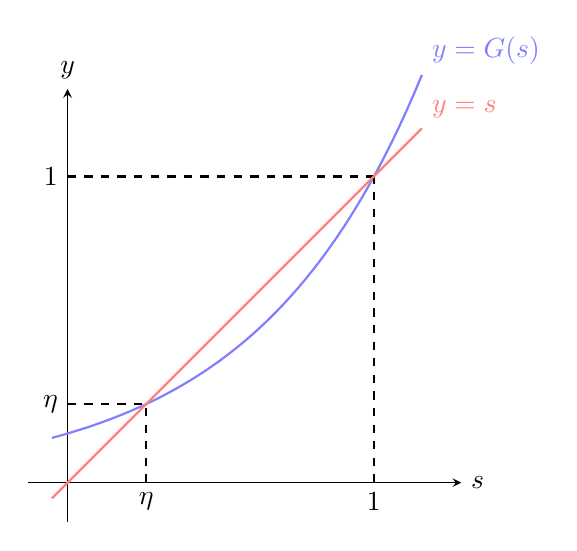
\begin{tikzpicture}
            \tzaxes(-0.5,-0.5)(5,5){$s$}{$y$}
            \def\Fx{1.6^(\x-1)}
            \tzfn[blue!50,thick]\Fx[-0.2:4.5]{$y=G(s)$}[ar]
            %\tzfn[blue!50]{\exp^(\x-1)}[0:2.5]{$y=G(\eta)$}[left]
            % \tzfn'[red]\Fx[-2:ln(2)/ln(2)]{$f(x)=\ln_2 x$}[ar] % inverse
            \draw[dashed,thick] (1,0)--(1,1);
            \node[below] at (1,0) {$\eta$};
            \node[left] at (0,1) {$\eta$};
            \node[below] at (3.89,0) {$1$};
            \node[left] at (0,3.89) {$1$};
            \draw[dashed,thick] (3.89,0)--(3.89,3.89);
            \draw[dashed,thick] (0,3.89)--(3.89,3.89);
            \draw[dashed,thick] (0,1)--(1,1);
            \tzfn[red!50,thick]{\x}[-0.2:4.5]{$y=s$}[ar]
        \end{tikzpicture}
        \caption{$\mu>1$}
        \label{figure:fig1}
    \end{figure}

A glance at Figure \ref{figure:fig1} (and a more analytical verification) tells us that
these intersections are coincident if $\mu = G^\prime(1) < 1$. On the other hand, 
if $\mu > 1$ then these two intersections are not coincident. In the special case when µ = 1 we need to distinguish
between the non-random case in which $\sigma^2 = 0, G(s) = s$, 
and $\eta = 0$, and the random case in which $\sigma^2 > 0, G(s) > s$ 
for $0 \leqslant s < 1$, and $\eta = 1$.
\end{proof}

\section{Characteristic functions}
\begin{definition}
    The \textbf{characteristic function} of $X$ is defined by 
    $$
    \phi(t)=E(e^{itX})=\int e^{itx}f(x)\mathrm{d}x = E(\cos tX)+i E(\sin tX).
    $$
\end{definition}
\begin{example}
    For $X\sim \operatorname{Cauchy}(1)$, its characteristic function is 
    \begin{align*}
    \int_{-\infty}^{+\infty} e^{itx}\frac{1}{\pi(1+x^2)}\mathrm{d}x &= 
    \int_{-\infty}^{+\infty}\frac{\cos tx}{\pi(1+x^2)}\mathrm{d}x\\
    \end{align*}
    To start the computation, we define a contour $\Gamma$ as a semicircle with diameter $[-R, R]$ on the real axis.
    Next, we define the function $f(z)=\dfrac{e^{itz}}{\pi(z^2+1)}=\dfrac{e^{itz}}{\pi(z+i)(z-i)}$.
    The pole of $f(z)$ lies exactly at $i$. At $z=i$:
    $$
    g(z)=(z-i)f(z)=\frac{e^{itz}}{\pi(z+i)}
    $$
    is analytic so the pole is simple and 
    $$
    \operatorname{Res}(f,i)=g(i)=\frac{e^{-t}}{2\pi i}.
    $$
    By Residue Theorem, 
    $$
    \int_\Gamma f(z)\mathrm{d}z = 2\pi i \operatorname{Res}(f,i) = e^{-t}.
    $$
    Send $R\to+\infty$, noting that 
    $$
    \int_{\mathbb{C}_{\mathbb{R}^+}} f(z)\mathrm{d}z = \left|
        \int_{\mathbb{C}_{\mathbb{R}^+}} \frac{1}{\pi} \frac{e^{itz}}{1+z^2} \mathrm{d}z
    \right|\leqslant \frac{1}{\pi} \frac{1}{R^2-1}\pi R \to 0.
    $$
    That is the arc of the semicircle has integration $0$ and finally
    $$
    \int_{\mathbb{R}}\frac{e^{itx}}{1+x^2}\frac{1}{\pi}\mathrm{d}x = e^{-|t|},\quad 
    \forall t \in \mathbb{R}.
    $$
\end{example}
\begin{figure}[h]
    \centering
    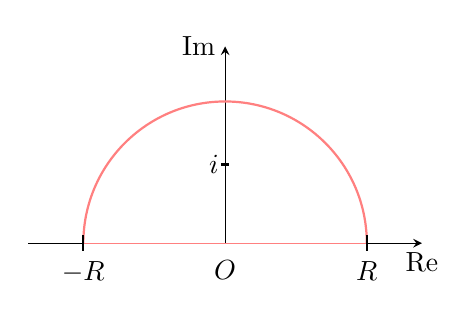
\begin{tikzpicture}
        \draw [->] (-2.5,0) -- (2.5,0)node[below]{Re};
        \draw [->] (0,0)node[below, yshift=-0.1cm]{$O$} -- (0,2.5)node[left]{Im};
        \draw [red!50,thick] (1.8,0) arc (0:180:1.8);
        \draw [red!50] (-1.8,0) -- (1.8,0);
        \draw [thick] (1.8,0.1) -- (1.8,-0.1)node[below]{$R$} (-1.8,.1) -- (-1.8,-0.1)node[below]{$-R$}
        (-0.05,1) -- (0.05,1)node[left]{$i$};
    \end{tikzpicture}
    \caption{The contour}
\end{figure}
\begin{theorem}\label{thm:thm2}
    The characteristic $\phi$ satisfies:
    \begin{enumerate}
        \item $\phi(0)=1, |\phi(t)|\leqslant 1$ for any $t\in\mathbb{R}$;
        \item $\phi$ is uniformly continuous;
        \item $\phi$ is positive semi-definite: for any $t_1,\cdots,t_n \in
        \mathbb{R}, z_1,\cdots,z_n\in\mathbb{C}$, 
        $$
        \sum_{i,j} \phi(t_i-t_j)z_i \overline{z_j}\geqslant 0.
        $$
    \end{enumerate}
\end{theorem}
Before proving the theorem, we first introduce some consequences in real analysis:
\begin{lemma}[Fatou]
    If $f_n\geqslant 0$, then 
    \begin{enumerate}
        \item $\displaystyle \int \liminf_{n\to\infty}f_n \mathrm{d}\mu \leqslant 
        \liminf_{n\to\infty} \int f_n\mathrm{d}\mu$;
        \item If $\sup f_n\leqslant f$, and $\displaystyle \int f\mathrm{d}\mu<+\infty$, then 
        $$
        \int \limsup_{n\to\infty}f_n\mathrm{d}\mu \geqslant \limsup_{n\to\infty} \int f_n\mathrm{d}\mu.
        $$
    \end{enumerate}
\end{lemma}
\begin{remark}
    In a probabilitic way: If $X_n\geqslant 0$, then 
    $$E(\liminf X_n)\leqslant \liminf E(X_n).$$
\end{remark}
\begin{proof}
    Note that $\liminf f_n = \sup_{m\geqslant 1}\inf_{n\geqslant m}f_n$, then 
    $g_m := \inf_{n\geqslant m}f_n \uparrow \liminf f_n$. By M.C.T., 
    $$
    \int \lim g_m \mathrm{d}\mu =
    \int \sup_{m\geqslant 1}g_m = \lim_{m\geqslant 1}g_m \mathrm{d}\mu.
    $$
    On the other hand, $\forall n\geqslant m$,
    $$
    \int g_m\mathrm{d}\mu \leqslant \int f_n \mathrm{d}\mu
    $$ 
    Taking $\inf$ with respect to $n$ on both sides, we obtain 
    $$
    \int g_m\mathrm{d}\mu \leqslant \inf_{n\geqslant m}\int f_n\mathrm{d}\mu.
    $$
    Send $m\to+\infty$, getting 
    $$
    \int \liminf f_n\mathrm{d}\mu =
    \lim \int g_m\mathrm{d}\mu \leqslant \liminf_{n\to\infty}\int f_n\mathrm{d}\mu 
    $$
\end{proof}
\begin{remark}
    \begin{enumerate}
        \item The equality may not be attained, i.e., there is $\{f_n\}$ such that 
        $\displaystyle \int \liminf f_n < \liminf \int f_n$:
        Let $f_n(x)=\mathds{1}_{[n,n+1]}(x)$, then $\liminf f_n = 0$.
        \item If $\{f_n\}$ are not non-negative, Fatou's Lemma may fail:
        Let $f_n(x)=-\mathds{1}_{[n,n+1]}(x)$.
    \end{enumerate}
\end{remark}

\begin{theorem}[Dominated Convergence Theorem(D.C.T)]
    Let $(\Omega, \mathcal{F},\mu)$ be a measure space. $\{f_n\},f$ are measurable functions 
    such that 
    \begin{enumerate}
        \item $f_n\to f$ a.e.;
        \item there is an integration function $g$ such that 
        $|f_n|\leqslant g,\forall n\geqslant1$, and $\displaystyle \int g \mathrm{d}\mu < +\infty$,  
    \end{enumerate}
    then $f$ is integrable with $\displaystyle \lim_{n\to\infty} f_n \mathrm{d}\mu 
        = \int f \mathrm{d}\mu$.
\end{theorem}
\begin{proof}
    Since $f_n+g\geqslant 0$, by Fatou, 
    $$
    \int \liminf (f_n+g)\leqslant \liminf \left[\int f_n + g\right]= 
    \liminf \int f_n + \int g,
    $$
    that is, 
    $$
    \int f \leqslant \liminf \int f_n.
    $$
    Similarly, $g-f_n\geqslant 0$ and by Fatou,
    $$ 
    \int \liminf (g-f_n)\leqslant \liminf \left[\int g- f_n\right] = \int g - \limsup 
    \int f_n
    $$
    that is 
    $$
    \limsup \int f_n \leqslant \int f.
    $$
    In conclusion 
    $$
    \limsup \int f_n \leqslant \int f \leqslant \liminf \int f_n 
    $$
    and this reduces to $\displaystyle \lim \int f_n = \int f$.
\end{proof}

\begin{theorem}[Bounded Convergence]
    For $\mu(\Omega)<+\infty$, if 
    \begin{enumerate}
        \item $f_n\to f$ a.e.;
        \item there is $K<+\infty$ such that $|f_n|\leqslant K$ a.e., then 
        $\displaystyle \int f_n = \int f$.
    \end{enumerate}
\end{theorem}
\begin{proof}
    Put $g=K$ and apply D.C.T..
\end{proof}

\begin{proof}[Proof of Theorem \ref{thm:thm2}]
    First prove 3. Note that 
    \begin{align*}
        \sum_{i,j} E(e^{i(t_i- t_j)X})z_i \overline{z_j}&= \sum_{i,j}E[e^{it_i X}
        e^{-it_j X}z_i\overline{z_j}]\\
        &= E\bigg[
            \sum_{i,j} e^{it_iX}z_i \cdot \overline{e^{it_jX}z_j}
        \bigg]\\
        &=E\biggl(\sum_{i}
            \bigg|
            e^{it_i X}z_i
            \bigg|^2
        \biggr)\geqslant 0.
    \end{align*}

    Continue with 2. Note that 
    \begin{align*}
        |\phi(t+h)-\phi(t)| &= |E(e^{i(t+h)X})-E(e^{itX})|=
        |E(e^{itX}(e^{ihX}-1))| \leqslant E(|e^{ihX}-1|)
    \end{align*}
    By Bounded Convergence, $\displaystyle \lim_{h\to 0} E(|e^{ihX}-1|)=0$.

    As for 1, one has 
    $$
    |\phi(t)|=\bigg| \int_{-\infty}^\infty e^{itx}f(x)\mathrm{d}x \bigg|
    \leqslant \int_{-\infty}^\infty |e^{itx}|f(x)\mathrm{d}x = 
    \int_{-\infty}^\infty f(x)\mathrm{d}x = \phi(0)=1.
    $$
\end{proof}

\begin{theorem}[Bachner]
    If $\phi$ satisfies statement 1,2 and 3 in Theorem \ref{thm:thm2}, then there is 
    a unique probability measure $P$ such that 
    $$
    \phi(t)=\int e^{itx}\mathrm{d}P.
    $$
\end{theorem}

\begin{theorem}
    \begin{enumerate}
        \item If $\phi^{(k)}(0)$ exists, then 
        $$
        \phi^k(0)=i^k E(X^k),
        $$
        from which we see 
        $$
        E(X)=\frac{\phi^\prime(0)}{i},\quad \operatorname{Var}(X)=
        -\phi^{\prime \prime}(0)+(\phi^\prime(0))^2.
        $$
        \item If $\phi^{(k)}(0)$ exists, then 
        $
        \begin{cases}
            E|X^k|< \infty, & \text{if } k \text{ is  even},\\
            E|X^{k-1}| < \infty, & \text{if } k \text{ is odd}.
        \end{cases}
        $
        \item If $E(|X|^k)<+\infty$, then 
        $$
        \phi(t)=\sum_{j=0}^k \frac{(it)^j}{j!} E(X^j)+o(t^k).
        $$
    \end{enumerate}
\end{theorem}

\begin{theorem}
    If $X$ and $Y$ are independent, then $\phi_{X+Y}(t)
    =E[e^{it(X+Y)}]=\phi_X(t)\phi_Y(t)$.
\end{theorem}
\begin{lemma}
    If $Y=aX+b$ for some $a,b\in\mathbb{R}$, then 
    $\phi_Y(t)=e^{itb}\phi_X(at)$.
\end{lemma}
\begin{definition}
    The \textbf{joint characteristic function} of $X$ and $Y$ is given by 
    $$
    \phi(s,t)=E[e^{isX+itY}].
    $$
\end{definition}
\begin{theorem}
    $X$ and $Y$ are independent $\iff$ $\phi(s,t)=\phi_X(s)\phi_Y(t)$.
\end{theorem}

\begin{theorem}[Analytic extension of $M(t)$]
    Let $M(t) = E(e^{tX}), t \in \mathbb{R}$, and $\phi(t) = E(e^{itX}), t\in\mathbb{C}$, 
    be the moment generating function and characteristic function, respectively, 
    of a random variable $X$. For any $a > 0$, the following three statements are equivalent:
    \begin{enumerate}
        \item $|M(t)|<+\infty$ for $|t|<a$;
        \item $\phi(z)=E(e^{tX})$ is analytic in the strip $|\operatorname{Re}(z)|<a$;
        \item The moments $m_k=E(X^k), k\in\mathbb{N}$ exists and 
        $\displaystyle \lim_{k\to\infty}\left(
            \dfrac{m_k}{k!}
        \right)^{\frac{1}{k}}\leqslant \dfrac{1}{a}$. 
    \end{enumerate} 
    If any of these conditions hold for $a > 0$, the power series expansion for $M(t)$ may be
extended analytically to the strip $|\operatorname{Im}(t)| < a$, resulting in a function $M$ with the property that $\phi(t) = M(it)$.
\end{theorem}

\section{Common characteristic functions}
\begin{example}[(Delta Measure)] We have $f_X(a)=1$ and 
    $\phi(t)=E(e^{itX})=e^{iat}$.
\end{example}
\begin{example}[(Bernoulli$(p)$)]
    $\phi(t)=E^{e^{itX}}=pe^{it}+q$.
\end{example}
\begin{example}[(Binomial$(n,p)$)]
    Note the decompositon $X=Y_1+\cdots+Y_n$ with $Y_i\sim \text{i.i.d. } \operatorname{Bernoulli}(p)$.
    Then 
    $$
    E(e^{itX})=(E(e^{itY_1}))^n = (pe^{it}+q)^n.
    $$
\end{example}
\begin{example}[(Poisson$(\lambda)$)]
    Recall that $f(k)=\dfrac{\lambda^k}{k!}e^{-\lambda}$, then 
    $$
    \phi(t)=E(e^{itX})=\sum_k e^{itk}\frac{\lambda^k}{k!}e^{-\lambda}=e^{\lambda e^{it}-\lambda}.
    $$
\end{example}
\begin{example}[(Exponential$(\lambda)$)]
    Recall that $f(x)=\lambda e^{-\lambda x}\mathds{1}_{[0,+\infty)}(x)$. Then 
    $$
    \phi(t)=E(e^{itX}) = \int_0^{+\infty} e^{itx}\lambda e^{-\lambda x}\mathrm{d}x = 
    \frac{\lambda}{\lambda - it}.
    $$
\end{example}
\begin{example}[(Normal)]
    $\phi(t)=E(e^{itX})=\displaystyle \int_{\mathbb{R}}e^{itx}e^{-\frac{x^2}{2}}\mathrm{d}x$
    whereas 
    $M(t)=E(e^{tX})=e^{\frac{1}{2}t^2}$. By analytic extension, $\phi(t)=
    M(it)=e^{-\frac{1}{2}t^2}$.
    If $Y\sim \mathcal{N}(\mu,\sigma^2)$, then $Y=\mu + \sigma X$ for some $X\sim 
    \mathcal{N}(0,1)$ and 
    $$\phi_Y(t)=e^{i\mu t} E(e^{i\sigma t X})= 
    e^{i\mu t-\frac{1}{2}\sigma^2 t^2}.$$ 
\end{example}
\begin{note}
    Indeed, for $X\sim \mathcal{N}(0,1)$, note that 
    $$
    \phi(t)=\frac{1}{\sqrt{2\pi}}\int_{-\infty}^{\infty}e^{itx}e^{-\frac{x^2}{2}}\mathrm{d}x=
    \frac{1}{\sqrt{2\pi}}\int_{-\infty}^{\infty} \sum_{n=0}^\infty \frac{(itx)^n}{n!}
    e^{-\frac{x^2}{2}}\mathrm{d}x = 
    \sum_{n=0}^\infty \frac{(it)^n}{n!}\biggl[
        \frac{1}{\sqrt{2\pi}}\int_{-\infty}^\infty x^n e^{-\frac{x^2}{2}}\mathrm{d}x
    \biggr]
    $$
    Recall that 
    $E(X^n)=
    \begin{cases}
    0, & n=2m-1,\\
    (2m-1)!!=\dfrac{(2m)!}{2^m\cdot m!}, & n = 2m.    
    \end{cases}$
    Thus 
    $$
    \phi(t)=\sum_{m=0}^\infty \frac{(it)^{2m}}{(2m)!}\cdot \frac{(2m)!}{2^m\cdot m!}=
    \sum_{m=0}^\infty \biggl(
        -\frac{t^2}{2}
    \biggr)^m\frac{1}{m!}=e^{-\frac{t^2}{2}}.
    $$
\end{note}
\begin{example}
    $(X_1,\cdots,X_n)\sim \mathcal{N}(0,V)$ if and only if 
    $\operatorname{Cov}(X_i,X_j)=V_{ij}$. Their joint density funciton is 
    $$
    f(x_1,\cdots,x_n)=\frac{1}{\sqrt{(2\pi)^n \det V}}e^{-\frac{1}{2}x^T V^{-1} x}.
    $$
    For $t_1,\cdots,t_n \in \mathbb{R}$, the joint characteristic function is 
    $$
    E(e^{i(t_1X_1+\cdots+t_nX_n)})=\frac{1}{\sqrt{(2\pi)^n \det V}}\int 
    e^{i(t_1x_1+\cdots+t_nx_n)}e^{-\frac{1}{2}x^T V^{-1} x}\mathrm{d}x.
    $$
    Consider the diagonalization of $V^{-1}$: there is orthogonal matrix $B$ 
    and diagonal matrix $\Lambda = \operatorname{diag}(\lambda_1,\cdots,\lambda_n)$ such that 
    $B^TV^{-1}B =\Lambda$. Let $x=By$, then 
    \begin{align*}
        x^{T}V^{-1}x&=y^{T}B^TV^{-1}By = y^T \Lambda y = \sum \lambda_i y_i^2, \\
        \phi(t)&= e^{-\frac{1}{2}t^T V t}.
    \end{align*}
    Alternatively, let $Y=(Y_1,\cdots,Y_n)=AX$, then $Y\sim\mathcal{N}(0,\lambda)$ with 
    $Y_1,\cdots,Y_n$ being independent normal. Thus 
    $$
    t_1X_1+\cdots+t_nX_n = t^T X = t^TA^T Y
    $$ 
    is a linear transformation of independent normal and is therefore normal. Therefore,
    $$
    E(t_1X_1+\cdots+t_nX_n)=0,\quad \operatorname{var}(t_1X_1+\cdots+t_nX_n)=
    \sum_{i,j}t_it_j \operatorname{cov}(X_i,X_j)=\sum_{i,j}t_iV_{ij}t_j = t^TVt.
    $$
    Finally,
    $$
    E[e^{i(t_1X_1+\cdots+t_nX_n)}] = e^{-\frac{1}{2}\operatorname{var}(t_1X_1+\cdots+t_nX_n)}
    =e^{-\frac{1}{2}t^T V T}.
    $$
\end{example}
\begin{example}[(Geometric)]
    The characteristics function of geometric distribution is
$$
\begin{aligned}
\phi(t) & =E\left(e^{i t X}\right) =\sum_{x=0}^{\infty} e^{i t x} P(X=x) \\
&=\sum_{x=1}^{\infty} e^{i t x} q^{x-1} p
  =pq^{-1} \bigg(\sum_{x=0}^{\infty}(q e^{i t})^x-1\bigg)\\
& =pe^{it}\left(1-q e^{i t}\right)^{-1} 
\end{aligned}
$$
by noting that $\displaystyle \sum_{x=0}^{\infty} q^x=(1-q)^{-1}$.
\end{example}
\begin{example}[(Pascal)]
    The Pascal distributed $X$ has density function 
    $$
    f(k)=\binom{k-1}{r-1}p^r(1-p)^{k-r},\quad k=r,r+1,\cdots.
    $$
    One can decompose $X$ into $r$ i.i.d. geometric$(p)$ random variables, i.e.,
    $X=X_1+X_2+\cdots+X_r$. Then 
    $$
    \phi_X(t)=\prod_{j=1}^r \phi_{X_j}(t)=\biggl(
        \frac{pe^{it}}{1-qe^{it}}
    \biggr)^r.
    $$
\end{example}

\section{Inversion and continuity}
Recall $\phi(x)=\displaystyle \dfrac{1}{2\pi}\int_{-\infty}^\infty 
e^{itx}f(x)\mathrm{d}x$. Then by 
Fourier inversion theorem, the density function is 
\begin{equation}\label{inversion}
f(x)=\dfrac{1}{2\pi}\int_{-\infty}^\infty e^{-itx}\phi(t)\mathrm{d}t
\end{equation}
at every point $x$ such that $f$ is differentiable.
\begin{example}[(Revisit to Cauchy distribution)]
    Knowing $\phi(t)=e^{-|t|}$ and apply (\ref{inversion}), we get 
    \begin{align*}
        f(x)&=\frac{1}{2\pi}\int_{-\infty}^\infty e^{-ixt}\cdot e^{-|t|}\mathrm{d}t\\
        &=\frac{1}{2\pi}\int_0^\infty e^{-(1+ix)t}\mathrm{d}t+\frac{1}{2\pi}\int_{-\infty}^0
        e^{(1-ix)t}\mathrm{d}t\\
        &=\frac{1}{2\pi}\biggl(
            \frac{1}{1+ix}+\frac{1}{1-ix}
        \biggr)=\frac{1}{\pi(1+x^2)}.
    \end{align*}
    Thus $X$ is Cauchy distributed.
\end{example}
\begin{theorem}[Inversion]
    Let $X$ have the distribution $F$ and characteristic fucntion $\phi$. Let 
    $$
    \overline{F}(x)=\frac{1}{2}(F(x)+\lim_{y\uparrow x}F(y)).
    $$
    Then for any $a<b$, 
    $$
    \overline{F}(b)-\overline{F}(a)=\lim_{N\to+\infty} \int_{-N}^N 
    \frac{e^{-iat}-e^{-ibt}}{2\pi i t}\phi(t)\mathrm{d}t.
    $$
\end{theorem}
\begin{corollary}
    If $\phi_X(t)=\phi_Y(t)$, then $F_X=F_Y$.
\end{corollary}
\begin{proof}
    Apply Inversion Theorem with $a=-\infty$: $\overline{F}_X(b)=\overline{F}_Y(b)$.
    For any $x\in\mathbb{R}$, we use the right continuity of $F_X$ and $F_Y$. Take 
    $b_n\downarrow x$ such that $F_X, F_Y$ are continuous at $b_n$. Then 
    $$
    \overline{F}_X(b_n)=F_X(b_n)=F_y(b_n)=\overline{F}_Y(b_n),
    $$
    implying that $F_X(x)=F_Y(x)$.
\end{proof}
\begin{theorem}[Uniqueness]
    Distribution function is uniquely determined by the characteristic function.
\end{theorem}
\begin{example}
    We now have a more elegant way to demonstrate the sum of two independent Gaussian
    r.v.s is still Gaussian: suppose that $X\sim \mathcal{N}(\mu_1,\sigma_1^2),
    Y\sim \mathcal{N}(\mu_2,\sigma_2^2)$ are independent, their characteristic functions 
    are 
    $$
    \phi_X(t)=e^{it\mu_1-\frac{1}{2}\sigma_1^2t^2},\quad 
    \phi_Y(t)=e^{it\mu_2-\frac{1}{2}\sigma_2^2t^2}.
    $$
    Use independence,
    $$
    \phi_{X+Y}(t)=\phi_X(t)\cdot \phi_Y(t)=e^{it(\mu_1+\mu_2)-\frac{1}{2}(\sigma_1^2+
    \sigma_2^2)t^2}
    $$
    From Uniqueness Theorem, one deduces that $X+Y \sim \mathcal{N}(\mu_1+\mu_2,\sigma_1^2+
    \sigma_2^2)$.
\end{example}
\begin{exercise}
    Let $X$ be a random variable with density function $f(x)$ and 
    characteristic function $\phi(t)$. Show that $f(x)$ is even if and only if 
    $\phi(t)$ is real and even.
\end{exercise}
\begin{proof}
    $\Longleftarrow$. We now have $\phi_X(t)=\phi_X(-t)=\phi_{-X}(t)$, i.e.,
    $X$ and $-X$ have the same characteristic function. Thus they have the same 
    distribution and $f_X(x)=f_{-X}(x)=f_X(-x)$.

    $\Longrightarrow$. We now deduce that $X$ and $-X$ have the same 
    distribution (and the same characteristic function) from $f(x)=f(-x)$. Furthermore,
    note that $\phi_{-X}(t)=\phi_{X}(-t)=\overline{\phi_X(t)}$, implying that $\phi(t)$
    is indeed real and even. 
\end{proof}

\begin{definition}
    Let $\{X_n\}_{n\geqslant 1}$ and $Y$ be random variables, then we say $X_n$ 
    \textbf{converges in distribution} to $Y$, denoted by $X_n \overset{D}{\longrightarrow}Y$,
    if $\displaystyle \lim_{n\to\infty} P(X_n\leqslant x)=P(Y\leqslant x)=F_Y(x)$ for all $x$ such that $F_Y$ is 
    continuous at $x$.
\end{definition}
\begin{remark}
    The continuity assumption at $x$ is to deal with discrete random variables:
    Let $X_n = x_n \downarrow x := X$. Then $F_{X_n}(x)=0$ but $F_X(x)=1$.
\end{remark}

\begin{theorem}[Continuity]
    Suppose a sequence of r.v.s $\{X_n\}_{n\geqslant 1}$ have corresponding characteristic
    funnction $\{\phi_n\}_{n\geqslant 1}$. 
    \begin{enumerate}
        \item If $X_n \overset{D}{\longrightarrow}X$, then $\phi_n(t)\to \phi(t)$ for all $t$;
        \item Conversely, if $\phi_n(t)\to\phi(t)$ for all $t$, 
        and $\phi(t)$ is continuous at $t=0$,
        then $\phi$ is the characteristic function of some random variable $X$ such that 
        $X_n \overset{D}{\longrightarrow}X$.
    \end{enumerate}
\end{theorem}
\begin{theorem}[Weak law of large numbers]
    Let $X_1,X_2,\cdots,X_n$ be a sequence of independent r.v.s such that $E(X_i)=\mu,
    i=1,2,\cdots,n$.
    Then $S_n=X_1+\cdots+X_n$ satisfies $\dfrac{1}{n}S_n \overset{D}{\longrightarrow}\mu$.
\end{theorem}
\begin{proof}
    Let $\phi_n$ be the characteristic function of $\dfrac{1}{n}S_n$. 
    $$
    \phi_n(t)=E(e^{it\frac{1}{n}(X_1+\cdots+X_n)})=[E(e^{i\frac{t}{n}X_1})]^n 
    \overset{E(X_1)<\infty}{=}\left(
        1+i \frac{t}{n}E(X_1)+O\left(\frac{t}{n}\right)
    \right)^n
    $$
    and 
    $$
    \lim_{n\to\infty}\phi_n(t)=\lim_{n\to\infty}\left(
        1+i\frac{t}{n}\mu+O\left(\frac{t}{n}\right)
    \right)^n = e^{it\mu}.
    $$
    By continuity theorem, $\dfrac{1}{n}S_n\overset{D}{\longrightarrow}\mu$.
\end{proof}
\begin{note}
    The ``independent'' restriction indeed can be weakened to ``uncorrelated'':
    Let $X_1,X_2,\cdots,X_n$ be a sequence of uncorrelated r.v.s 
    with the same distribution such that $E(X_iX_j)=E(X_i)E(X_j),E(X_i^2)<\infty,
    E(X_i)=\mu, i,j=1,2,\cdots,n$.
    Then $S_n=X_1+\cdots+X_n$ satisfies 
    $$\overline{X_n}:=\dfrac{1}{n}S_n \overset{P}{\longrightarrow}\mu.$$
    In fact, $\dfrac{1}{n}\displaystyle \sum_{i=1}^n
        X_i \overset{L^2}{\longrightarrow} \mu$:
        $$
        E\left(
            \bigg(\frac{1}{n}\sum_{i=1}^n X_i-\mu\bigg)^2
        \right)= 
        \frac{1}{n^2}\sum_{i,j=1}^nE[(X_i-\mu)(X_j-\mu)]=\frac{1}{n^2}
        \sum_{i=1}^n \operatorname{var}(X_i) \leqslant \frac{c}{n}
        $$
        a.s. as $n\to \infty$.
\end{note}

\begin{theorem}[Strong law of large numbers]
    Let $X_1,\cdots,X_n:\Omega \to \mathbb{R}$ be i.i.d. with mean $\mu$ and 
    $E(|X_1|)<\infty$, then $\dfrac{1}{n} S_n \to \mu$ a.s..
\end{theorem}

\begin{example}[(Monte Carlo simulations: Numerically stimulate $\pi$)]\label{eg:eg6}
    We generate $U_i,V_i(i=1,2,\cdots,r)$ 
    which are independent and uniformly $[-1,1]$ distributed. We stipulate
    that 
    $$X_i=
    \begin{cases}
        1, & U_i^2+V_i^2 \leqslant 1\\
        0,& \text{otherwise} 
    \end{cases}
    $$ 
    Then $X_i$ is Bernoulli and $E(X_i)=P(X_i=1)=\dfrac{\pi}{4}$. By law of large numbers,
    $$
    \overline{X_n}:=\frac{1}{n}\sum_{i=1}^n X_i \overset{P}{\longrightarrow} E(X_i)=
    \frac{\pi}{4}.
    $$
\end{example}
\begin{definition}
    Given r.v.s. $\{X_n\}$, a confident interval for the theoretical mean $\mu$ with 
    \textbf{confident level $\beta\%$} is an interval of length $2\varepsilon$ such that
    $$
    P[\mu\in(\overline{X_n}-\varepsilon,\overline{X_\varepsilon}+\varepsilon)]\geqslant
    \beta\%.
    $$ 
\end{definition}
\begin{example}
    What is the smallest $n$ such that one obtains a four-digit accuracy of $\pi$ with 
    confident level $99\%$? 
\end{example}
\begin{proof}[Solution]
    Note that the stimulation in Example \ref{eg:eg6} is $\dfrac{\pi}{4}$ and thus 
    the error $\varepsilon$ here is $\dfrac{1}{4000}$ and the confident level is
    $\beta=99\%$. 
    We look for $n$ such that 
    $$
    P\bigg(\bigg|\overline{X_n}-\frac{\pi}{4}\bigg|>\frac{1}{4000}\bigg)\leqslant 1\% \eqno{(\clubsuit)}
    $$
    Note that $X_i$ is Bernoulli$(p)$ and $\operatorname{Var}(X_i)=p(1-p)
    \leqslant \dfrac{1}{4}$. From Chebychev,
    $$
    P\bigg(\bigg|\overline{X_n}-\frac{\pi}{4}\bigg|>\frac{1}{4000}\bigg)\leqslant 
    4000^2\cdot \operatorname{Var}(\overline{X_n})=4000^2 \frac{1}{n^2}
    \sum_{i=1}^n \operatorname{Var}(X_i) \leqslant \frac{4000^2}{n}\cdot \frac{1}{4}.
    $$
    Thus if $n\geqslant 400\times 10^6$, $(\clubsuit)$ automatically holds.
\end{proof}
\begin{example}[(Revisit to coupon collector)]
    $\Omega=\{1,2,\cdots,n\}$ and $X_n$ be i.i.d. uniformly $\{1,2,\cdots,n\}$.
    We use $T_i=\inf \{n:|\{X_1,X_2,\cdots,X_n\}|=i\}$, the 1st time to collect 
    $i$ different coupons. We have showed that $\dfrac{E(T_n)}{n\ln n}\to 1$.
    Now I claim that 
    $$
    \frac{T_n}{\ln n}\overset{P}{\longrightarrow} 1.
    $$

    Indeed, note that $T_n=\displaystyle \sum_{i=1}^n (T_i-T_{i-1})$ with 
    $(T_i-T_{i-1}) \sim \operatorname{Geo}\biggl(
        1-\dfrac{i-1}{n}
    \biggr)$.
    We already showed that $E(T_n)=n\ln n+o(n)$ and 
    \begin{align*}
    \operatorname{Var}(T_n)&=\sum_{i=1}^n (T_i-T_{i-1})=
    \sum_{i=1}^n\frac{\frac{i-1}{n}}{(1-\frac{i-1}{n})^2}
    \leqslant
    \sum_{i=1}^n\frac{1}{(1-\frac{i-1}{n})^2}\\
    &=n^2 \sum_{m=1}^n \frac{1}{m^2}\leqslant cn^2.
    \end{align*}
    In particular, $\dfrac{\operatorname{Var}(T_n)}{E(T_n)^2}\to 0$. By 
    extension of WLLN, 
    $$
    \frac{T_n-E(T_n)}{n\ln n}\overset{P}{\longrightarrow} 0
    $$
    and thus $\dfrac{T_n}{n\ln n}\overset{P}{\longrightarrow} 1$.
\end{example}
\begin{note}
    Let $T_n=\displaystyle \sum_{i=1}^n X_i$ for every sequence $\{a_n\}$ such that 
    $\dfrac{\operatorname{Var}(T_n)}{a_n^2}\to 0$ as $n\to\infty$. We have 
    $\dfrac{T_n-E(T_n)}{a_n}\overset{P}{\longrightarrow} 0$.
\end{note}

\begin{exercise}
    Use characteristic function to prove the Central Limit Theorem:
    \begin{theorem}
        Let $\{X_i\}$ be i.i.d. r.v.s with $E(X_i)=0$ and $E(X_i^2)=1$.
        Assume $E(X_i^3)<+\infty$, then 
        $$
        \frac{1}{\sqrt{n}}\sum_{i=1}^n X_i
        \overset{D}{\longrightarrow} \mathcal{N}(0,1).
        $$
    \end{theorem}
\end{exercise}
\begin{proof}
    Compute the characteristic function:
    \begin{align*}
        \phi_n(t) &= E\bigg[e^{i\frac{t}{\sqrt{n}}\sum_{i=1}^n X_i}\bigg] =
        \bigg(E\bigg[e^{i\frac{t}{\sqrt{n}}X_1}\bigg]\bigg)^n \\
        &=\left[
            1+i\frac{t}{\sqrt{n}}E(X_1)-\frac{1}{2}\frac{t^2}{n}E(X_1^2)+O\left(
                \frac{t^3}{n^{3/2}}
            \right)
        \right]^n\\
        &\overset{n\to\infty}{\longrightarrow} e^{-\frac{t^2}{2}}.
    \end{align*}
\end{proof}

\chapter{Convergence or random variables}
\section{Different modes of convergence}
\begin{definition}
    Let $\{X_n\}_{n\geqslant 1}$ be random variables in $(\Omega,\mathcal{F},\mu(\text{ or }
    P))$. Then 
    \begin{enumerate}
        \item We say $X_n$ converges to $X$ almost surely (a.s.) if $P(\{\omega:\displaystyle
        \lim_{n\to\infty}X_n(\omega)=X(\omega)\})=1$;
        \item We say $X_n$ converges to $X$ in probability, denoted as $X_n\overset{P}{\longrightarrow}
        X$ if for any $\varepsilon>0$, $P(|X_n-X|>\varepsilon)\to 0$ as $n\to\infty$;
        \item We say $X_n$ converges to $X$ in the $p$th moment if $E(|X_n|^p)<+\infty$ for any $n\in\mathbb{N}$
        and $E(|X_n-X|^p)\to 0$ as $n\to\infty$;
        \item We say $X_n$ converges to $X$ almost uniformly if for all
        $\varepsilon>0$, there is $E\in\mathcal{F}:\mu(E)<\varepsilon$ such that 
        $f_n \rightrightarrows f$ on $E^c$;
        \item We say $X_n$ converges in distribution to $Y$, denoted by $X_n \overset{D}{\longrightarrow}Y$,
        if $\displaystyle \lim_{n\to\infty} P(X_n\leqslant x)=P(Y\leqslant x)=F_Y(x)$ for all $x$ such that $F_Y$ is 
        continuous at $x$.
    \end{enumerate}
\end{definition}
\begin{remark}
    \begin{enumerate}
    \item $X_n \to X$ in $p$th moment implies $X_n \to X$ in probability:
    for any $\varepsilon>0$, by Chebychev 
    $$
    P(|X_n-X|>\varepsilon)\leqslant \frac{E(|X_n-X|^p)}{\varepsilon^p} \to 0.
    $$
    \item $X_n\to X$ a.e. implies $X_n\to X$ in probability.
    \item $X_n \to X$ a.s. does not imply $X_n \to X$ in $p$th moment:
    consider $f_n(x)=\mathds{1}_{[n,n+1)}(x)$ with $f_n \to 0$ a.s. but 
    $f_n$ is not convergent to $0$ in probability or $p$th moment.
    \item $X_n \to X$ in $p$th moment does not imply $X_n \to X$ a.s.
    \end{enumerate}
\end{remark}
\begin{proposition}\label{prop:prop4}
    $f_n \to f$ almost uniformly if and only if for all $\varepsilon>0$,
    $\displaystyle \lim_{m\to\infty} \mu\biggl(
        \bigcup_{n\geqslant m}\{|f_n-f|>\varepsilon\}
    \biggr)=0 $.
\end{proposition}
\begin{proof}
    $\Longrightarrow$. If $f_n \to f$ a.u., then for all $\delta>0$, there is $E$
    with $\mu(E)<\delta$ such that $f_n \rightrightarrows f$ on $E^c$. Thus 
    for all $\varepsilon>0$, there is $m\in\mathbb{N}$ such that for all $n\geqslant m$,
    one has $|f_n-f|< \varepsilon$ on $E^c$. For such $m$, note that 
    $\displaystyle \bigcup_{n\geqslant m} \{|f_n-f|>\varepsilon\}\subseteq E$ and thus 
    $$
    \mu \biggl(
        \bigcup_{n\geqslant m}\{|f_n-f|>\varepsilon\} \biggr) \leqslant \mu(E)<\delta
    $$ 
    Send $\delta \to 0$, we have $\displaystyle \lim_{m\to\infty} \mu\biggl(
        \bigcup_{n\geqslant m}\{|f_n-f|>\varepsilon\}
    \biggr)=0$.

    $\Longleftarrow$. Suppose that for any $k\geqslant 1$, we have 
    $\displaystyle \lim_{m\to\infty} \mu\biggl(
        \bigcup_{n\geqslant m}\bigg\{|f_n-f|>\dfrac{1}{k}\bigg\}=0
    \biggr)$. For any $\delta>0$, we can find $m=m(\delta,k)$ such that 
    $ \mu\biggl(\displaystyle
        \bigcup_{n\geqslant m}\bigg\{|f_n-f|>\dfrac{1}{k}\bigg\}
    \biggr)\leqslant \dfrac{\delta}{2^k}$. Define 
    $$
    E= \bigcup_{k\geqslant 1}\bigcup_{m\geqslant m(\delta,k)}
    \biggl(
        \bigg\{|f_n-f|>\dfrac{1}{k}\bigg\}
    \biggr)
    $$
    Then $\mu(E)<\delta$ and $f_n \rightrightarrows f$ on $E^c$.
\end{proof}

\begin{corollary}
    \begin{enumerate}
        \item $f_n \to f$ a.u. $\Longrightarrow$ $f_n \to f$ in measure;
        \item If $\mu(\Omega)<+\infty$, then $f_n\to f$ a.e. $\Longrightarrow$ 
        $f_n\to f$ in probability (or in measure).
    \end{enumerate}
\end{corollary}
\begin{theorem}
    $X_n \to X$ in probability implies $X_n \to X$ in distribution. 
\end{theorem}
\begin{proof}
    Note that for all $a\in\mathbb{R},\varepsilon>0$,
    $$
    \{X_n\leqslant a\}\subseteq \{X\leqslant a+\varepsilon\} \cup \{|X_n-X|>\varepsilon\}.
    $$ 
    Thus 
    $$
    P(X_n\leqslant a)\leqslant P(X\leqslant a+\varepsilon)+P(|X_n-X|>\varepsilon)
    $$
    and 
    similarly, $\{X\leqslant a-\varepsilon\}\subseteq \{X_n \leqslant a\}\cup 
    \{|X_n-X|>\varepsilon\}$ and 
    $$
    P(X\leqslant a- \varepsilon)\leqslant P(X_n\leqslant a)+P(|X_n-X|>\varepsilon)
    $$
   Using $X_n \to X$ in probability and sending $n\to\infty$, we have 
   $
   \begin{cases}
    \limsup P(X_n\leqslant a)\leqslant P(X\leqslant a+\varepsilon)=F_X(a+\varepsilon),\\
    \liminf P(X_n\leqslant a)\geqslant P(X\leqslant a-\varepsilon)=F_X(a-\varepsilon).
   \end{cases}
   $
   If $a$ is continuity point of $F_x$, then one can send $\varepsilon \to 0$ to conclude 
   $\lim P(X_n\leqslant a) = P(X\leqslant a)$.
\end{proof}
However, convergence in distribution does not imply convergence in probability:
\begin{example}
    Let $X$ have probability denstiy function
    $$
    P(X=-1)=\frac{1}{2},\quad P(X=1)=\frac{1}{2}
    $$
    and set $X_n=-X$. Note that $X_n$ and $X$ have the same distribution and hence 
    $X_n \overset{D}{\longrightarrow} X$. However, for $0<\varepsilon<2$, one has 
    $$
    P(|X_n-X|\geqslant \varepsilon)=P(2|X|\geqslant \varepsilon)=1 \nrightarrow 0,
    $$
    that is $X_n$ does not converge to $X$ in probability.
\end{example}
\begin{conclusion}
    \begin{enumerate}
        \item $f_n\to f$ almost uniformly $\Longrightarrow$ $f_n\to f$ a.e.
        \item If $\mu(\Omega)<+\infty$, then $f_n\to f$ a.e. $\iff$ $f_n \to f$ 
        a.u. (Egorov).
        \item $f_n \to f$ in probability(measure) $\Longrightarrow$ $f_n \to f$ in  
        distribution.
    \end{enumerate}
\end{conclusion}

\begin{figure}[htbp]
    \centering
    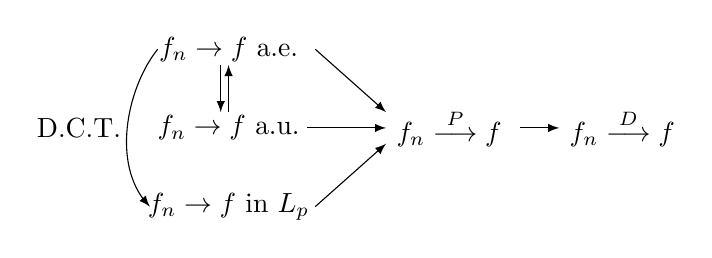
\begin{tikzpicture}[>=Stealth]
        % \draw[-latex] (3,1.6) -- (3,0);
        \draw[-latex] (4,2) -- (5,2);
        \draw[-latex] (4.1,1) -- (5,1.8);
        \draw[-latex] (4.1,3) -- (5,2.2);
        \draw[-latex] (3,2.2) -- (3,2.8);
        \draw[-latex] (6.7,2) -- (7.2,2);
        \draw[-latex] (2.9,2.8) -- (2.9,2.2);
        % \draw[-latex] (3,3) -- (3,1); 
        
        \node (G) at (3,3) {$f_n\to f$ a.e.}; 
        \node (A) at (3,2) {$f_n\to f$ a.u.};
        \node (B) at (3,1) {$f_n \to f$ in $L_p$};
        \node (C) at (5.8,2) {$f_n \overset{P}{\longrightarrow} f$};
        \node (E) at (8,2) {$f_n \overset{D}{\longrightarrow} f$};
        % \node (D) at (2.6,0.9) {$p$};
        % \node (E) at (4.2,2.3) {$f$};
        % \node (F) at (4.5,0.7) {$\bar{f}$};
        \path (2.1,3) coordinate(c1)
(1.7,2.5) coordinate(c2)
(1.5,1.5) coordinate(c3)
(2,1) coordinate(c4);
        \draw [-latex] (c1) .. controls (c2) and (c3)
.. (c4);
\node (D) at (1.1,2) {D.C.T.};
\end{tikzpicture}
\caption{Different convergence}
\label{figure:fig2}
\end{figure}

\begin{example}
    For $X_n \sim \operatorname{Cauchy}(n)$, i.e., $f_n(x)=\dfrac{n}{(1+n^2x^2)\pi}$, 
    we have $X_n \overset{D}{\longrightarrow} 0$.
\end{example}
\begin{proof}
    In fact, $X_n \overset{P}{\longrightarrow} 0$: $\forall \varepsilon>0$, 
    $$
    P(|X_n|>\varepsilon)=2\int_\varepsilon^\infty \frac{n}{(1+n^2x^2)\pi} \mathrm{d}x
    =2 \left(
        1-\frac{2}{\pi}\arctan n\varepsilon
    \right)
    \overset{n\to\infty}{\longrightarrow}0
    $$
\end{proof}

\begin{proposition}
    $X_n \overset{P}{\longrightarrow}X \iff$ for any subsequence $\{X_{n_l}\}$, there 
    is a further subsequence $\{X_{n_k}\}$ such that 
    $X_{n_k} \longrightarrow X$ a.u. (or a.s.).
\end{proposition}
\begin{proof}
    $\Longrightarrow$. For any subsequence $\{X_{n_l}\}$, we have
    $X_{n_l} \overset{P}{\longrightarrow}X$ and thus 
    $\forall k \geqslant 1$, $P\bigg(
        |X_{n_l}-X|>\dfrac{1}{k}
    \bigg)\to 0$ as $n_l \to \infty$. Choose $n_k(>n_{k-1})$ such that 
    $P\bigg(\displaystyle \bigcup_{k\geqslant m}
        |X_{n_k}-X|>\dfrac{1}{k}
    \bigg)\leqslant \dfrac{1}{2^{m-1}}$. For all $\varepsilon>0$,
    $$
    P\bigg(\displaystyle \bigcup_{k\geqslant m}
        |X_{n_k}-X|>\varepsilon
    \bigg)\leqslant 
    P\bigg(\displaystyle \bigcup_{k\geqslant m}
        |X_{n_k}-X|>\dfrac{1}{k}
    \bigg)\leqslant \frac{1}{2^{m-1}}
    \overset{m\to\infty}{\longrightarrow}0.
    $$
    Then by Proposition \ref{prop:prop4}, we obtain $X_{n_k}\to X$ a.u..

    $\Longleftarrow$. Prove by contradiction. If $X_n$ does not converge to $X$ in probability,
    there is $\varepsilon_0>0,\sigma_0>0$ and a subsequence $\{n_i\}$ such that 
    $$
    \lim_{i\to\infty}P(|X_{n_i}-X|>\varepsilon_0)\geqslant \sigma_0  \eqno{(\diamondsuit)}
    $$
    But by the condition, there is $\{n_{i_j}\}$ such that 
    $X_{n_{i_j}}\to X(j\to\infty)$ a.s., implying $X_{n_{i_j}}$ converges to $X$
    in probability, contradicting $(\diamondsuit)$.
\end{proof}

\begin{theorem}[Sufficient criterion for a.s. convergence]
    \begin{enumerate}
        \item If for all $\varepsilon>0$, $\displaystyle \sum_{n\geqslant 1}
        P(|X_n-X|>\varepsilon)<+\infty$, then $X_n\to X$ a.s. 
        \item If $\{X_n-X\}$ are pairwise independent for some constant $X$
        and there is $\varepsilon_k \downarrow 0$,
        then $\displaystyle \sum_{n\geqslant 1}P(|X_n-X|>\varepsilon_k)=+\infty,
        \forall k \Longrightarrow
        X_n \nrightarrow X$ a.s. 
    \end{enumerate}
\end{theorem}
\begin{example}
    $\{X_n\} \sim \text{i.i.d. }\operatorname{unif}[0,1]$, then $Y_n=\min\{X_1,
    X_2,\cdots,X_n\} \to 0$ a.s..
\end{example}
\begin{proof}
    Note that 
    $$
    P(Y_n>\varepsilon) = P(X_1>\varepsilon,X_2>\varepsilon,\cdots,X_n>\varepsilon)
    =(1-\varepsilon)^n.
    $$
    That is $\displaystyle \sum_{n\geqslant 1}
    P(|Y_n|>\varepsilon)<+\infty$. By the sufficient criterion, $Y_n\to 0$ a.s..
\end{proof}

\begin{theorem}[Littlewood three principles]
    \begin{enumerate}
        \item Measurable set is approximately the finite sum of intervals;
        \item Measurable function is approximately continuous functions;
        \item Convergent sequence of functions is approximately uniformly convergent.
    \end{enumerate}
\end{theorem}
Now we try to demonstrate $X_n \to X$:
for all $\varepsilon>0, n\geqslant 1$, let $B_n(\varepsilon)=\{\omega:|X_n(\omega)-X(\omega)|
\leqslant \varepsilon\}$. Then 
\allowdisplaybreaks[4]
\begin{align*}
    \{X_n\to X\}&=\{\omega\in\Omega:\forall \varepsilon>0, \exists N \text{ such that }
    \forall n\geqslant N, |X_n(\omega)-X(\omega)|\leqslant \varepsilon\}\\
    &= \bigcap_{\varepsilon>0}\bigcup_{N\geqslant 1}\bigcap_{n\geqslant N}B_n(\varepsilon)
    = \bigcap_{k\geqslant 1}\bigcup_{N\geqslant 1}\bigcap_{n\geqslant N}B_n\left(\frac{1}{k}\right)\\
    &= \bigcap_{k\geqslant 1}\liminf_{n\to\infty} B_n\left(\frac{1}{k}\right)
\end{align*}
\begin{lemma}
    \begin{align*}
    X_n\to X \text{ a.s.} &\iff \lim_{k\to\infty} P\bigg(\liminf_{n\to\infty}B_n
    \left(\dfrac{1}{k}\right)\bigg)=1\\
    &\iff \lim_{k\to\infty} P\bigg(\limsup_{n\to\infty}B_n^c
    \left(\dfrac{1}{k}\right)\bigg)=0\\
    &\iff \lim_{\varepsilon \to 0} P(\liminf_{n\to\infty}B_n^c(\varepsilon))=1
    \end{align*}
\end{lemma}
\begin{lemma}[Borel Cantelli]
    Assume that $\displaystyle \sum_{n\in \mathbb{N}} P(A_n) < \infty$; then
    $$
    P(\limsup_{n \to \infty}A_n) = P(A_n \ \text{i.o.}) = 0.
    $$

    Assume that $A_n, n \in \mathbb{N}$, are independent
    events. If $\displaystyle \sum_{n \in \mathbb{N}} P(A_n) = \infty$, then
    $$
    P(A_n \ \text{i.o.}) = 1.
    $$
\end{lemma}
\begin{proof}
    \begin{align*}
        P(\limsup A_n)&= P(\bigcap_{m\geqslant 1}\bigcup_{n\geqslant m}A_n) = 
        \lim_{m\to+\infty}P(\bigcup_{n\geqslant m}A_n)\leqslant \lim_{m\to\infty} 
        \sum_{n\geqslant m}P(A_n)
    \end{align*}
    which goes to $0$ since $\displaystyle \sum_{n\geqslant 1}P(A_n)<+\infty$.

    \begin{align*}
        P[(\limsup A_n)^c]&= P\bigg(\bigg(\bigcap_{m\geqslant 1}\bigcup_{n\geqslant m}A_n
        \bigg)^c\bigg)
        =\lim_{m\to\infty}P(\bigcap_{n\geqslant m}A_n^c) = 
        \lim_{m\to\infty}\prod_{n\geqslant m}[1-P(A_n)]\\
        &\leqslant \lim_{m\to\infty}\prod_{n\geqslant m}e^{-P(A_n)}
        =\lim_{m\to\infty}e^{-\sum_{n\geqslant m}P(A_n)} = 1.
    \end{align*}
    Under pairwise independence, let $S_n=\displaystyle \sum_{i=1}^n \mathds{1}_{A_i}$.
    The first lemma tells us 
    $P(A_n \text{ i.o.})=P\bigg(\displaystyle \sum_{i\geqslant 1}A_i = +\infty\bigg)$.
    From this, $E(S_n)=\displaystyle \sum_{i=1}^n P(A_i)\to+\infty$ as $n\to+\infty$.
    Note that 
    \begin{align*}
    \operatorname{var}(S_n)&=\operatorname{var}(\sum_{i=1}^n \mathds{1}_{A_i}) = 
    \sum_{i,j=1}^n \operatorname{cov}(\mathds{1}_{A_i},\mathds{1}_{A_j})\\
    & = \sum_{i=1}^n \operatorname{var}(\mathds{1}_{A_i}) = \sum_{i=1}^n [P(A_i)-P(A_i)^2]\\
    & \leqslant E(S_n).
    \end{align*}
    Then 
    \begin{align*}
    P\left(S_n\leqslant \dfrac{1}{2}E(S_n)\right) &\leqslant P\left(|S_n-E(S_n)|
    >\dfrac{1}{2}E(S_n)\right) \leqslant \frac{4}{(E(S_n))^2}\operatorname{var}(S_n)\\
    & \leqslant \frac{4}{(E(S_n))^2}E(S_n) = \frac{4}{E_n} 
    \overset{n\to\infty}{\longrightarrow} 0.
    \end{align*}
    That is $P\biggl(
        \displaystyle \sum_{i=1}^\infty \mathds{1}_{A_i}<\infty
    \biggr)=0$.
\end{proof}
\begin{remark}
    \begin{enumerate}
        \item Lemma 1 can be extended to $\{A_i\}$ being pairwise independent;
        \item The lemma says certain event of infinite set occurs with probability $0$
        or $1$ (Kolmogorov's 0-1 law).
    \end{enumerate}
\end{remark}
\begin{example}[(Extreme values)]\label{eg:eg4}
    Let $\{X_i\}$ be i.i.d. obeying $\operatorname{exp}(1)$, i.e., 
    $f_{X_i}(x)=e^{-x}\mathds{1}_{[0,+\infty)}(x),i=1,2,\cdots,n$. Let $M_n = 
    \max_{i=1,2,\cdots,n}X_i$, then $\limsup \dfrac{X_n}{\ln n}=1$
    a.s., $\limsup \dfrac{M_n}{\ln n}=1$ a.s. 
\end{example}
\begin{proof}
    Note that 
    $$
    P(X_n>\gamma \ln n)=\int_{\gamma \ln n}^{+\infty} e^{-x}\mathrm{d}x = e^{-\gamma \ln n}
    =n^{-\gamma}
    $$
    Sum over $n$, we have 
    $$\sum_{n\geqslant 1}n^{-\gamma}
    \begin{cases}
        <+\infty, & \gamma > 1,\\
        =+\infty, & \gamma \leqslant 1.
    \end{cases}
    $$
    By Borel Cantelli, $P(X_n\geqslant \gamma \ln n \text{ i.o.})=
    \begin{cases}
        0, \gamma > 1,\\
        1, \gamma \leqslant 1.
    \end{cases}$
    Put $\gamma$ to be precisely $1$, we have $P(X_n>\ln n \text{ i.o.})=1$ and it 
    follows that $\limsup\dfrac{X_n}{\ln n}\geqslant 1$ a.s. and 
    $\limsup\dfrac{M_n}{\ln n}\geqslant 1$ a.s. 

    Now we continue to prove $\limsup\dfrac{M_n}{\ln n}\leqslant 1$ a.s. Fix $\varepsilon>0$,
    since $P(X_n>(1+\varepsilon)\ln n \text{ i.o.})=0$, there is $N(\varepsilon)<+\infty$
    such that for any $n\geqslant N(\varepsilon)$, $X_n<(1+\varepsilon)\ln n$. 
    Therefore 
    $$
    \frac{\max_{n> N(\varepsilon)} X_n}{\ln n}\leqslant 1+\varepsilon.
    $$
    Also 
    $$
    \frac{\max_{n\leqslant N(\varepsilon)}X_n}{\ln n} \overset{n\to\infty}{\longrightarrow} 0
    $$
    These imply that $\limsup \dfrac{M_n}{\ln n}\leqslant 1+\varepsilon$ a.s. Send $\varepsilon \to 0$
    to conclude.
\end{proof}
\begin{note}
    For all $\varepsilon>0$, $\liminf \dfrac{M_n}{\ln n}\geqslant 1-\varepsilon$ a.s..
    To see this, we first split the interval $[0,n]$ with up to $n$ blocks where 
    most of them except one has length $n^{1-\varepsilon}$.
    For block $i$, 
    \begin{align*}
    P_i &:= P(M_{i}>(1-\varepsilon)\ln i)=
    P(X_1 > (1-\varepsilon)\ln i)^{i}\\
    &= \left(
        1-\frac{1}{i^{1-\varepsilon}}
    \right)^{i}\leqslant 2\left(\frac{1}{e}\right)^{i^\varepsilon}\\
    \end{align*}
    Since $\displaystyle \sum_{n\geqslant 1}P_n \leqslant 2 \sum_{n\geqslant 1}
    \left(\dfrac{1}{e}\right)^{n^{\varepsilon}}<+\infty$, by Borel Cantelli, 
    $P(M_n>(1-\varepsilon)\ln n \text{ i.o.})=0$ and that is $\liminf \dfrac{M_n}{\ln n}\geqslant 
    1-\varepsilon$ with probability $1$. Up to now, we have proved that 
    $\lim \dfrac{M_n}{\ln n}=1$ a.s..
\end{note}
\begin{example}
    Let $\{X_n\}$ be i.i.d. coin flip with $P(H)=P(T)=\dfrac{1}{2}$. 
    Let $L_n$ denote the longest run of heads at time $n$, 
    representing the maximum number of consecutive heads observed up to that point.
    Show that $\dfrac{L_n}{\log_2 n}\to 1$ a.s..
\end{example}
\begin{proof}
    We set $l_j:=\text{run of head at time } j$. Then 
    $$
    P(l_j = k)= \frac{1}{2^{k+1}}, \quad L_n = \max_{j\leqslant n}l_j
    $$ 
    For any $\varepsilon>0$, 
    $$
    P[l_n>(1+\varepsilon)\log_2 n] = 
    \sum_{k\geqslant (1+\varepsilon)\log_2 n} \frac{1}{2^{k+1}}\leqslant 
    2^{-(1+\varepsilon)\log_2 n}=n^{-(1+\varepsilon)}.
    $$
    Since $\sum_n  P[l_n>(1+\varepsilon)\log_2 n]<\infty$, one concludes that 
    $P[l_n>(1+\varepsilon)\log_2 n \text{ i.o.}] =0$, i.e., there is $N(\varepsilon)$ such 
    that for any $n>N(\varepsilon)$, $l_n\leqslant (1+\varepsilon)\log_2 n$. Similarly in 
    Example \ref{eg:eg4}, one concludes that $\limsup \dfrac{L_n}{\log_2 n}\leqslant 1$ a.s..

    Conversely, we show that for all $\varepsilon>0$, $\liminf \dfrac{L_n}{\log_2 n}\geqslant 
    1-\varepsilon$ a.s. We still apply the ``block'' technique: seperating the interval $[0,n]$
    into many blocks, with most of them have length $(1-\varepsilon)\log_2 n$
    except one. Then 
\begin{align*}
    P(\text{all heads in each block})&=
    \frac{1}{2^{(1-\varepsilon)\log_2 n}}=n^{-(1-\varepsilon)},\\
    P(L_n < (1-\varepsilon)\log_2 n)&\leqslant P(\text{all blocks fail})=
    \biggl(
        1-\frac{1}{n^{1-\varepsilon}}
    \biggr)^{\frac{n}{(1-\varepsilon)\log_2 n}}\\
    &=\biggl(
        1-\frac{1}{n^{1-\varepsilon}}
    \biggr)^{n^{1-\varepsilon}\frac{n^\varepsilon}{(1-\varepsilon)
    log_2 n}} \sim e^{\frac{-n^\varepsilon}{(1-\varepsilon)
    log_2 n}}
\end{align*}
Hence we get $\sum_n P(L_n < (1-\varepsilon)\log_2 n)<\infty$ and
by B.C, $P(L_n<(1+\varepsilon)\log_2 n \text{ i.o.})=0$, i.e., 
there is $N(\varepsilon)$ such that for all $n>N(\varepsilon)$, 
$\dfrac{L_n}{log_2 n}\geqslant 1- \varepsilon$.
\end{proof}

\begin{exercise}[(Revisit to matching problem)]
    $n$ people are to pick $n$ hats. We set 
    $$X_i=
    \begin{cases}
        1,& \text{if the } i\text{th person takes his own hat},\\
        0,& \text{otherwise},
    \end{cases}
    $$
    and $X=X_1+X_2+\cdots+X_n$. 
    \begin{enumerate}
        \item Try to find $E(X)$ and $\operatorname{Var}(X)$.
        \item Conclude that $\dfrac{X-E(X)}{n}\overset{P}{\longrightarrow} 0.$
    \end{enumerate}
    \end{exercise}
\begin{proof}[Solution]
    Note that every $X_i$ have the same distribution but they are not independent:
    $$
    P(X_i=1)=\frac{1}{n},\quad P(X_i=0)=1-\frac{1}{n}, \quad i=1,2,\cdots,n.
    $$ 
    Thus 
    $$
    E(X_i)=\frac{1}{n},\quad \operatorname{Var}(X_i)=\frac{1}{n}\biggl(1-\frac{1}{n}\biggr),
    \quad i=1,2,\cdots,n.
    $$
    Therefore, 
    $$
    E(X)=\sum_{i=1}^n E(X_i)=1
    $$
    and 
    $$
    \operatorname{Var}(X)=\sum_{i=1}^n \operatorname{Var}(X_i)+2\sum_{i=1}^n \sum_{j=i+1}^n 
    \operatorname{Cov}(X_i,X_j).
    $$
    We now try to compute $\operatorname{Cov}(X_i,X_j)$. By the condition, $X_iX_j$ only takes 
    value in $0,1$ and  
    $$
    P(X_iX_j=1)=P(X_i=1,X_j=1)=\frac{1}{n}\cdot \frac{1}{n-1}
    $$
    implying
    $$
    E(X_iX_j)=0\cdot P(X_iX_j=0)+1\cdot P(X_iX_j=1)=\frac{1}{n(n-1)}.
    $$
    Hence
\begin{gather*}
    \operatorname{Cov}(X_i,X_j)=E(X_iX_j)-E(X_i)E(X_j)=\frac{1}{n(n-1)}-\biggl(
        \frac{1}{n}
    \biggr)^2 = \frac{1}{n^2(n-1)},\\
    \operatorname{Var}(X)=\frac{n-1}{n}+2\binom{n}{2}\frac{1}{n^2(n-1)}=1.
\end{gather*}
Now for any $\varepsilon>0$, by Chebychev,
$$
P\biggl(
    \frac{X-E(X)}{n}\geqslant \varepsilon
\biggr)\leqslant 
\frac{1}{n^2\varepsilon^2}\longrightarrow 0
$$
as $n\to\infty$.
\end{proof}

\section{Tail events}
\begin{definition}
    Let $\{X_n\}_{n\in \mathbb{N}}$
    be a sequence of random variables. Define
    $$
    \mathcal{T}_n := \sigma(X_{n+1}, X_{n+2}, \cdots ), \ \text{and}\
    \mathcal{T} := \bigcap_{n \in \mathbb{N}}\mathcal{T}_n.
    $$
    Then $\mathcal{T}$ is called the \textbf{tail $\sigma$-algebra} of the sequence 
    $\{X_n\}_{n\in \mathbb{N}}$. We can think of it as containing the events describing the limiting behaviour of the sequence.
\end{definition}

\begin{theorem}[Kolmogorov's $0-1$ law]
    Let $\{X_n\}_{n \in \mathbb{N}}$
    be a sequence of independent random
    variables. Then the tail $\sigma$-algebra $\mathcal{T}$ of $\{X_n\}_{n \in \mathbb{N}}$
    contains only events of probability $0$ or $1$.
\end{theorem}

\begin{example}[(Coin flips for infinitely many times)]
    Let $A=\{\text{patterns }\underbrace{HHH\cdots H}_{1000 \text{ times}} \text{ occurs 
    infinitely many times}\}$.
    Then $A\in \mathcal{T}$ and by Kolmogorov 0-1, $P(A)=0$ or $1$. 
\end{example}
\begin{example}[(Percolation)]
    $P(\text{infinite open clusters})=0$ or $1$.
\end{example}




\nocite{durrett2019probability}
\nocite{grimmett2020probability}
\nocite{maoshisong}
\nocite{zhouminqiang}
\nocite{HTOP}
\nocite{PLT}
\nocite{zhou08}
\printbibliography[title = References]

\end{CJK}
\end{document}